% main_draft.tex : full manuscript assembly for the LRC-BART revision.
%DIF LATEXDIFF DIFFERENCE FILE
%DIF DEL /tmp/lrc-tracked/old/05-writing/flat.tex   Thu Sep 10 09:27:26 2026
%DIF ADD /tmp/lrc-tracked/new/05-writing/flat.tex   Thu Sep 10 09:27:26 2026
% Compile from 05-writing:  pdflatex -output-directory=build main_draft
%                           (cd build && bibtex main_draft) ; pdflatex x2
\documentclass[11pt]{article}
\usepackage{xcolor}
\usepackage[margin=1in]{geometry}
\usepackage{amsmath,amssymb,amsfonts,amsthm,bm}
\usepackage{setspace}
\usepackage{booktabs}
\usepackage{graphicx}
%DIF 11a11-12
\usepackage{adjustbox} %DIF > 
\usepackage{microtype} %DIF > 
%DIF -------
\usepackage{tikz}
\usetikzlibrary{arrows.meta,positioning}
\usepackage{subcaption}
\usepackage{mathtools}
\usepackage{enumitem}
\usepackage{hyperref}
\usepackage{comment}
\usepackage[numbers,sort&compress]{natbib}
\usepackage{booktabs, threeparttable, siunitx, multirow}
\usepackage{algorithm}
\usepackage{algorithmic}
\usepackage{longtable}
\newcommand{\E}{\mathbb{E}}
\newcommand{\Var}{\mathrm{Var}}
\newcommand{\Cov}{\mathrm{Cov}}
\newcommand{\I}{\mathbb{I}}
\newcommand{\Normal}{\mathcal{N}}
\newcommand{\Ber}{\mathrm{Bernoulli}}
\newcommand{\logit}{\mathrm{logit}}
\newcommand{\invlogit}{\mathrm{logit}^{-1}}
\newcommand{\given}{\,\vert\,}
\newcommand{\dd}{\mathrm{d}}
\newcommand{\iid}{\stackrel{\text{iid}}{\sim}}
\newcommand{\indep}{\stackrel{\text{indep}}{\sim}}
\newtheorem{theorem}{Theorem}
\newtheorem{lemma}[theorem]{Lemma}
\newtheorem{proposition}[theorem]{Proposition}
\newtheorem{corollary}[theorem]{Corollary}
\theoremstyle{definition}
\newtheorem{definition}[theorem]{Definition}
\newtheorem{assumption}[theorem]{Assumption}
\newtheorem{remark}[theorem]{Remark}
\theoremstyle{plain}
%DIF PREAMBLE EXTENSION ADDED BY LATEXDIFF
%DIF UNDERLINE PREAMBLE %DIF PREAMBLE
\RequirePackage[normalem]{ulem} %DIF PREAMBLE
\RequirePackage{color}\definecolor{RED}{rgb}{1,0,0}\definecolor{BLUE}{rgb}{0,0,1} %DIF PREAMBLE
\providecommand{\DIFaddtex}[1]{{\protect\color{blue}\uwave{#1}}} %DIF PREAMBLE
\providecommand{\DIFdeltex}[1]{{\protect\color{red}\sout{#1}}}                      %DIF PREAMBLE
%DIF SAFE PREAMBLE %DIF PREAMBLE
\providecommand{\DIFaddbegin}{} %DIF PREAMBLE
\providecommand{\DIFaddend}{} %DIF PREAMBLE
\providecommand{\DIFdelbegin}{} %DIF PREAMBLE
\providecommand{\DIFdelend}{} %DIF PREAMBLE
\providecommand{\DIFmodbegin}{} %DIF PREAMBLE
\providecommand{\DIFmodend}{} %DIF PREAMBLE
%DIF FLOATSAFE PREAMBLE %DIF PREAMBLE
\providecommand{\DIFaddFL}[1]{\DIFadd{#1}} %DIF PREAMBLE
\providecommand{\DIFdelFL}[1]{\DIFdel{#1}} %DIF PREAMBLE
\providecommand{\DIFaddbeginFL}{} %DIF PREAMBLE
\providecommand{\DIFaddendFL}{} %DIF PREAMBLE
\providecommand{\DIFdelbeginFL}{} %DIF PREAMBLE
\providecommand{\DIFdelendFL}{} %DIF PREAMBLE
%DIF HYPERREF PREAMBLE %DIF PREAMBLE
\providecommand{\DIFadd}[1]{\texorpdfstring{\DIFaddtex{#1}}{#1}} %DIF PREAMBLE
\providecommand{\DIFdel}[1]{\texorpdfstring{\DIFdeltex{#1}}{}} %DIF PREAMBLE
\newcommand{\DIFscaledelfig}{0.5}
%DIF HIGHLIGHTGRAPHICS PREAMBLE %DIF PREAMBLE
\RequirePackage{settobox} %DIF PREAMBLE
\RequirePackage{letltxmacro} %DIF PREAMBLE
\newsavebox{\DIFdelgraphicsbox} %DIF PREAMBLE
\newlength{\DIFdelgraphicswidth} %DIF PREAMBLE
\newlength{\DIFdelgraphicsheight} %DIF PREAMBLE
% store original definition of \includegraphics %DIF PREAMBLE
\LetLtxMacro{\DIFOincludegraphics}{\includegraphics} %DIF PREAMBLE
\newcommand{\DIFaddincludegraphics}[2][]{{\color{blue}\fbox{\DIFOincludegraphics[#1]{#2}}}} %DIF PREAMBLE
\newcommand{\DIFdelincludegraphics}[2][]{% %DIF PREAMBLE
\sbox{\DIFdelgraphicsbox}{\DIFOincludegraphics[#1]{#2}}% %DIF PREAMBLE
\settoboxwidth{\DIFdelgraphicswidth}{\DIFdelgraphicsbox} %DIF PREAMBLE
\settoboxtotalheight{\DIFdelgraphicsheight}{\DIFdelgraphicsbox} %DIF PREAMBLE
\scalebox{\DIFscaledelfig}{% %DIF PREAMBLE
\parbox[b]{\DIFdelgraphicswidth}{\usebox{\DIFdelgraphicsbox}\\[-\baselineskip] \rule{\DIFdelgraphicswidth}{0em}}\llap{\resizebox{\DIFdelgraphicswidth}{\DIFdelgraphicsheight}{% %DIF PREAMBLE
\setlength{\unitlength}{\DIFdelgraphicswidth}% %DIF PREAMBLE
\begin{picture}(1,1)% %DIF PREAMBLE
\thicklines\linethickness{2pt} %DIF PREAMBLE
{\color[rgb]{1,0,0}\put(0,0){\framebox(1,1){}}}% %DIF PREAMBLE
{\color[rgb]{1,0,0}\put(0,0){\line( 1,1){1}}}% %DIF PREAMBLE
{\color[rgb]{1,0,0}\put(0,1){\line(1,-1){1}}}% %DIF PREAMBLE
\end{picture}% %DIF PREAMBLE
}\hspace*{3pt}}} %DIF PREAMBLE
} %DIF PREAMBLE
\LetLtxMacro{\DIFOaddbegin}{\DIFaddbegin} %DIF PREAMBLE
\LetLtxMacro{\DIFOaddend}{\DIFaddend} %DIF PREAMBLE
\LetLtxMacro{\DIFOdelbegin}{\DIFdelbegin} %DIF PREAMBLE
\LetLtxMacro{\DIFOdelend}{\DIFdelend} %DIF PREAMBLE
\DeclareRobustCommand{\DIFaddbegin}{\DIFOaddbegin \let\includegraphics\DIFaddincludegraphics} %DIF PREAMBLE
\DeclareRobustCommand{\DIFaddend}{\DIFOaddend \let\includegraphics\DIFOincludegraphics} %DIF PREAMBLE
\DeclareRobustCommand{\DIFdelbegin}{\DIFOdelbegin \let\includegraphics\DIFdelincludegraphics} %DIF PREAMBLE
\DeclareRobustCommand{\DIFdelend}{\DIFOaddend \let\includegraphics\DIFOincludegraphics} %DIF PREAMBLE
\LetLtxMacro{\DIFOaddbeginFL}{\DIFaddbeginFL} %DIF PREAMBLE
\LetLtxMacro{\DIFOaddendFL}{\DIFaddendFL} %DIF PREAMBLE
\LetLtxMacro{\DIFOdelbeginFL}{\DIFdelbeginFL} %DIF PREAMBLE
\LetLtxMacro{\DIFOdelendFL}{\DIFdelendFL} %DIF PREAMBLE
\DeclareRobustCommand{\DIFaddbeginFL}{\DIFOaddbeginFL \let\includegraphics\DIFaddincludegraphics} %DIF PREAMBLE
\DeclareRobustCommand{\DIFaddendFL}{\DIFOaddendFL \let\includegraphics\DIFOincludegraphics} %DIF PREAMBLE
\DeclareRobustCommand{\DIFdelbeginFL}{\DIFOdelbeginFL \let\includegraphics\DIFdelincludegraphics} %DIF PREAMBLE
\DeclareRobustCommand{\DIFdelendFL}{\DIFOaddendFL \let\includegraphics\DIFOincludegraphics} %DIF PREAMBLE
%DIF COLORLISTINGS PREAMBLE %DIF PREAMBLE
\RequirePackage{listings} %DIF PREAMBLE
\RequirePackage{color} %DIF PREAMBLE
\lstdefinelanguage{DIFcode}{ %DIF PREAMBLE
%DIF DIFCODE_UNDERLINE %DIF PREAMBLE
  moredelim=[il][\color{red}\sout]{\%DIF\ <\ }, %DIF PREAMBLE
  moredelim=[il][\color{blue}\uwave]{\%DIF\ >\ } %DIF PREAMBLE
} %DIF PREAMBLE
\lstdefinestyle{DIFverbatimstyle}{ %DIF PREAMBLE
	language=DIFcode, %DIF PREAMBLE
	basicstyle=\ttfamily, %DIF PREAMBLE
	columns=fullflexible, %DIF PREAMBLE
	keepspaces=true %DIF PREAMBLE
} %DIF PREAMBLE
\lstnewenvironment{DIFverbatim}{\lstset{style=DIFverbatimstyle}}{} %DIF PREAMBLE
\lstnewenvironment{DIFverbatim*}{\lstset{style=DIFverbatimstyle,showspaces=true}}{} %DIF PREAMBLE
%DIF END PREAMBLE EXTENSION ADDED BY LATEXDIFF

\hypersetup{hidelinks}
\emergencystretch=2em
\begin{document}
\begin{center}\Large Colored tracked changes\end{center}
\noindent Baseline: manuscript preserved before the September 10, 2026 revisions.\\
\textcolor{blue}{Blue underlined text shows additions.}
\textcolor{red}{\sout{Red struck text shows deletions.}}
Prose and equations are compared against that baseline. The two substantively expanded main tables appear in full before (red) and after (blue); the two new appendix tables appear in blue. Other tables show their current layout, with unchanged numerical results. Relocated text may appear as a deletion and an addition. The bibliography uses the current reference list.
\clearpage

% sections_1_2.tex : title, abstract, Section 1 (Introduction) and Section 2 (Methods)
% for the LRC-BART revision (Phase 5b, 2026-09-09).
% Standalone body: \input this file into a wrapper carrying the preamble of
% paper/main.tex. Cites keys in paper/ref.bib and 05-writing/ref_additions.bib
% (merged in 05-writing/build/merged.bib).
%
% Theorem numbering. The main text states three results, Theorems 1 to 3, whose
% proofs are in the Web Appendix (03-theory/appendix_new.tex). The mapping is
%   Theorem 1  = Theorem A1 (bounded local influence) with Corollary A1;
%   Theorem 2  = Theorem A2(a),(b) and Theorem A3 (detection and the map), merged;
%   Theorem 3  = Theorem A4 (ESS calibration).
% With the paper's preamble (\newtheorem{theorem}{Theorem}[section]) these print as
% Theorems 2.1 to 2.3; dropping the [section] option in the preamble gives 1 to 3.
% Web-appendix cross references are written as "Web Appendix B" etc. in text.

\providecommand{\SIMRESULT}[1]{\textbf{[SIM:\ #1]}}

\title{Locally Robust Commensurate BART for Borrowing External Controls}
\author{}
\date{}
\maketitle

\begin{abstract}
Real-world data (RWD) can \DIFdelbegin \DIFdel{supply control observations that }\DIFdelend \DIFaddbegin \DIFadd{supplement the control arm of }\DIFaddend a randomized controlled trial (RCT)\DIFdelbegin \DIFdel{cannot afford to collect, but whether an external patient is a fair stand-in for a trial control depends on who that patient is. Meta-analytic }\DIFdelend \DIFaddbegin \DIFadd{, but the comparability of external and trial controls may vary with patient characteristics. Study-level meta-analytic }\DIFaddend predictive, commensurate, and power priors \DIFdelbegin \DIFdel{decide how much to borrow through one study-level parameter , so the same discount applies to every patient}\DIFdelend \DIFaddbegin \DIFadd{apply a common borrowing parameter across patients}\DIFaddend . We propose locally robust commensurate Bayesian additive regression trees (LRC-BART) \DIFdelbegin \DIFdel{, which write }\DIFdelend \DIFaddbegin \DIFadd{to model }\DIFaddend the RCT control surface as a pooled BART surface \DIFdelbegin \DIFdel{fitted to both sources }\DIFdelend plus a sparse discrepancy ensemble\DIFdelbegin \DIFdel{, and place a }\DIFdelend \DIFaddbegin \DIFadd{. A }\DIFaddend spike-and-slab commensurate prior on each \DIFdelbegin \DIFdel{leaf of the discrepancy ensemble}\DIFdelend \DIFaddbegin \DIFadd{discrepancy leaf allows borrowing to vary across covariate regions}\DIFaddend . The spike \DIFdelbegin \DIFdel{is the commensurate component, the slab }\DIFdelend \DIFaddbegin \DIFadd{represents commensurability and the slab serves as }\DIFaddend the vague component of \DIFdelbegin \DIFdel{the }\DIFdelend \DIFaddbegin \DIFadd{a }\DIFaddend robust meta-analytic predictive prior\DIFdelbegin \DIFdel{, and the tree prior decides region by region which }\DIFdelend \DIFaddbegin \DIFadd{. Tree partitions determine the regions over which each component }\DIFaddend applies. All leaf marginals are exact, so the sampler targets the exact posterior. The prior effective sample size is defined at the estimand, the RCT-standardized control mean, and calibrated against the RWD posterior with an explicit ceiling. We prove that the RWD-induced shift of a leaf estimate is bounded and vanishes at a Gaussian rate under conflict, that the posterior probability of a small local discrepancy is consistent \DIFdelbegin \DIFdel{for the true state of each region}\DIFdelend \DIFaddbegin \DIFadd{under fixed partitions and representability of the discrepancy}\DIFaddend , and that the calibration is monotone and well posed. A covariate-resolved \DIFdelbegin \DIFdel{borrowing map reports , for }\DIFdelend \DIFaddbegin \DIFadd{map reports posterior compatibility at }\DIFaddend each patient profile\DIFdelbegin \DIFdel{, how much external information the analysis used}\DIFdelend \DIFaddbegin \DIFadd{; realized regional effective sizes summarize borrowing}\DIFaddend . Simulations with Gaussian and survival outcomes and a single-arm myeloma trial with a registry control illustrate the method.
\end{abstract}

\doublespacing

%==============================================================================
\section{Introduction}
\label{sec:intro}
%==============================================================================

Real-world data can \DIFdelbegin \DIFdel{supply control observations that }\DIFdelend \DIFaddbegin \DIFadd{supplement }\DIFaddend a randomized trial \DIFdelbegin \DIFdel{cannot afford to collect. Whether an external patient is a fair stand-in for a trial control , however, depends on who that patient is: selection into the trial}\DIFdelend \DIFaddbegin \DIFadd{when collecting a sufficiently large control arm is difficult. Their usefulness depends on whether external outcomes represent the outcomes trial patients would have experienced under control. Trial selection}\DIFaddend , treatment practice \DIFdelbegin \DIFdel{outside it, }\DIFdelend and outcome ascertainment \DIFdelbegin \DIFdel{all }\DIFdelend \DIFaddbegin \DIFadd{may }\DIFaddend vary with age, disease stage \DIFdelbegin \DIFdel{, }\DIFdelend and prior therapy\DIFdelbegin \DIFdel{, so external controls that match the trial well for one kind of patient can be badly off for another.
A single borrowing parameter , applied to every patient alike, must then choose between the bias of over-borrowing }\DIFdelend \DIFaddbegin \DIFadd{. External and trial controls may therefore be comparable for some patient profiles and differ substantially for others.
}

\DIFadd{A common borrowing parameter cannot fully accommodate this variation. It may allow excessive borrowing }\DIFaddend where the sources disagree \DIFdelbegin \DIFdel{and the inefficiency of under-borrowing }\DIFdelend \DIFaddbegin \DIFadd{or discard useful information }\DIFaddend where they agree. We \DIFdelbegin \DIFdel{take the view that borrowing is a decision to be made region by region in covariate space , with the regions learned }\DIFdelend \DIFaddbegin \DIFadd{propose a Bayesian tree model that learns regions of covariate space }\DIFaddend from the data \DIFdelbegin \DIFdel{, and that the analysis should report, for each patient profile, how much external informationit used.
We build a Bayesian tree model that does both.
}\DIFdelend \DIFaddbegin \DIFadd{and allows borrowing to differ across them. We accompany the treatment-effect estimate with profile-specific summaries of compatibility and external information.
}\DIFaddend 

The established priors for historical borrowing act on a study-level parameter. The meta-analytic predictive (MAP) prior of \citet{Neuenschwander2010MAP} and \citet{schmidli2014robust} treats the control parameters of the historical studies and of the new study as exchangeable draws from a common population and takes the posterior predictive distribution of the new study's parameter as its prior; the robust MAP prior mixes that predictive component with a vague one so that a current study in conflict with the historical data can switch borrowing off. The commensurate prior of \citet{Hobbs2011,Hobbs2012} conditions the current parameter on the historical one, $\theta\given\theta_0\sim\Normal(\theta_0,1/\tau)$, and learns the commensurability precision $\tau$ from the data, with a spike-and-slab hyperprior so that the posterior can move between near-complete borrowing and near-none. The power prior of \citet{IbrahimChen2000} raises the historical likelihood to a power $a_0$, normalized by \citet{Duan2006} and \citet{Neuenschwander2009PP} so that $a_0$ can carry its own prior. \citet{RoverFriede2020,RoverFriede2025} show that with a single historical study, the case we treat here, the normal MAP, commensurate, and power-prior forms nearly coincide. \DIFdelbegin \DIFdel{The three families share the location of the decision: one }\DIFdelend \DIFaddbegin \DIFadd{In these study-level formulations, a common }\DIFaddend heterogeneity or discount scale \DIFdelbegin \DIFdel{, with no dependence on the covariatesof the patient}\DIFdelend \DIFaddbegin \DIFadd{determines borrowing without reference to individual covariates}\DIFaddend .

Locally robust commensurate BART (LRC-BART) models the two control sources jointly as a pooled Bayesian additive regression tree (BART) surface $f$ fitted to RCT and RWD controls alike, plus a sparse discrepancy ensemble $g$ that only the RCT controls inform, so that the RWD follow $f$ and the RCT controls follow $f+g$. Each leaf of $g$ carries a spike-and-slab prior whose spike is a commensurate component of small scale and whose slab is a vague component on the outcome scale, so the tree prior of $g$ decides, region by region, whether the RCT control surface is the RWD surface up to a calibrated discrepancy or a free local offset.

\DIFdelbegin \DIFdel{Three components of the method come from the literature}\DIFdelend \DIFaddbegin \DIFadd{Our construction combines three established ideas}\DIFaddend . The decomposition into a pooled surface and a discrepancy ensemble multiplied by an indicator is the Bayesian causal forest of \citet{Hahn2020BCF}, with the source indicator in the place of the treatment indicator. The leaf prior is the commensurate prior of \citet{Hobbs2011} in spike-and-slab form, with the slab in the role of the vague component of \citet{schmidli2014robust}; conditioning on the pooled surface is the commensurate conditioning on the historical parameter, and since with one external source this is close to a single-study MAP prior \citep{RoverFriede2025}, we \DIFdelbegin \DIFdel{rest no claim on the distinction }\DIFdelend \DIFaddbegin \DIFadd{do not claim a methodological distinction on that basis}\DIFaddend . The calibration uses the expected local-information-ratio effective sample size of \citet{neuenschwander2020}. 
\DIFdelbegin \DIFdel{What we add is the combination and what it makes possible. Placing the }\DIFdelend \DIFaddbegin 

\DIFadd{We combine these components by placing the }\DIFaddend spike-and-slab commensurate prior on the leaves of a discrepancy ensemble \DIFdelbegin \DIFdel{makes the choice between borrowing and not borrowing per region of covariate space, with the regions learned by the same tree prior that fits the }\DIFdelend \DIFaddbegin \DIFadd{so that borrowing varies across covariate regions learned jointly with the }\DIFaddend surface, which a single ensemble with two means per leaf cannot do (Web Appendix~G.6). Every leaf marginal is in closed form, so the tree moves target the exact posterior and no surrogate likelihood is needed. The prior effective sample size is defined at the estimand, the RCT-standardized control mean, and calibrated against the RWD posterior; it has a ceiling equal to the information the RWD carries about that estimand, and a target can be stated as a fraction of the ceiling. We prove that the RWD-induced shift of a leaf estimate is bounded and vanishes at a Gaussian rate as the local conflict grows, that the posterior probability of a small local discrepancy is consistent \DIFdelbegin \DIFdel{for the true state of each region}\DIFdelend \DIFaddbegin \DIFadd{under fixed partitions and representability of the discrepancy}\DIFaddend , and that the calibration is monotone and well posed. The posterior of $g$ then gives a covariate-resolved borrowing map, which reports at each patient profile the posterior probability that the local discrepancy is below a pre-specified threshold, together with a pointwise effective sample size. The model extends to right-censored outcomes through an accelerated failure time (AFT) likelihood with data augmentation, and to the single-arm setting in which no RCT control exists.

\subsection{Related work}
\label{sec:related}

A second group of methods lets the amount of borrowing vary with covariates, through propensity-score strata \citep{Wang2019PSPP,Chen2020PSCL}, a commensurate precision that depends on the covariates through kernel local regression \citep{Jin2023CAHB}, exchangeability over sources or over latent patient classes \citep{Kaizer2018MEM,Kotalik2021,Alt2024LEAP}, a global congruence statistic \citep{Jiang2023elastic}, or clustering of the patients on the covariates before the outcome model is fitted \citep{Bi2026SAMHC,Chandra2023}; Web Appendix~G.0 reviews them, and the closest parametric relative of our borrowing map is the covariate-adaptive hybrid borrowing of \citet{Jin2023CAHB}.

Among tree methods, \citet{ZhouJi2021} is the \DIFdelbegin \DIFdel{direct ancestor}\DIFdelend \DIFaddbegin \DIFadd{most directly related approach}\DIFaddend . They fit one BART ensemble \citep{Chipman2010BART} to RCT and external controls with the data source as a splitting covariate, so that trees pool the sources wherever they do not split on the source; borrowing is implicit and has no parameter, and their discussion proposes as future work a prior discouraging source splits together with a source offset whose scale controls borrowing. \DIFdelbegin \DIFdel{LRC-BART is that offset made nonparametric and given a prior that can be calibrated}\DIFdelend \DIFaddbegin \DIFadd{We model the proposed offset nonparametrically and give it a calibratable prior}\DIFaddend . \citet{Pan2022} apply BART to patient-level borrowing across subgroups. HE-BART \citep{Wundervald2022HEBART} places group-specific random effects inside each terminal node with a shared precision, the structural precedent for a hierarchical parameter inside a leaf, \DIFdelbegin \DIFdel{but it is built for }\DIFdelend \DIFaddbegin \DIFadd{with the aim of }\DIFaddend mixed-effects prediction \DIFdelbegin \DIFdel{and has no current studyto protect}\DIFdelend \DIFaddbegin \DIFadd{rather than controlling historical borrowing for a current study}\DIFaddend . flexBART \citep{Deshpande2025flexBART} lets a tree assign several levels of a categorical predictor to one branch, which with the source as predictor gives the implicit borrowing of \citet{ZhouJi2021} in a richer split space. None of these places a commensurate prior on a leaf, and among the covariate-adaptive methods only \citet{Jin2023CAHB} and \citet{Alt2024LEAP} report borrowing at the resolution of a patient profile, neither on a nonparametric outcome surface.

Section~\ref{sec:methods} sets out the model, the sampler, the effective sample size and its calibration, the borrowing map with its guarantees, and the single-arm variant. Section~\ref{sec:sim} reports simulation studies with Gaussian and survival outcomes, including scenarios in which the external data are compatible on part of the covariate space only, Section~\ref{sec:application} applies the method to a single-arm myeloma trial with a registry control, and Section~\ref{sec:discussion} concludes. Proofs are in the Web Appendix.

%==============================================================================
\section{Methods}
\label{sec:methods}
%==============================================================================

\subsection{Setting and estimands}
\label{sec:setting}

We observe an RCT with $N$ subjects, of whom $n_1$ are controls and $N-n_1$ are treated, and an external source of $n_2$ RWD controls. For subject $i$ we record the outcome $y_i$, the covariate vector $x_i\in\mathbb R^p$, and the source $g_i\in\{1,2\}$, with $g_i=1$ for an RCT control and $g_i=2$ for an RWD control; $D_i=\mathbf 1\{g_i=1\}$ indicates an RCT control. Continuous outcomes are modelled as Gaussian given the covariates. Survival outcomes are modelled on the log scale under a log-normal AFT model with right censoring, and $y_i$ then denotes the log survival time, observed or imputed as described in Section~\ref{sec:posterior}.

The estimands are standardized to the RCT covariate distribution. Let $f_T(x)$ be the mean outcome under treatment and $f_1(x)$ the mean outcome of an RCT control at covariate $x$. For Gaussian outcomes the average treatment effect is $\mathrm{ATE}=N^{-1}\sum_{i\le N}\{f_T(x_i)-f_1(x_i)\}$, the average over all $N$ RCT profiles, treated and control. For survival outcomes we report the ratio of population median survival times $q_{0.5}(\bar S_T)/q_{0.5}(\bar S_1)$, where $\bar S_a(t)=N^{-1}\sum_i S_a(t\given x_i)$ is the arm-$a$ survival function standardized to the RCT profiles, and the ratio of restricted mean survival times $\int_0^{t^\ast}\bar S_T(t)\,\dd t/\int_0^{t^\ast}\bar S_1(t)\,\dd t$ at a horizon $t^\ast$ inside the follow-up. The treatment surface $f_T$ is estimated from the RCT treated subjects alone with standard BART or AFT-BART. \DIFdelbegin \DIFdel{The }\DIFdelend \DIFaddbegin \DIFadd{External observations inform the }\DIFaddend control surface $f_1$\DIFdelbegin \DIFdel{is where the external data enter, and the }\DIFdelend \DIFaddbegin \DIFadd{. We define }\DIFaddend effective sample size \DIFdelbegin \DIFdel{is defined }\DIFdelend through the RCT-standardized control mean $\mu=N^{-1}\sum_{i\le N}f_1(x_i)$.

Both ensembles below are BART models \citep{Chipman2010BART}. A BART surface is a sum of $H$ regression trees, $\sum_{h=1}^H m(x;T_h,\theta_h)$, where $T_h$ is a binary tree whose internal nodes split on one covariate at one cutpoint and whose terminal nodes (leaves) $\ell=1,\dots,L_h$ carry means $\theta_{h\ell}$, and $m(x;T_h,\theta_h)$ returns the mean of the leaf to which $x$ is routed. The tree prior splits a node at depth $d$ with probability $\alpha(1+d)^{-\beta}$, chooses the splitting variable and cutpoint uniformly, and the leaf means are independent $\Normal(0,\lambda^2)$ with $\lambda=(\max y-\min y)/(2k\sqrt H)$ and $k=2$, the range rule, so that the sum of $H$ trees spans the outcome range with high prior probability.

\subsection{The model}
\label{sec:model}

The two control sources are modelled jointly as
\begin{equation}
y_i=f(x_i)+D_i\,g(x_i)+\varepsilon_i,\qquad \varepsilon_i\sim\Normal(0,\sigma^2_{g_i}),
\label{eq:model}
\end{equation}
\begin{sloppypar}
\DIFdelbegin \DIFdel{so that the RWD controls follow $f$, the RCT controls follow $f_1=f+g$, and the sources keep separate residual variances. }\DIFdelend \DIFaddbegin \DIFadd{Here $f(x)$ is the external-control response mean and $f_1(x)=f(x)+g(x)$ is the RCT-control response mean, with a separate residual variance for each source. Both surfaces are estimated jointly. }\DIFaddend
\end{sloppypar}

The pooled surface $f$ is a standard BART ensemble of $H_f=50$ trees with the default split prior $(\alpha_f,\beta_f)=(0.95,2)$ and leaf prior $\Normal(0,\lambda_f^2)$ with $\lambda_f$ from the range rule. The discrepancy surface $g$ is a small, shallow ensemble of $H_g=5$ trees with split prior $(\alpha_g,\beta_g)=(0.5,3)$, so that a $g$ tree is a stump a priori with probability one half and rarely deeper than two levels, and its leaves \DIFdelbegin \DIFdel{carry
}\DIFdelend \DIFaddbegin \DIFadd{represent differences from the external-control response mean. The commensurate component centers $f_1(x)$ at $f(x)$. In particular, conditional on $f$, the discrepancy-tree partitions $T_g$ and the spike variance, if all $H_g$ leaves reached by $x$ are in the spike, then
}\[
\DIFadd{f_1(x)\given f,T_g,\{z_{h,\ell_h(x)}=1\}_{h=1}^{H_g},\tau_0^2
\sim\Normal\!\left(f(x),H_g\tau_0^2\right).
}\]
\DIFadd{Thus agreement means that the RCT-control response mean is close to the external-control response mean. We implement this prior with zero-centered leaves for $g(x)=f_1(x)-f(x)$:
}\DIFaddend \begin{equation}
\theta_{h\ell}\given z_{h\ell}\sim z_{h\ell}\,\Normal(0,\tau_0^2)+(1-z_{h\ell})\,\Normal(0,\tau_1^2),\qquad z_{h\ell}\iid\Ber(w),
\label{eq:leafprior}
\end{equation}
with $w\sim\mathrm{Beta}(1,1)$, $\tau_0^2\sim\text{scaled-Inv-}\chi^2(\nu_0,s_0^2)$ with $\nu_0=3$, and $\tau_1^2=(\max y-\min y)^2/(4k^2H_g)$ fixed by the range rule for an $H_g$-tree ensemble. We require $\tau_0^2<\tau_1^2$, Assumption A1 of the Web Appendix, and the sampler draws $\tau_0^2$ from its conditional truncated to $(0,\tau_1^2)$. The residual variances carry independent inverse-gamma priors. The spike, $z=1$, \DIFdelbegin \DIFdel{is the commensurate component: the RCT control surface is locally the RWD surface up to a discrepancy of }\DIFdelend \DIFaddbegin \DIFadd{shrinks an individual discrepancy contribution toward zero and thereby shrinks the RCT response mean toward the external response mean. Section~\ref{sec:ess} calibrates its leaf }\DIFaddend scale $\tau_0$ \DIFdelbegin \DIFdel{, the scale the effective-sample-size calibration of Section~\ref{sec:ess} sets}\DIFdelend \DIFaddbegin \DIFadd{through the effective sample size of the full ensemble}\DIFaddend . The slab, $z=0$, is the vague component of the robust MAP prior placed in a leaf of $g$: a free local discrepancy on the outcome scale, sized by the range rule. \DIFdelbegin \DIFdel{Integrating }\DIFdelend \DIFaddbegin \DIFadd{If the scale prior is left untruncated, integrating }\DIFaddend $z$ and $\tau_0^2$ \DIFdelbegin \DIFdel{, a $g$ leaf has the marginal prior }\DIFdelend \DIFaddbegin \DIFadd{gives the leaf marginal }\DIFaddend $w\,t_{\nu_0}(\theta;0,s_0^2)+(1-w)\Normal(\theta;0,\tau_1^2)$, \DIFdelbegin \DIFdel{and the }\DIFdelend \DIFaddbegin \DIFadd{The sampler uses the truncated scale prior, for which the spike marginal is not exactly Student-$t$. The }\DIFaddend local discrepancy $g(x)=f_1(x)-f(x)$ \DIFdelbegin \DIFdel{is a sum of }\DIFdelend \DIFaddbegin \DIFadd{sums }\DIFaddend $H_g$ \DIFdelbegin \DIFdel{such draws}\DIFdelend \DIFaddbegin \DIFadd{leaf contributions}\DIFaddend , one per tree. \DIFaddbegin \DIFadd{More generally, conditional on $f$, $T_g$, the reached-leaf indicators and both scales, $f_1(x)$ is normal with mean $f(x)$ and variance $\sum_{h=1}^{H_g}\{z_{h,\ell_h(x)}\tau_0^2+(1-z_{h,\ell_h(x)})\tau_1^2\}$. The slab increases the permitted departure from $f(x)$ while retaining the same prior center. These distributions describe the latent control mean; observation-level residual variance enters through \eqref{eq:model}.
}\DIFaddend 

Three special cases place the model among its comparators. With $w=1$ every leaf is in the spike and the model is a commensurate BART (C-BART) with a single commensurability scale $\tau_0^2$; with $w=1$ and $\tau_0^2\to0$ the discrepancy vanishes and the model is BART fitted to the pooled controls (BART-CP); with $w=0$ every leaf is in the slab and $g$ is a free nonparametric source offset regularized by the range rule, the tree analogue of BART with the source indicator as a covariate (BART-PP). LRC-BART with $w$ learned from the data moves between these per leaf.

The decomposition is what lets a regional shift be detected: in the alternative design, one ensemble with two means per leaf coupled through a common variance, the cheapest fit spreads a shift across all $H$ trees under the spike, and a prior-cost calculation (Web Appendix~G.6) shows that at $H=50$ no shift of clinical size flips an indicator, whereas in \eqref{eq:model} the shift lands in one or two leaves of a small $g$ ensemble after a single split, where the spike cannot hide it by spreading it. Identification is by support: where the RCT has no support $g$ is a prior draw and $f$ is the RWD surface, and where both sources have support $f$ and $g$ separate because $f$ is pinned by the RWD and $g$ is shrunk by the spike (Web Appendix~E).

\subsection{Posterior computation}
\label{sec:posterior}

\DIFdelbegin \DIFdel{Inference is by }\DIFdelend \DIFaddbegin \DIFadd{We use }\DIFaddend Markov chain Monte Carlo \DIFdelbegin \DIFdel{in the backfitting form }\DIFdelend \DIFaddbegin \DIFadd{with the backfitting scheme }\DIFaddend of \citet{Chipman2010BART}, one tree at a time with the others held fixed. \DIFdelbegin \DIFdel{Every factor entering a tree move is in closed form, }\DIFdelend \DIFaddbegin \DIFadd{The factors in each tree-move ratio have closed forms }\DIFaddend because conditionally on $(\tau_0^2,\tau_1^2,w)$ the leaf prior \eqref{eq:leafprior} is a finite Gaussian mixture. For a leaf of an $f$ tree the partial residuals $r_i=y_i-f_{-h}(x_i)-D_ig(x_i)$ come from both sources with their own variances; with $A=n_1/\sigma_1^2+n_2/\sigma_2^2$ and $B=S_1/\sigma_1^2+S_2/\sigma_2^2$, where $n_g$ and $S_g$ are the count and sum of the source-$g$ residuals in the leaf, the observation-level factors $\prod_i\phi(r_i;0,\sigma^2_{g_i})$ cancel from every tree-move ratio and the leaf factor is
\begin{equation}
M_f=(1+\lambda_f^2A)^{-1/2}\exp\Bigl\{\frac{\lambda_f^2B^2}{2(1+\lambda_f^2A)}\Bigr\},
\label{eq:Mf}
\end{equation}
the heteroscedastic form of the standard BART marginal. For a leaf of a $g$ tree the partial residuals $r_i=y_i-f(x_i)-g_{-h}(x_i)$ \DIFdelbegin \DIFdel{run over the }\DIFdelend \DIFaddbegin \DIFadd{use only }\DIFaddend RCT controls in \DIFdelbegin \DIFdel{the leafonly}\DIFdelend \DIFaddbegin \DIFadd{that leaf}\DIFaddend , with count $n_1$ and mean $\bar y_1$, and writing $v_1=\sigma_1^2/n_1$,
\begin{equation}
M_g=\frac{w\,\phi(\bar y_1;0,\tau_0^2+v_1)+(1-w)\,\phi(\bar y_1;0,\tau_1^2+v_1)}{\phi(\bar y_1;0,v_1)},
\label{eq:Mg}
\end{equation}
a two-component Gaussian mixture in the leaf mean, with $M_g=1$ in a leaf holding no RCT controls. Grow, prune, and change moves for both ensembles use the standard tree-prior and proposal ratios times the ratio of products of $M_f$ or $M_g$ over the affected leaves, a grow move contributing $M_LM_R/M_P$. Since these are the exact collapsed ratios, the tree kernels leave the exact posterior invariant with the leaf parameters and indicators integrated out, and the full sweep is a partially collapsed Gibbs sampler with the joint posterior as its invariant law (Lemma A1 and Proposition A1 of Web Appendix~A).

\DIFdelbegin \DIFdel{Given }\DIFdelend \DIFaddbegin \DIFadd{Conditional on }\DIFaddend the trees, \DIFdelbegin \DIFdel{the leaf draws are conjugate}\DIFdelend \DIFaddbegin \DIFadd{we update the leaf parameters conjugately}\DIFaddend . An $f$ leaf draws $\theta\sim\Normal\bigl(\lambda_f^2B/(1+\lambda_f^2A),\ \lambda_f^2/(1+\lambda_f^2A)\bigr)$. A $g$ leaf is updated as a block: first
\begin{equation}
P(z=1\given\bar y_1)=\frac{w\,\phi(\bar y_1;0,\tau_0^2+v_1)}{w\,\phi(\bar y_1;0,\tau_0^2+v_1)+(1-w)\,\phi(\bar y_1;0,\tau_1^2+v_1)},
\label{eq:zpost}
\end{equation}
then $\theta\given z\sim\Normal\bigl(\tau_z^2\bar y_1/(\tau_z^2+v_1),\ \tau_z^2v_1/(\tau_z^2+v_1)\bigr)$ with $\tau_z^2$ equal to $\tau_0^2$ in the spike and $\tau_1^2$ in the slab. With $K_0$ spike leaves among the $L_g$ leaves of $g$ and $S_0$ the sum of their squared means, the hyperparameters update as $\tau_0^2\given\cdot\sim\text{scaled-Inv-}\chi^2\bigl(\nu_0+K_0,(\nu_0s_0^2+S_0)/(\nu_0+K_0)\bigr)$ truncated to $(0,\tau_1^2)$ and $w\given\cdot\sim\mathrm{Beta}(1+K_0,1+L_g-K_0)$, and the residual variances update from their inverse-gamma conditionals using the residuals $y_i-f(x_i)-D_ig(x_i)$ of each source. We fix $\tau_1^2$ by the range rule because slab leaves are few and the slab \DIFdelbegin \DIFdel{'s job is to be wide}\DIFdelend \DIFaddbegin \DIFadd{must allow discrepancies on the outcome scale}\DIFaddend . An $f$ leaf holding only one source is an ordinary BART leaf, and the minimum leaf size of five is enforced on each leaf's own data, pooled for $f$ and RCT-only for $g$. A sweep costs a standard BART on $n_1+n_2$ observations plus a small ensemble on $n_1$.

For right-censored survival outcomes we use the AFT model $\log y_i=f(x_i)+D_ig(x_i)+\varepsilon_i$ with data augmentation. At each iteration a censored subject's log survival time is imputed from $\Normal(f(x_i)+D_ig(x_i),\sigma_{g_i}^2)$ truncated to $(\log C_i,\infty)$, where $C_i$ is the censoring time, and treated as observed in the tree and parameter updates that follow; the treatment-arm AFT-BART is imputed the same way. \DIFdelbegin \DIFdel{Nothing else in the sampler changes}\DIFdelend \DIFaddbegin \DIFadd{The remaining tree and parameter updates are unchanged}\DIFaddend .

\subsection{Prior effective sample size and calibration}
\label{sec:ess}

The \DIFaddbegin \DIFadd{borrowing induced by a }\DIFaddend spike scale $s_0^2$ \DIFdelbegin \DIFdel{is hard to set directly, because a given value means different amounts of borrowing depending }\DIFdelend \DIFaddbegin \DIFadd{depends }\DIFaddend on the residual \DIFdelbegin \DIFdel{scale, the leaf sizes , }\DIFdelend \DIFaddbegin \DIFadd{variance, leaf sizes }\DIFaddend and $H_g$. \DIFaddbegin \DIFadd{This makes the scale difficult to specify directly. }\DIFaddend We calibrate it through a prior effective sample size (ESS) defined at the estimand. Conditionally on the RWD, the prior for the RCT control surface is $f_1=f+g$ with $f\given\text{RWD}$ the posterior of a standard BART fitted to the RWD alone and $g$ drawn from its prior. For a scalar parameter with prior variance $V$ and unit Fisher information $1/\sigma_1^2$, the expected local-information-ratio ESS of \citet{neuenschwander2020} is $\sigma_1^2/V$, the number of RCT control observations carrying the same information as the prior, and we apply this to $\mu$. Write $V_\mu^f=\Var\bigl(N^{-1}\sum_{i\le N}f(x_i)\given\text{RWD}\bigr)$, which \DIFdelbegin \DIFdel{is read directly from the }\DIFdelend \DIFaddbegin \DIFadd{we estimate from }\DIFaddend posterior draws of the RWD-only BART evaluated at the RCT profiles, and $c_g=\E\bigl[N^{-2}\sum_{i,j}\mathbf 1\{x_i,x_j\text{ share a leaf}\}\bigr]$ under the $g$-tree prior, the leaf-sharing constant, which equals one for stumps and is computed once by Monte Carlo. Given the spike and slab states, $g$ adds $c_g\sum_h\tau^2_{z_h}$ to the prior variance of $\mu$. The ESS of the commensurate component, with every $g$ leaf in the spike, is
\begin{equation}
\mathrm{ESS}_0(s_0^2)=\sigma_1^2\,\E_{\tau_0^2\sim\text{scaled-Inv-}\chi^2(\nu_0,s_0^2)}\Bigl[\frac{1}{V_\mu^f+c_gH_g\tau_0^2}\Bigr],
\label{eq:ess0}
\end{equation}
a one-dimensional integral, and the prior-averaged ESS is
\[
\mathrm{ESS}(w,s_0^2)=\sum_{k=0}^{H_g}\binom{H_g}kw^k(1-w)^{H_g-k}\,\sigma_1^2\,\E\bigl[\{V_\mu^f+c_g(k\tau_0^2+(H_g-k)\tau_1^2)\}^{-1}\bigr].
\]
We calibrate $\mathrm{ESS}_0$ and report $w$ separately, as robust MAP reports the ESS of its informative component and the robust weight separately: \DIFdelbegin \DIFdel{with per-leaf indicators }\DIFdelend \DIFaddbegin \DIFadd{conditional on $w$, }\DIFaddend the prior probability that every leaf \DIFaddbegin \DIFadd{covering a given profile }\DIFaddend is commensurate is $w^{H_g}$, so the averaged ESS is dominated by $w$ and cannot reach a target of the order of $n_2$ whatever $s_0^2$ is.

The \DIFdelbegin \DIFdel{definition has a ceiling}\DIFdelend \DIFaddbegin \DIFadd{prior ESS has a finite upper limit}\DIFaddend : as $s_0^2\to0$, $\mathrm{ESS}_0\to\sigma_1^2/V_\mu^f$, the information the RWD posterior carries about $\mu$ before any discrepancy is added. For a single tree with RCT leaf proportions equal to the RWD ones, $V_\mu^f=\sigma_2^2/n_2$ and the ceiling is $n_2\sigma_1^2/\sigma_2^2$ exactly, the RWD sample size in RCT units; under covariate shift it is lower, since RWD in regions without RCT patients carries no information about $\mu$ (Theorem~\ref{thm:ess}(d)). The regularization of $f$ itself contributes a term of order $\sigma_1^2/(H_f\lambda_f^2)$ that is negligible at $H_f=50$ and is not subtracted. A target $N_{\rm target}$ may be given as an absolute number of RCT controls, feasible only below the ceiling, or as a fraction of the ceiling, which is always feasible and which we recommend as the primary sensitivity ladder when the overlap is poor.

\DIFdelbegin \DIFdel{The calibration has two stages, of which Stage 1 fits standard }\DIFdelend \DIFaddbegin \DIFadd{We first fit }\DIFaddend BART to the RWD \DIFdelbegin \DIFdel{alone and records, for each posterior draw, }\DIFdelend \DIFaddbegin \DIFadd{and estimate $V_\mu^f$ from draws of }\DIFaddend the standardized surface\DIFdelbegin \DIFdel{$N^{-1}\sum_{i\le N}f^{(b)}(x_i)$ at the RCT profiles and the residual variance; the draws are cut }\DIFdelend \DIFaddbegin \DIFadd{. We divide the draws }\DIFaddend into $B$ \DIFdelbegin \DIFdel{consecutive blocks , and each block gives one value }\DIFdelend \DIFaddbegin \DIFadd{blocks and rescale their variances }\DIFaddend $V^{(b)}$ \DIFdelbegin \DIFdel{of the estimand variance, rescaled so that the block mean equals the whole-chain variance }\DIFdelend \DIFaddbegin \DIFadd{to have mean }\DIFaddend $V_\mu^f$. \DIFdelbegin \DIFdel{The RCT residual variance $\sigma_1^2$ is the posterior mean from a standard BART fitted to the RCT controls alone, which puts $\mathrm{ESS}_0$ in RCT units; before RCT outcomes exist, $\sigma_2^2$ or a design value is substituted. Stage 2 evaluates \eqref{eq:ess0} on a }\DIFdelend \DIFaddbegin \DIFadd{For a }\DIFaddend grid $\mathcal S$ of \DIFdelbegin \DIFdel{candidate scalesfor each block and selects by }\DIFdelend \DIFaddbegin \DIFadd{spike scales, we use }\DIFaddend the Pr-rule
\begin{equation}
\hat s^2_{0\star}=\inf\bigl\{s_0^2\in\mathcal S:\widehat G(s_0^2)\ge q\bigr\},\qquad
\widehat G(s_0^2)=\frac{1}B\sum_{b=1}^B\mathbf 1\bigl\{\mathrm{ESS}_0(V^{(b)};s_0^2)\le N_{\rm target}\bigr\},
\label{eq:prrule}
\end{equation}
with $q=0.95$\DIFdelbegin \DIFdel{: }\DIFdelend \DIFaddbegin \DIFadd{. This selects }\DIFaddend the most informative spike whose prior ESS \DIFdelbegin \DIFdel{respects the target in at least }\DIFdelend \DIFaddbegin \DIFadd{is at most $N_{\rm target}$ in }\DIFaddend a fraction $q$ of the \DIFdelbegin \DIFdel{Stage-1 blocks. Stage 1 does not depend on $s_0^2$, so the same draws serve any target, grid, or level $q$. When $N_{\rm target}$ is }\DIFdelend \DIFaddbegin \DIFadd{blocks. Targets }\DIFaddend at or above the \DIFdelbegin \DIFdel{ceiling the rule returns the smallest grid value, the point-mass limit that is BART-CP, and the target is }\DIFdelend \DIFaddbegin \DIFadd{whole-chain ceiling are }\DIFaddend flagged as capped. \DIFdelbegin \DIFdel{In the two-arm analysis $\tau_0^2$ is then updated from the spike leaves, so the calibrated prior is informative but not fixed, and we report both }\DIFdelend \DIFaddbegin \DIFadd{We report }\DIFaddend the prior $\mathrm{ESS}_0$ and the realized ESS, $\E_{\rm post}[\sigma_1^2/\{V_\mu^f+c_g\sum_h\tau^2_{z_h}\}]$\DIFdelbegin \DIFdel{with the indicators and $\tau_0^2$ drawn from the posterior. A pointwise version, }\DIFdelend \DIFaddbegin \DIFadd{. The pointwise quantity }\DIFaddend $\mathrm{ESS}(x)=\sigma_1^2/\{V_f(x)+H_g\tau_0^2\}$ \DIFdelbegin \DIFdel{with }\DIFdelend \DIFaddbegin \DIFadd{describes local prior information, where }\DIFaddend $V_f(x)$ \DIFaddbegin \DIFadd{is }\DIFaddend the RWD posterior variance \DIFdelbegin \DIFdel{of $f$ }\DIFdelend at $x$\DIFdelbegin \DIFdel{, gives the local ESS map of Section~\ref{sec:application}}\DIFdelend \DIFaddbegin \DIFadd{. Web Appendix~D gives the calibration mechanics}\DIFaddend .

\subsection{The borrowing map and its guarantees}
\label{sec:map}

\DIFdelbegin \DIFdel{The output that distinguishes the method is a map }\DIFdelend \DIFaddbegin \DIFadd{We summarize compatibility }\DIFaddend over covariate space \DIFdelbegin \DIFdel{of how much external information was used: }\DIFdelend \DIFaddbegin \DIFadd{by }\DIFaddend the posterior probability that the local discrepancy is smaller than a threshold $c>0$ fixed in advance on the outcome scale,
\begin{equation}
\mathcal B_c(x)=P\bigl(|g(x)|<c\given\text{data}\bigr),
\label{eq:map}
\end{equation}
computed as the fraction of posterior draws, together with the posterior mean and interval of $g(x)$ and the pointwise ESS of Section~\ref{sec:ess}. \DIFdelbegin \DIFdel{The }\DIFdelend \DIFaddbegin \DIFadd{We also retain the }\DIFaddend all-spike probability $B(x)$, \DIFaddbegin \DIFadd{the posterior probability }\DIFaddend that every leaf covering $x$ \DIFdelbegin \DIFdel{is in the spikegiven the data, is kept }\DIFdelend \DIFaddbegin \DIFadd{belongs to the spike, }\DIFaddend as a diagnostic; its prior scale is $w^{H_g}$ and, as Theorem~\ref{thm:map} explains, \DIFdelbegin \DIFdel{it does not settle as the RCT grows}\DIFdelend \DIFaddbegin \DIFadd{its limiting value need not identify the true compatibility state}\DIFaddend , whereas $\mathcal B_c$ \DIFdelbegin \DIFdel{does}\DIFdelend \DIFaddbegin \DIFadd{is consistent under the stated conditions}\DIFaddend . In the simulation study $c=0.5$, one third of the RCT residual standard deviation for Gaussian outcomes and $0.5$ on the log-time scale for survival outcomes.

\DIFdelbegin \DIFdel{Three resultsfollow}\DIFdelend \DIFaddbegin \DIFadd{We give three theoretical results}\DIFaddend . The first two \DIFdelbegin \DIFdel{are stated at the leaf level }\DIFdelend \DIFaddbegin \DIFadd{concern leaf-level inference }\DIFaddend and condition on the pooled surface $f$, on the partition of the $g$ trees, and on $(\sigma_1^2,\tau_0^2,\tau_1^2,w)$, and consider a $g$ leaf with $n$ RCT controls, residual mean $\bar y$, and $v=\sigma_1^2/n$. Write $\rho_j=\tau_j^2/(\tau_j^2+v)$ for $j\in\{0,1\}$, so that $\hat\theta_1=\rho_1\bar y$ is the slab estimate, close to the RCT-only residual mean, and $\hat\theta_0=\rho_0\bar y$ the spike-shrunk estimate, close to zero, that is, to the pooled surface. Let $p=P(z=0\given\bar y)$ be the posterior slab probability and
\begin{equation}
\kappa=\frac{1}{2}\Bigl(\frac{1}{\tau_0^2+v}-\frac{1}{\tau_1^2+v}\Bigr),\qquad
a=\log\frac{1-w}{w}+\frac{1}{2}\log\frac{\tau_0^2+v}{\tau_1^2+v},\qquad C=e^{-a}.
\label{eq:kappa}
\end{equation}

\begin{theorem}[Bounded local influence]\label{thm:influence}
Under Assumption A1 and the conditioning above, $\theta\given\bar y$ is the mixture $p\,\Normal(\hat\theta_1,\rho_1v)+(1-p)\,\Normal(\hat\theta_0,\rho_0v)$ with $\logit p=a+\kappa\bar y^2$, and the shift of the posterior mean relative to the slab estimate, $I(\bar y)=\E[\theta\given\bar y]-\hat\theta_1=-(1-p)(\rho_1-\rho_0)\bar y$, satisfies
\[
\sup_{\bar y}|I(\bar y)|\le\sqrt{2v\max\{\log C,\tfrac12\}},\qquad 1-p\le Ce^{-\kappa\bar y^2},
\]
so $I(\bar y)\to0$ at a Gaussian rate as $|\bar y|\to\infty$. With $w=1$ (C-BART) the shift is $-(\rho_1-\rho_0)\bar y$, linear and unbounded, and with $w=1$, $\tau_0^2\to0$ (BART-CP) it is $-\rho_1\bar y$.
\end{theorem}

Theorem~\ref{thm:influence} is Theorem A1 of Web Appendix~B. \DIFdelbegin \DIFdel{It says that the commensurate component can move }\DIFdelend \DIFaddbegin \DIFadd{The commensurate component changes }\DIFaddend a leaf estimate \DIFdelbegin \DIFdel{away from what the RCT controls alone would give by at most }\DIFdelend \DIFaddbegin \DIFadd{relative to the RCT-only estimate by }\DIFaddend a bounded amount, of the order of one RCT standard error of the leaf, and \DIFdelbegin \DIFdel{that once the local conflict is large the spike is switched off and the influence disappears}\DIFdelend \DIFaddbegin \DIFadd{this borrowing-induced shift vanishes as local conflict grows}\DIFaddend . The bound is on the borrowing-specific part; the slab estimate itself is shrunk toward the pooled surface by the factor $\rho_1$, the range-rule regularization any BART leaf applies, which is slight at ordinary leaf sizes. C-BART and BART-CP have no such bound, and their bias grows linearly with the conflict. Corollary A1 carries the bound to the estimand: at fixed partitions of the $g$ ensemble the RWD-induced shift of the standardized control mean relative to the free-offset model is bounded uniformly in the RCT data, whereas under C-BART and BART-CP it is a nonzero linear functional of the data and hence unbounded.

\begin{theorem}[Detection and the borrowing map]\label{thm:map}
Under Assumption A1 and the conditioning above, let the RCT residuals in the leaf be $d+\epsilon_i$ with $\epsilon_i\iid\Normal(0,\sigma_1^2)$, where $d$ is the true local discrepancy.
\begin{enumerate}[label=(\alph*),leftmargin=2.2em]
\item The spike probability $P(z=1\given\bar y)=\{1+\exp(a+\kappa\bar y^2)\}^{-1}$ is decreasing in $|\bar y|$, and when $\log\frac{w}{1-w}+\frac{1}{2}\log\frac{\tau_1^2+v}{\tau_0^2+v}>0$ it equals one half at
\[
d_{1/2}=\Bigl[\frac{2(\tau_0^2+v)(\tau_1^2+v)}{\tau_1^2-\tau_0^2}\Bigl\{\log\frac{w}{1-w}+\frac{1}{2}\log\frac{\tau_1^2+v}{\tau_0^2+v}\Bigr\}\Bigr]^{1/2},
\]
a few multiples of $(\tau_0^2+\sigma_1^2/n)^{1/2}$, so the probability that the leaf abstains at true shift $d$ is $\bar\Phi\{(d_{1/2}-d)/\sqrt v\}+\bar\Phi\{(d_{1/2}+d)/\sqrt v\}$, with $\bar\Phi$ the standard normal survival function.
\item For a single $g$ tree, $\mathcal B_c(x)=p\,\Psi_1(c)+(1-p)\,\Psi_0(c)$ with $\Psi_j(c)=P\{|\Normal(\rho_j\bar y,\rho_jv)|<c\}$, and as $n\to\infty$ with $|d|\ne c$, $\mathcal B_c(x)\to\mathbf 1\{|d|<c\}$ almost surely.
\item As $n\to\infty$ with $\tau_0^2$ fixed, the spike probability converges to a limit in $(0,1)$ that is at most $\frac{w\tau_1}{(1-w)\tau_0}\exp\{-\frac{d^2}{2}(\tau_0^{-2}-\tau_1^{-2})\}$ for $d\ne0$ and exceeds $w$ for $d=0$; it tends to zero only as $|d|/\tau_0\to\infty$, or for every fixed $d\ne0$ if $\tau_0^2\to0$ with $n$.
\end{enumerate}
\end{theorem}

Theorem~\ref{thm:map} \DIFdelbegin \DIFdel{collects Theorem }\DIFdelend \DIFaddbegin \DIFadd{combines Theorems }\DIFaddend A2 \DIFdelbegin \DIFdel{(a),(b) and Theorem }\DIFdelend \DIFaddbegin \DIFadd{and }\DIFaddend A3 of Web Appendix~C. \DIFdelbegin \DIFdel{Part (a) is the resolution of a leaf: a shift is detected only beyond a few multiples of the spike scale plus the RCT standard error of the leaf, which is why the simulation study includes shifts at and below this scale. Part (b) is the consistency of the map we display: as the RCT controls in a region accumulate, $\mathcal B_c$ converges to the truth about whether the local discrepancy is below $c$, whatever the spike indicators do. Part (c) is the reason we display $\mathcal B_c$ and not the all-spike probability: the spike is a Gaussian component of scale $\tau_0$, not a point mass, so a discrepancy of that order is consistent with it and the indicator's question stays uncertain in the limit, whereas $\mathcal B_c$ asks a question the RCT controls settle. In the two-arm sampler $\tau_0^2$ is learned under a prior calibrated to a small scale, so the exponentially small bound in (c) is the operative statement and abstention under a shift of several spike scales is near certain; Section~\ref{sec:sim} shows what happens at a shift near $d_{1/2}$. Proposition A2 extends (b) to the $H_g$-tree ensemble with fixed partitions , provided the true discrepancy is representable on those partitions, with the map converging cell by cell as the RCT count in a cell grows. These results are conditional on the partitions of the $g$ trees: we have no statement about the posterior over the partitions themselves, hence none about $\mathcal B_c$ under the full posterior, since the two-ensemble decomposition with a spike-and-slab discrepancy prior lies outside the available posterior-concentration theory for BART }%DIFDELCMD < \citep{rockova2020bart}%%%
\DIFdel{. The leaf-level results also treat }\DIFdelend \DIFaddbegin \DIFadd{The ensemble extension requires fixed partitions and a discrepancy representable on their additive span. The leaf results also condition on }\DIFaddend $f$\DIFdelbegin \DIFdel{as fixed, whereas with $f$ estimated the residual in a $g$ leaf carries the RWD posterior error of $f$ at the RCT profiles as an additive perturbation of $d$. The separation of shifted from compatible regions by $\mathcal B_c$ }\DIFdelend \DIFaddbegin \DIFadd{; they do not establish consistency }\DIFaddend under the full posterior \DIFdelbegin \DIFdel{is shown empirically in Section~\ref{sec:sim}}\DIFdelend \DIFaddbegin \DIFadd{over both ensembles. Further interpretation is given in Web Appendix~G.3}\DIFaddend .

\begin{theorem}[Monotone, well-posed calibration]\label{thm:ess}
Fix $\sigma_1^2>0$, $V>0$, and $c_gH_g>0$, and write $\mathrm{ESS}_0(V;s)$ for \eqref{eq:ess0} at $V_\mu^f=V$ and $s=s_0^2$.
\begin{enumerate}[label=(\alph*),leftmargin=2.2em]
\item $s\mapsto\mathrm{ESS}_0(V;s)$ is continuous, convex, and strictly decreasing on $(0,\infty)$, with limits $\sigma_1^2/V$ as $s\downarrow0$ and $0$ as $s\uparrow\infty$, \DIFdelbegin \DIFdel{whether or not the prior on $\tau_0^2$ is truncated }\DIFdelend \DIFaddbegin \DIFadd{under the untruncated calibration prior in \eqref{eq:ess0}. Under truncation }\DIFaddend to $(0,\tau_1^2)$\DIFdelbegin \DIFdel{; $\mathrm{ESS}(w,s)$ is in addition strictly decreasing in $\tau_1^2$ and strictly increasing in $w$}\DIFdelend \DIFaddbegin \DIFadd{, continuity and strict decrease remain, but the limit as $s\uparrow\infty$ is $\sigma_1^2/(V+c_gH_g\tau_1^2)>0$; convexity is asserted only for the untruncated law}\DIFaddend .
\item For each $V$ the sublevel set $\{s:\mathrm{ESS}_0(V;s)\le N_{\rm target}\}$ is a half-line $[s^\dagger(V),\infty)$, so the population rule $G(s)=P\{s^\dagger(V)\le s\}$ is a distribution function and $\{s:G(s)\ge q\}=[s_\star,\infty)$ has a unique attained infimum; $s_\star>0$ if and only if $P(N_{\rm target}<\sigma_1^2/V)>1-q$, and otherwise $s_\star=0$, the point-mass limit.
\item \DIFdelbegin \DIFdel{If the Stage-1 draws form a stationaryergodic chain }\DIFdelend \DIFaddbegin \DIFadd{Under the stationary, aperiodic Harris-ergodic chain assumptions and fixed block-length regime specified in Web Appendix~D}\DIFaddend , $\widehat G(s)\to G(s)$ almost surely for each $s$, uniformly in $s$ when $G$ is continuous, and on a finite grid with $G\ne q$ at every grid point the empirical selection equals $s_\star$ for all $B$ large enough, almost surely; under \DIFdelbegin \DIFdel{geometric ergodicity }\DIFdelend \DIFaddbegin \DIFadd{the additional geometric-ergodicity and regularity conditions in that appendix, }\DIFaddend a central limit theorem \DIFdelbegin \DIFdel{and an $O_p(B^{-1/2})$ rate hold}\DIFdelend \DIFaddbegin \DIFadd{includes the block-rescaling term. With a fixed number of blocks and increasing block length, the rule instead converges to the grid approximation of the whole-chain ESS root}\DIFaddend .
\item For a single $f$ tree with fixed partition, RCT profile proportions $a_\ell$ and RWD proportions $\pi_\ell$ over its leaves, $\lim_{s\downarrow0}\mathrm{ESS}_0(s)\ge n_2\sigma_1^2/\sigma_2^2\big/\sum_\ell a_\ell^2/\pi_\ell$, with equality in the flat-prior limit; the denominator is at least one, with equality if and only if $a=\pi$.
\end{enumerate}
\end{theorem}

Theorem~\ref{thm:ess} is Theorem A4 of Web Appendix~D. Parts (a) and (b) \DIFdelbegin \DIFdel{say }\DIFdelend \DIFaddbegin \DIFadd{establish }\DIFaddend that the Pr-rule is well defined: the ESS \DIFdelbegin \DIFdel{moves in one direction as }\DIFdelend \DIFaddbegin \DIFadd{decreases monotonically with }\DIFaddend the spike scale\DIFdelbegin \DIFdel{moves}\DIFdelend , so there is exactly one most informative admissible scale, and it is strictly positive exactly when the target is below the ceiling in enough Stage-1 blocks. A leaf-level ESS diverges as the scale shrinks and is feasible for any target; here the ceiling is finite and feasibility depends on the data and the target, which \DIFdelbegin \DIFdel{is why the fractional targetexists}\DIFdelend \DIFaddbegin \DIFadd{motivates specifying a fractional target}\DIFaddend . Part (c) \DIFdelbegin \DIFdel{says that }\DIFdelend \DIFaddbegin \DIFadd{gives conditions under which }\DIFaddend the Monte Carlo rule recovers the population selection. Part (d) \DIFdelbegin \DIFdel{ties }\DIFdelend \DIFaddbegin \DIFadd{relates }\DIFaddend the ceiling to the sample sizes: with matched covariate distributions the ceiling is the RWD sample size in RCT units, and covariate shift between the sources lowers it by the factor $\sum_\ell a_\ell^2/\pi_\ell$, which measures how unevenly the RCT profiles are spread over the leaves relative to the RWD.

\subsection{The single-arm variant}
\label{sec:singlearm}

When the trial has no control arm, $n_1=0$, every $g$ leaf holds no RCT controls, $M_g=1$, and the $f$ moves are exactly those of standard BART on the RWD. The control surface is then $f_1=f+g$ with $f$ the RWD surface and $g$ a prior draw, a zero-mean discrepancy process of pointwise variance $H_g\{w\tau_0^2+(1-w)\tau_1^2\}$ at a profile covered by $H_g$ distinct leaves, and $\tau_0^2$ and $w$ stay at their priors. \DIFdelbegin \DIFdel{Nothing in the data informs the indicators }\DIFdelend \DIFaddbegin \DIFadd{The indicators receive no likelihood information}\DIFaddend , and slab draws only add prior noise of variance $(1-w)H_g\tau_1^2$ to the counterfactual control, so we report the $w=1$ model, the commensurate prior with the discrepancy carried by $g$ at the calibrated scale, and use $w<1$ as a sensitivity analysis. The calibration is unchanged: Stage 1 is the RWD-only fit, $\sigma_1^2$ is set to $\sigma_2^2$ in the absence of RCT outcomes, the ceiling is at most about $n_2$, and the target is stated as an absolute number of controls or a fraction of the ceiling. With $w=1$ the single-arm model is a hierarchically centered commensurate AFT-BART, $f_1(x)=f(x)+\sum_he_h$ with $e_h\sim\Normal(0,\tau_0^2)$, \DIFdelbegin \DIFdel{the discrepancy riding }\DIFdelend \DIFaddbegin \DIFadd{with the discrepancy defined }\DIFaddend on the partition of $g$ instead of that of $f$. Because the borrowing map is flat by construction here, the covariate-resolved display for a single-arm analysis is the local ESS map $\mathrm{ESS}(x)$, which \DIFdelbegin \DIFdel{shows where the RWD support at the trial profilesis thin}\DIFdelend \DIFaddbegin \DIFadd{describes variation in RWD support across trial profiles}\DIFaddend .

% sections_3_5.tex : Section 3 (Simulation studies), Section 4 (Application) and
% Section 5 (Discussion) for the LRC-BART revision (Phase 5c, 2026-09-09; humanized
% and shortened after critic/grader round 1). Standalone body: \input after
% sections_1_2.tex. Tables are generated by 05-writing/make_tables.R into
% 05-writing/tables/ and \input here; the Sc4 figure by 05-writing/make_fig_sc4.R;
% application figures from 04-application/. Every number quoted in the text is in
% tables/quoted_numbers.txt or in 04-application/application_report.md.

%==============================================================================
\section{Simulation studies}
\label{sec:sim}
%==============================================================================

\subsection{Design}
\label{sec:sim_design}

Each replicate consists of an RCT of $N=300$ subjects and an external source of $n_2=300$ RWD controls, with $p=10$ covariates $X_j\sim\Normal(\mu_j,1)$, $\bm\mu=(1,-1,0.5,-1,2,-2,2,-3,1,0)$, and $X_1$ replaced with probability $0.15$ by a draw from $\Normal(\pm3,0.5^2)$ so that the sources overlap imperfectly. The RCT randomizes $2{:}1$ for Gaussian outcomes, giving about $n_1=100$ controls, and $3{:}1$ for survival outcomes, giving about $75$, \DIFdelbegin \DIFdel{the smaller control arm of }\DIFdelend \DIFaddbegin \DIFadd{as in }\DIFaddend a hybrid design \DIFaddbegin \DIFadd{with a smaller control arm}\DIFaddend . The RCT control and RWD outcome surfaces are the same nonlinear function
\begin{equation}
\begin{aligned}
f_0(\bm W)={}&\alpha+\beta_1W_1^2+\beta_2e^{-(W_2+1)^2/2}+\beta_3|W_3-0.5|+\beta_4|W_4+1|\\
&+\beta_5\tanh(W_5-2)+\beta_6\tanh(W_6+2)+2\{b(W_5-2)+b(W_6+2)\}+\textstyle\sum_{j=7}^{10}\beta_jW_j,
\end{aligned}
\label{eq:dgp}
\end{equation}
with $b(u)=u^2/\{1+(u/1.5)^2\}$ and
\[
\bm\beta=(-0.50,-0.75,-0.50,-0.50,-1.35,-0.80,-0.01,-0.01,-0.01,-0.01),
\]
and $\bm W=\bm X$ except where stated; the treated RCT subjects add $\delta=1$ for Gaussian outcomes and $\delta=\log1.4$ on the log-time scale for survival outcomes. Residual standard deviations are $\sigma_1=1.5$ and $\sigma_2=1.8$ for Gaussian outcomes and $1.4$ and $1.8$ for survival outcomes, where the survival time is log-normal, dropout is Exponential$(0.02)$, entry is Uniform$(0,1)$ and administrative censoring occurs at calendar time $3$.

\DIFdelbegin \DIFdel{Five scenarios govern how the sourcesdiffer}\DIFdelend \DIFaddbegin \DIFadd{We consider five patterns of agreement between sources}\DIFaddend . Sc1 assigns the source at random. Sc2 assigns it through $P(D=1\given\bm X)=\logit^{-1}\{(\ell-q_{0.5}(\ell))/0.5\}$ with $\ell=-1.20(X_5+X_6)$, \DIFdelbegin \DIFdel{a measured confounding of the source by }\DIFdelend \DIFaddbegin \DIFadd{so that source membership depends on }\DIFaddend the two covariates with the largest \DIFaddbegin \DIFadd{outcome }\DIFaddend effects. Sc3 drives the same assignment by unmeasured $(U_1,U_2)$ that also replace $(X_5,X_6)$ in the outcome, with the observed $(X_5,X_6)$ correlated with $\bm U$ at $\rho\in\{-0.5,0,0.5\}$, so the RWD surface differs from the RCT surface everywhere in a way the covariates cannot remove; Web Appendix~G lists the intercepts and the assignment constants. 
\DIFaddbegin 

\DIFaddend Sc4 and Sc5 \DIFdelbegin \DIFdel{are the scenarios a covariate-adaptive method exists for}\DIFdelend \DIFaddbegin \DIFadd{evaluate borrowing under regional and global outcome shifts}\DIFaddend . Sc4 keeps the assignment of Sc1 and raises the RWD surface by $\delta_2$ outside a compatible region $\mathcal R=\{X_5>2\}$, so that the true discrepancy $g=f_1-f$ is $-\delta_2$ there and $0$ inside. The region holds half of the RCT population and lies on the covariate with the dominant nonlinear effect, so the shift has to be separated from a slope that $f$ already models. We take $\delta_2\in\{0.5,1,2\}$, one third to $1.3$ RCT residual standard deviations, chosen around the leaf resolution $d_{1/2}$ of Theorem~\ref{thm:map}(a), which at $\sigma_1=1.5$, fifty RCT controls per leaf and the spike scale calibrated in Sc1 is about $0.5$. Sc5 raises the RWD surface by $\delta_2\in\{1,2\}$ everywhere, so the compatible region is empty and \DIFdelbegin \DIFdel{the right answer is to abstain}\DIFdelend \DIFaddbegin \DIFadd{borrowing should be suppressed throughout the covariate space}\DIFaddend . Survival outcomes use Sc4 with $\delta_2\in\{0.5,1\}$ on the log scale and Sc5 with $\delta_2=1$.

The estimands are those of Section~\ref{sec:setting}, standardized to the replicate's RCT profiles: the ATE for Gaussian outcomes, and for survival outcomes the ratio of standardized population medians, whose true value is $1.4$, and the ratio of standardized restricted mean survival times at $t^\ast=3$. Over $R=500$ replicates we report the bias of the posterior mean, the mean posterior SD, the Monte Carlo RMSE of the posterior mean, the coverage of the central 95\% credible interval, and power, the fraction of replicates whose 95\% interval excludes the null value, $0$ for the ATE and $1$ for the ratios; the arm-specific means are summarized the same way. Monte Carlo standard errors are about $0.009$ for a Gaussian ATE bias and $0.01$ for a coverage or power, and the replicate data are paired across methods and scenarios, so paired standard errors of a contrast between two methods are much smaller. For Sc4 and Sc5 we add the RMSE of the posterior mean control surface over all $N$ RCT profiles inside and outside $\mathcal R$, the mean of the borrowing map $\mathcal B_c(x)$ over the RCT control profiles in each region at $c=0.5$ on the outcome scale, and the mean of the posterior mean of $g(x)$ in each region, whose true values are $0$ in $\mathcal R$ and $-\delta_2$ outside it. \DIFdelbegin \DIFdel{Every }\DIFdelend \DIFaddbegin \DIFadd{For every }\DIFaddend LRC-BART fit \DIFdelbegin \DIFdel{also records }\DIFdelend \DIFaddbegin \DIFadd{we also record }\DIFaddend the prior $\mathrm{ESS}_0$, the realized ESS, the ceiling, and whether the target was capped. Since $\mathrm{ESS}_0$ averages $\sigma_1^2/\{V^{(b)}+c_gH_g\tau_0^2\}$ over the Stage-1 blocks while the ceiling uses the whole-chain variance, Jensen's inequality puts the printed $\mathrm{ESS}_0$ of a capped fit a few percent above the printed ceiling.

\DIFdelbegin \DIFdel{The comparators are }\DIFdelend \DIFaddbegin \DIFadd{We compare LRC-BART with }\DIFaddend Bayesian linear and log-normal AFT regressions fitted to the RCT controls alone (LM-NP, AFT-NP), to the pooled controls (LM-CP, AFT-CP) and to the pooled controls with the source indicator as a covariate (LM-PP, AFT-PP); standard BART and AFT-BART \citep{Chipman2010BART,Sparapani2021BART} in the same three configurations (BART-NP, BART-CP, BART-PP), the last being the implicit borrowing of \citet{ZhouJi2021}; the propensity-score composite likelihood PSCL of \citet{Chen2020PSCL}; the MAP prior for the control mean without covariate adjustment; hierarchical linear and AFT models (HierLM, HierAFT); and the two nested versions of the proposed model, C-BART ($w=1$) and the free-offset LRC-BART ($w=0$) of Section~\ref{sec:model}. Web Appendix~G.2 gives their priors, samplers and implementation details.
%DIF <  TODO(session3): CAHB rows and Sc4 boundary-restricted RMSE / pointwise ESS to be added here
\DIFaddbegin \DIFadd{We also transfer the analysis component of CAHB }\citep{Jin2023CAHB} \DIFadd{to Sc1, Sc4 and Sc5 in $R=200$ Gaussian replicates paired with the first $200$ full-study replicates. Our choices for the historical smoother, covariate selection, bandwidth, precision scales and joint draws are described in Web Appendix~G.2, together with the ten-covariate and literal-constant variants.
}\DIFaddend 

LRC-BART is fitted as in Section~\ref{sec:model}, with $H_f=50$, $H_g=5$, $(\alpha_g,\beta_g)=(0.5,3)$, the range-rule slab, $\nu_0=3$, $w\sim\mathrm{Beta}(1,1)$, and a treated-arm BART with $50$ trees. \DIFdelbegin \DIFdel{The calibration fits }\DIFdelend \DIFaddbegin \DIFadd{In }\DIFaddend Stage 1\DIFaddbegin \DIFadd{, we fit the calibration model }\DIFaddend to the RWD with $1{,}000$ retained draws cut into $B=20$ blocks, \DIFdelbegin \DIFdel{takes }\DIFdelend \DIFaddbegin \DIFadd{take }\DIFaddend $\sigma_1^2$ from a plain BART fitted to the RCT controls, \DIFdelbegin \DIFdel{computes }\DIFdelend \DIFaddbegin \DIFadd{compute }\DIFaddend $c_g$ once by Monte Carlo under the $g$-tree prior, and \DIFdelbegin \DIFdel{searches }\DIFdelend \DIFaddbegin \DIFadd{search }\DIFaddend a geometric grid of $141$ spike scales from $10^{-6}$ to $10$. We report an absolute ladder $N_{\rm target}\in\{50,75,100\}$, capped at the ceiling where infeasible, and a fractional ladder at $0.25$, $0.5$ and $0.9$ of the ceiling, with LRC-BART ($100$) as the reference configuration and LRC-BART ($0.9$) as the fractional reference; LRC-BART ($H_g=10$) doubles the discrepancy ensemble. Averaged over scenarios and replicates in the full study, run on $16$ forked workers, a full LRC-BART fit with calibration and treated arm took $2.3$ seconds for Gaussian and $2.5$ seconds for survival outcomes, against $1.6$ and $2.1$ seconds for BART-PP and $1.1$ and $1.6$ for BART-NP, and the whole study ran in $5.6$ hours. The configuration of $g$ was chosen on a development run of $R=200$ paired with the first $200$ replicates here (Web Appendix~G.3).

\subsection{Gaussian outcomes}
\label{sec:sim_gauss}

Table~\ref{tab:gauss} reports the two-arm Gaussian results for \DIFdelbegin \DIFdel{the }\DIFdelend \DIFaddbegin \DIFadd{selected }\DIFaddend scenarios and methods\DIFdelbegin \DIFdel{that carry the comparison}\DIFdelend , and Web Table~S1 the full set. 
\DIFdelbegin \DIFdel{When the sources agree, }\DIFdelend \DIFaddbegin 

\DIFadd{Under agreement between sources (}\DIFaddend Sc1\DIFaddbegin \DIFadd{)}\DIFaddend , the RMSE of LRC-BART ($100$) is $0.172$ against $0.205$ for BART-PP and $0.220$ for BART-NP, with coverage $0.94$; the paired difference in mean squared error from BART-PP is $-0.012$ with standard error $0.001$. The \DIFdelbegin \DIFdel{four tree models order themselves by how much they borrow, }\DIFdelend \DIFaddbegin \DIFadd{RMSEs reflect the extent of borrowing: }\DIFaddend BART-CP \DIFdelbegin \DIFdel{pooling without adjustment at }\DIFdelend \DIFaddbegin \DIFadd{pools without adjustment and has }\DIFaddend RMSE $0.142$, \DIFdelbegin \DIFdel{then }\DIFdelend \DIFaddbegin \DIFadd{followed by }\DIFaddend C-BART at $0.150$, LRC-BART at $0.172$ and BART-PP at $0.205$. The prior $\mathrm{ESS}_0$ of LRC-BART ($100$) averages $82$ RCT controls, below the target because the ceiling, $127$ on average, is exceeded by the target in $20\%$ of the replicates and the calibration then returns the point-mass limit, and the realized ESS, computed with the indicators and $\tau_0^2$ drawn from the posterior, is $53$. Power at $\delta=1$ is $1.00$ for every tree model and \DIFdelbegin \DIFdel{separates }\DIFdelend \DIFaddbegin \DIFadd{distinguishes }\DIFaddend only the linear \DIFdelbegin \DIFdel{ones, so it carries no information here, }\DIFdelend \DIFaddbegin \DIFadd{methods, }\DIFaddend and the same holds at a 90\% interval (Web Appendix~G). 
\DIFaddbegin 

\DIFaddend Under measured confounding \DIFdelbegin \DIFdel{, }\DIFdelend \DIFaddbegin \DIFadd{(}\DIFaddend Sc2\DIFdelbegin \DIFdel{, every }\DIFdelend \DIFaddbegin \DIFadd{), the }\DIFaddend covariate-adjusted \DIFdelbegin \DIFdel{method stays near unbiased, }\DIFdelend \DIFaddbegin \DIFadd{methods have small biases: }\DIFaddend LRC-BART ($100$) with bias $0.023$ and RMSE $0.192$ against $0.007$ and $0.204$ for BART-PP, whereas BART-CP and C-BART, which cannot let the sources differ, carry biases of $0.058$ and $0.042$ with coverage $0.91$. \DIFdelbegin \DIFdel{Sc2 is also where the ceiling of }\DIFdelend \DIFaddbegin \DIFadd{The ESS ceiling is substantially lower in Sc2, consistent with the covariate-overlap calculation in }\DIFaddend Theorem~\ref{thm:ess}(d)\DIFdelbegin \DIFdel{becomes visible}\DIFdelend : the RCT profiles concentrate \DIFdelbegin \DIFdel{where the RWD is thin}\DIFdelend \DIFaddbegin \DIFadd{in regions with limited RWD support}\DIFaddend , the ceiling falls from $127$ in Sc1 to $23$, every absolute target is capped in every replicate and the three \DIFdelbegin \DIFdel{rungs of the absolute ladder collapse onto one }\DIFdelend \DIFaddbegin \DIFadd{absolute targets give the same }\DIFaddend fit (Web Table~S3), whereas the fractional ladder still spans prior ESS $5$, $10$ and $16$ with biases $0.012$, $0.016$ and $0.019$. \DIFdelbegin \DIFdel{When the }\DIFdelend \DIFaddbegin \DIFadd{We therefore recommend reporting fractional targets when covariate }\DIFaddend overlap is poor\DIFdelbegin \DIFdel{, the fractional target is the one to report}\DIFdelend .

Under unmeasured confounding, Sc3, the RWD surface differs from the RCT surface everywhere by an amount the covariates cannot explain, and the two \DIFdelbegin \DIFdel{complete-pooling tree models fail as }\DIFdelend \DIFaddbegin \DIFadd{tree models with fixed commensurate components have substantial bias, as do }\DIFaddend their linear counterparts\DIFdelbegin \DIFdel{do}\DIFdelend : BART-CP has bias $0.98$ at $\rho=0$ with coverage $0$, and C-BART, with one commensurability scale and no slab, has bias $0.23$ with coverage $0.87$, \DIFdelbegin \DIFdel{the linear influence of }\DIFdelend \DIFaddbegin \DIFadd{consistent with the unbounded influence under fixed components in }\DIFaddend Theorem~\ref{thm:influence}\DIFdelbegin \DIFdel{with the roles of the components fixed. 
}\DIFdelend \DIFaddbegin \DIFadd{. 
}

\DIFaddend LRC-BART ($100$) \DIFdelbegin \DIFdel{switches borrowingoff}\DIFdelend \DIFaddbegin \DIFadd{largely suppresses borrowing}\DIFaddend . Its realized ESS is $1.6$, its map averages $0.07$, and its bias is $0.041$ with coverage $0.94$ and RMSE $0.280$, against $0.029$ and $0.273$ for BART-PP and $-0.002$ and $0.289$ for BART-NP, with \DIFdelbegin \DIFdel{the same picture }\DIFdelend \DIFaddbegin \DIFadd{similar results }\DIFaddend at the three values of $\rho$. The residual bias of $0.04$ lies $0.012$ above BART-PP's, with a paired Monte Carlo standard error of $0.001$, so the \DIFdelbegin \DIFdel{gap is small but real, and it is the price of the spike }\DIFdelend \DIFaddbegin \DIFadd{difference exceeds Monte Carlo uncertainty. The spike provides a possible explanation}\DIFaddend : a leaf whose RCT residual mean is not far beyond $d_{1/2}$ keeps a small but nonzero posterior spike probability, and Theorem~\ref{thm:influence} bounds the resulting shift by about one RCT standard error of the leaf. Doubling the discrepancy ensemble raises the bias to $0.055$, \DIFdelbegin \DIFdel{because }\DIFdelend \DIFaddbegin \DIFadd{as }\DIFaddend $H_g\tau_0^2$ \DIFdelbegin \DIFdel{doubles the shift the spikecan absorb, which is why }\DIFdelend \DIFaddbegin \DIFadd{increases the variation permitted under the spike. This supports our use of a small }\DIFaddend $H_g$\DIFdelbegin \DIFdel{is kept small }\DIFdelend .

\DIFdelbegin \DIFdel{Sc4 and Sc5 are the scenarios the method was built for, and }\DIFdelend Table~\ref{tab:map} and Figure~\ref{fig:sc4map} report \DIFdelbegin \DIFdel{the map and the surface alongside the }\DIFdelend \DIFaddbegin \DIFadd{compatibility and control-surface estimation under Sc4 and Sc5, together with the }\DIFaddend ATE. At $\delta_2=2$ the map separates the regions: $\bar{\mathcal B}_c$ is $0.64$ over the RCT control profiles in $\mathcal R$ and $0.05$ outside it, and the posterior mean of $g$ averages $-0.26$ in $\mathcal R$ and $-1.71$ outside it against true values of $0$ and $-2$. 
\DIFaddbegin 

\DIFaddend Figure~\ref{fig:sc4map} shows \DIFdelbegin \DIFdel{where the shortfall lies}\DIFdelend \DIFaddbegin \DIFadd{how discrepancy estimates vary across the boundary}\DIFaddend . Away from the boundary at $X_5=2$ the posterior mean of $g$ is $-1.8$ outside $\mathcal R$ and $-0.15$ inside it, short of the truth by about a tenth of the shift on each side, and the map is $0.02$ outside and $0.7$ inside; the transition occupies the unit around the boundary, with $g$ averaging $-1.66$ in the half-unit bin below it and $-0.44$ in the half-unit bin above it. The boundary is learned from the RCT controls alone, about four of them per $0.1$ of $X_5$, and the pooled surface $f$, which \DIFdelbegin \DIFdel{sees }\DIFdelend \DIFaddbegin \DIFadd{is estimated from }\DIFaddend both sources, smooths the RWD step across it, \DIFdelbegin \DIFdel{so that }\DIFdelend \DIFaddbegin \DIFadd{leaving the shallow discrepancy ensemble }\DIFaddend $g$ \DIFdelbegin \DIFdel{has to undo a smoothed step with a shallow tree. The leak }\DIFdelend \DIFaddbegin \DIFadd{to estimate the remaining difference. The discrepancy underestimation }\DIFaddend persisted with $f$ fixed at the truth and under every $g$ prior we tried (Web Appendix~G.3), so \DIFdelbegin \DIFdel{it is a sample-size limit of the design and not a tuning problem. 
}\DIFdelend \DIFaddbegin \DIFadd{the configurations examined did not resolve it. 
}

\DIFaddend The ATE is \DIFdelbegin \DIFdel{nevertheless }\DIFdelend unbiased at $\delta_2=2$ ($0.000$, coverage $0.92$), because the errors on the two sides of the boundary have opposite signs and the estimand averages over both. \DIFdelbegin \DIFdel{The control surface is where the leak costs}\DIFdelend \DIFaddbegin \DIFadd{Control-surface estimation is less accurate}\DIFaddend : its RMSE over the RCT profiles in $\mathcal R$ is $0.824$ against $0.785$ for BART-PP, and outside $\mathcal R$ it is $0.857$ against $0.822$, so at $\delta_2=2$ LRC-BART does not beat the free-offset model on the surface, while C-BART, at $1.087$ outside $\mathcal R$, \DIFdelbegin \DIFdel{is far behind both}\DIFdelend \DIFaddbegin \DIFadd{has a larger error than either method}\DIFaddend . A secondary version of Sc4 places the shift on $X_7$, a covariate with negligible effect, and the map and \DIFdelbegin \DIFdel{the ATE behave there as }\DIFdelend \DIFaddbegin \DIFadd{ATE results are similar to those }\DIFaddend on $X_5$ at both $\delta_2=2$ and $\delta_2=1$ (Web Appendix~G.3).

At $\delta_2=1$, a shift of about twice $d_{1/2}$, the map separates only partially ($0.62$ against $0.52$), the posterior mean of $g$ is $-0.6$ outside $\mathcal R$ and $-0.25$ inside it (Figure~\ref{fig:sc4map}), and LRC-BART borrows too much outside $\mathcal R$: the ATE bias is $-0.041$ (paired difference from BART-PP $-0.039$, standard error $0.003$), the RMSE $0.223$ against $0.207$, and the coverage $0.89$, whereas C-BART and BART-CP have biases of $-0.21$ and $-0.34$. 
\DIFaddbegin 

\DIFaddend At $\delta_2=0.5$, below the \DIFaddbegin \DIFadd{stated }\DIFaddend resolution, the map is flat at $0.84$, $g$ averages $-0.15$ in $\mathcal R$ and $-0.18$ outside it, and the bias is $-0.043$ with RMSE $0.200$, below BART-PP's $0.203$ because the \DIFdelbegin \DIFdel{borrowing is worth more than the shift costs. The lower rungs of the ladder are less biased }\DIFdelend \DIFaddbegin \DIFadd{variance reduction offsets the bias in this scenario. Lower fractional targets reduce bias }\DIFaddend under the moderate shift, $-0.032$ at a quarter of the ceiling against $-0.041$, at a cost of $0.01$ in RMSE in Sc1 (Web Table~S3). 
\DIFaddbegin 

\DIFaddend Under the global shift of Sc5\DIFdelbegin \DIFdel{the method abstains}\DIFdelend \DIFaddbegin \DIFadd{, LRC-BART suppresses borrowing}\DIFaddend : at $\delta_2=2$ the map averages $0.01$, the realized ESS is $0.2$, the bias is $-0.001$ and the RMSE $0.203$, against BART-NP's $0.220$ and BART-PP's $0.205$, whereas C-BART and BART-CP have biases of $-0.32$ and $-1.39$; at $\delta_2=1$ the map is $0.10$ and the bias $-0.005$.

The \DIFdelbegin \DIFdel{Gaussian study therefore shows three things. When the sources agree LRC-BART is more efficient than the free-offset model by about $16\%$ in RMSE and by more on the control surface; when they disagree everywhere it abstains, at a bias of about $0.04$; and when they disagree on a region it finds the region at a shift of $1.3$ residual SDs, with a transition of about one unit of the splitting covariate around the boundary}\DIFdelend \DIFaddbegin \DIFadd{realized regional ESS distinguishes where borrowing occurs (Table~\ref{tab:map}). Across the first $200$ replicates, it is $32.7$ and $31.9$ on the two sides of the Sc4 partition under Sc1. Under Sc4 it is $15.1$ in $\mathcal R$ }\DIFaddend and \DIFdelbegin \DIFdel{a shortfall of a tenth of the shift on each side, but at a shift of one residual SD it borrows across the boundary and pays a bias of $0.04$ and a coverage of $0.89$.
The last is the resolution of Theorem~\ref{thm:map}(a) seen in the data, and it is the reason the borrowing map should be reported with the estimate. }\DIFdelend \DIFaddbegin \DIFadd{$12.7$ outside at $\delta_2=1$, and $9.5$ and $0.44$ at $\delta_2=2$. Under Sc5 with $\delta_2=2$, it is about $0.2$ on both sides. These quantities use the control mean standardized within each region and are not additive. The prior pointwise ESS uses the RWD fit and cannot establish that trial outcomes support regional borrowing.
}\DIFaddend 

\DIFaddbegin \DIFadd{The surface loss persists away from the boundary. On RCT control profiles with $X_5>2.5$, the Sc4 $\delta_2=2$ RMSE is $0.747$ for LRC-BART and $0.723$ for BART-PP, a paired difference of $0.024$ with standard error $0.005$ over $200$ replicates. Using all RCT profiles in $\mathcal R$ over those same replicates gives a difference of $0.039$ with standard error $0.006$. Web Appendix~G.3 reports both profile sets. Thus the evidence for LRC-BART is its efficiency under Sc1 and its regional compatibility and ESS summaries, with a surface-estimation loss under Sc4.
}

\DIFadd{The transferred CAHB analysis has Sc1 RMSE $0.258$, compared with $0.175$ for LRC-BART and $0.223$ for BART-NP over the same $200$ replicates. At Sc4 $\delta_2=2$, its bias is $-0.333$ and its historical precision shares average $0.49$ and $0.41$ in the two regions. At Sc5 $\delta_2=1$, its bias is $-0.437$. These results show the difficulty of transferring kernel-local borrowing to this nonlinear ten-covariate design. They depend on our transfer choices and do not establish a general ranking of CAHB and tree-based borrowing.
}

\DIFaddend \begin{figure}[htbp]
\centering
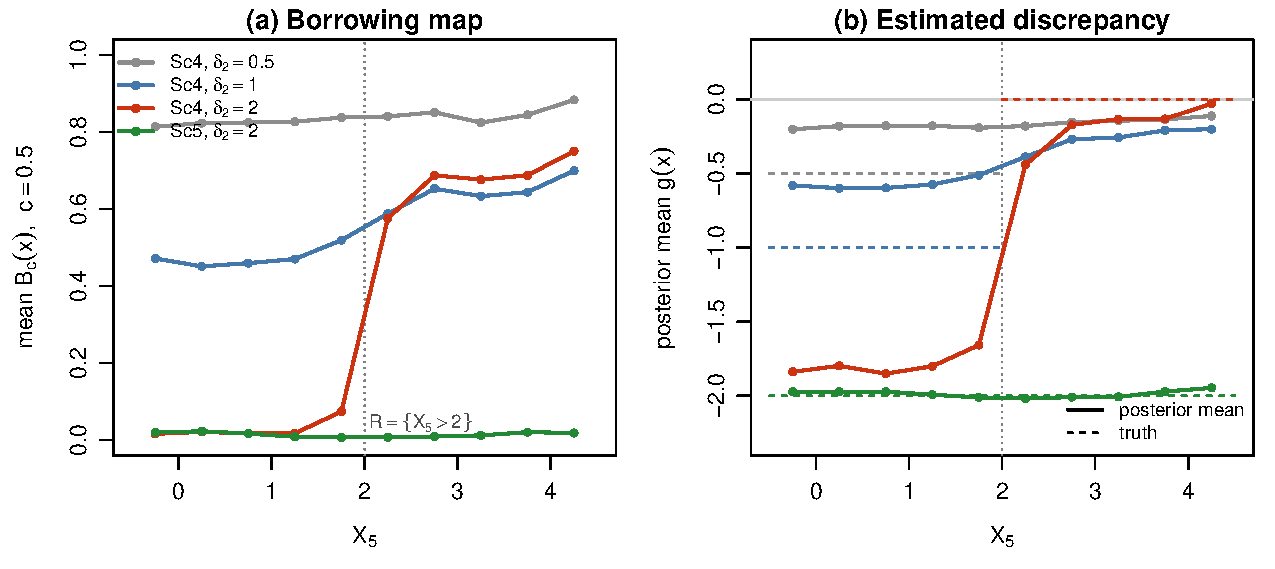
\includegraphics[width=\textwidth]{figures/fig_sc4_map.pdf}
\caption{Regional and global shifts, Gaussian outcomes, LRC-BART ($100$): (a) the borrowing map $\mathcal B_c(x)=P(|g(x)|<0.5\given\text{data})$ and (b) the posterior mean of $g(x)$, both averaged over the RCT control profiles in bins of width $0.5$ on $X_5$ across the first $40$ replicates. The RWD surface is raised by $\delta_2$ where $X_5\le2$ (Sc4) or everywhere (Sc5), so the true discrepancy, dashed in (b), is $-\delta_2$ there.}
\label{fig:sc4map}
\end{figure}

\clearpage
{\color{red}
\begin{table}[htbp]
\centering\color{red}
\caption*{Before revision: Gaussian outcomes, two-arm design, $R=500$ replicates: average treatment effect (ATE) bias, mean posterior SD, Monte Carlo RMSE, coverage of the 95\% credible interval, and power (95\% interval excludes zero at $\delta=1$), with bias and RMSE of the RCT-standardized control mean. Sc4 raises the RWD control surface by $\delta_2$ outside $\mathcal R=\{X_5>2\}$; Sc5 raises it everywhere. LRC-BART (100) targets a prior ESS of 100 RCT controls and LRC-BART (0.9) targets 0.9 of the ESS ceiling; C-BART is LRC-BART with $w=1$. PSCL reports no arm-specific means. The full table with every scenario and method is Web Table~S1.}

\scriptsize
\setlength{\tabcolsep}{3pt}
\renewcommand{\arraystretch}{0.8}
\begin{adjustbox}{max width=\textwidth,max totalheight=0.76\textheight,keepaspectratio}
\begin{tabular}{llccccccc}
\toprule
& & \multicolumn{5}{c}{ATE} & \multicolumn{2}{c}{Control mean} \\
\cmidrule(lr){3-7}\cmidrule(lr){8-9}
Scenario & Method & Bias & SD & RMSE & Cov & Pow & Bias & RMSE \\
\midrule
\multirow{10}{*}{Sc1} & LM-PP & $-$0.002 & 0.347 & 0.337 & 0.94 & 0.85 & 0.001 & 0.243 \\
& BART-NP & 0.004 & 0.203 & 0.220 & 0.91 & 1.00 & 0.001 & 0.185 \\
& BART-CP & 0.008 & 0.145 & 0.142 & 0.96 & 1.00 & $-$0.003 & 0.096 \\
& BART-PP & 0.006 & 0.207 & 0.205 & 0.94 & 1.00 & $-$0.001 & 0.170 \\
& PSCL & 0.005 & 0.269 & 0.261 & 0.95 & 0.97 & $-$0.005 & 0.171 \\
& MAP (100) & 0.006 & 0.292 & 0.265 & 0.97 & 0.95 & $-$0.005 & 0.174 \\
& HierLM & $-$0.003 & 0.338 & 0.341 & 0.93 & 0.85 & 0.003 & 0.249 \\
& C-BART & 0.007 & 0.155 & 0.150 & 0.95 & 1.00 & $-$0.002 & 0.106 \\
& LRC-BART (100) & 0.009 & 0.171 & 0.172 & 0.94 & 1.00 & $-$0.004 & 0.134 \\
& LRC-BART (0.9) & 0.011 & 0.171 & 0.171 & 0.95 & 1.00 & $-$0.005 & 0.132 \\
\midrule
\multirow{10}{*}{Sc2} & LM-PP & 0.010 & 0.340 & 0.331 & 0.95 & 0.84 & $-$0.010 & 0.248 \\
& BART-NP & $-$0.008 & 0.201 & 0.219 & 0.93 & 1.00 & 0.009 & 0.180 \\
& BART-CP & 0.058 & 0.177 & 0.195 & 0.91 & 1.00 & $-$0.056 & 0.151 \\
& BART-PP & 0.007 & 0.208 & 0.204 & 0.96 & 1.00 & $-$0.005 & 0.163 \\
& PSCL & 0.024 & 0.321 & 0.292 & 0.97 & 0.91 & $-$0.029 & 0.205 \\
& MAP (100) & 0.332 & 0.360 & 0.491 & 0.83 & 0.97 & $-$0.337 & 0.424 \\
& HierLM & $-$0.011 & 0.318 & 0.321 & 0.95 & 0.88 & 0.011 & 0.238 \\
& C-BART & 0.042 & 0.168 & 0.186 & 0.91 & 1.00 & $-$0.041 & 0.141 \\
& LRC-BART (100) & 0.023 & 0.181 & 0.192 & 0.94 & 1.00 & $-$0.021 & 0.148 \\
& LRC-BART (0.9) & 0.019 & 0.183 & 0.193 & 0.93 & 1.00 & $-$0.017 & 0.151 \\
\midrule
\multirow{10}{*}{Sc3, $\rho=0$} & LM-PP & 0.043 & 0.356 & 0.346 & 0.95 & 0.85 & $-$0.027 & 0.241 \\
& BART-NP & $-$0.002 & 0.292 & 0.289 & 0.94 & 0.92 & 0.024 & 0.219 \\
& BART-CP & 0.984 & 0.202 & 1.003 & 0.00 & 1.00 & $-$0.962 & 0.971 \\
& BART-PP & 0.029 & 0.275 & 0.273 & 0.94 & 0.96 & $-$0.007 & 0.197 \\
& PSCL & 0.704 & 0.269 & 0.753 & 0.26 & 1.00 & $-$0.693 & 0.713 \\
& MAP (100) & 0.363 & 0.360 & 0.504 & 0.82 & 0.97 & $-$0.352 & 0.431 \\
& HierLM & 0.039 & 0.362 & 0.354 & 0.96 & 0.82 & $-$0.023 & 0.253 \\
& C-BART & 0.226 & 0.300 & 0.380 & 0.87 & 0.98 & $-$0.204 & 0.311 \\
& LRC-BART (100) & 0.041 & 0.284 & 0.280 & 0.94 & 0.96 & $-$0.018 & 0.206 \\
& LRC-BART (0.9) & 0.037 & 0.282 & 0.277 & 0.94 & 0.96 & $-$0.015 & 0.203 \\
\midrule
\multirow{10}{*}{Sc4, $X_5$, $\delta_2=1$} & LM-PP & $-$0.012 & 0.349 & 0.339 & 0.95 & 0.83 & 0.011 & 0.245 \\
& BART-NP & 0.004 & 0.203 & 0.220 & 0.91 & 1.00 & 0.001 & 0.185 \\
& BART-CP & $-$0.338 & 0.146 & 0.368 & 0.35 & 1.00 & 0.343 & 0.357 \\
& BART-PP & $-$0.002 & 0.209 & 0.207 & 0.95 & 1.00 & 0.007 & 0.173 \\
& PSCL & $-$0.246 & 0.271 & 0.358 & 0.87 & 0.80 & 0.247 & 0.300 \\
& MAP (100) & $-$0.224 & 0.306 & 0.361 & 0.91 & 0.75 & 0.224 & 0.292 \\
& HierLM & $-$0.025 & 0.338 & 0.343 & 0.94 & 0.83 & 0.024 & 0.250 \\
& C-BART & $-$0.207 & 0.173 & 0.273 & 0.73 & 1.00 & 0.212 & 0.258 \\
& LRC-BART (100) & $-$0.041 & 0.195 & 0.223 & 0.89 & 1.00 & 0.046 & 0.194 \\
& LRC-BART (0.9) & $-$0.041 & 0.196 & 0.224 & 0.90 & 1.00 & 0.047 & 0.194 \\
\midrule
\multirow{10}{*}{Sc4, $X_5$, $\delta_2=2$} & LM-PP & $-$0.023 & 0.354 & 0.343 & 0.95 & 0.81 & 0.022 & 0.249 \\
& BART-NP & 0.004 & 0.203 & 0.220 & 0.91 & 1.00 & 0.001 & 0.185 \\
& BART-CP & $-$0.685 & 0.149 & 0.701 & 0.00 & 0.56 & 0.690 & 0.698 \\
& BART-PP & $-$0.006 & 0.209 & 0.205 & 0.96 & 1.00 & 0.011 & 0.170 \\
& PSCL & $-$0.498 & 0.273 & 0.562 & 0.54 & 0.44 & 0.498 & 0.528 \\
& MAP (100) & $-$0.377 & 0.333 & 0.495 & 0.78 & 0.46 & 0.378 & 0.437 \\
& HierLM & $-$0.044 & 0.339 & 0.345 & 0.94 & 0.81 & 0.043 & 0.253 \\
& C-BART & $-$0.227 & 0.197 & 0.391 & 0.66 & 0.90 & 0.232 & 0.383 \\
& LRC-BART (100) & 0.000 & 0.189 & 0.202 & 0.92 & 1.00 & 0.005 & 0.168 \\
& LRC-BART (0.9) & $-$0.000 & 0.189 & 0.202 & 0.93 & 1.00 & 0.006 & 0.170 \\
\midrule
\multirow{10}{*}{Sc5, $\delta_2=2$} & LM-PP & $-$0.042 & 0.347 & 0.339 & 0.94 & 0.80 & 0.042 & 0.246 \\
& BART-NP & 0.004 & 0.203 & 0.220 & 0.91 & 1.00 & 0.001 & 0.185 \\
& BART-CP & $-$1.390 & 0.152 & 1.398 & 0.00 & 0.72 & 1.395 & 1.399 \\
& BART-PP & $-$0.012 & 0.208 & 0.205 & 0.95 & 1.00 & 0.017 & 0.171 \\
& PSCL & $-$1.002 & 0.269 & 1.035 & 0.04 & 0.04 & 1.002 & 1.017 \\
& MAP (100) & $-$0.395 & 0.348 & 0.525 & 0.78 & 0.41 & 0.395 & 0.465 \\
& HierLM & $-$0.038 & 0.338 & 0.344 & 0.94 & 0.82 & 0.037 & 0.251 \\
& C-BART & $-$0.316 & 0.194 & 0.650 & 0.76 & 0.93 & 0.322 & 0.648 \\
& LRC-BART (100) & $-$0.001 & 0.190 & 0.203 & 0.92 & 1.00 & 0.005 & 0.171 \\
& LRC-BART (0.9) & $-$0.001 & 0.190 & 0.205 & 0.92 & 1.00 & 0.006 & 0.171 \\
\bottomrule
\end{tabular}
\end{adjustbox}
\end{table}

\clearpage}
{\color{blue}
\begingroup
\singlespacing
\scriptsize
\setlength{\tabcolsep}{2.5pt}
\renewcommand{\arraystretch}{1.0}
\begin{longtable}{llccccccc}
\caption{Gaussian outcomes, two-arm design, $R=500$ replicates: average treatment effect (ATE) bias, mean posterior SD, Monte Carlo RMSE, coverage of the 95\% credible interval, and power (95\% interval excludes zero at $\delta=1$), with bias and RMSE of the RCT-standardized control mean. Sc4 raises the RWD control surface by $\delta_2$ outside $\mathcal R=\{X_5>2\}$; Sc5 raises it everywhere. LRC-BART (100) targets a prior ESS of 100 RCT controls and LRC-BART (0.9) targets 0.9 of the ESS ceiling; CAHB uses $R=200$ paired replicates and our transfer described in Web Appendix~G.2; other rows use $R=500$. C-BART is LRC-BART with $w=1$. PSCL reports no arm-specific means. The full table with every scenario and method is Web Table~S1.}\label{tab:gauss}\\
\toprule
& & \multicolumn{5}{c}{ATE} & \multicolumn{2}{c}{Control mean} \\
\cmidrule(lr){3-7}\cmidrule(lr){8-9}
Scenario & Method & Bias & SD & RMSE & Cov & Pow & Bias & RMSE \\
\midrule
\endfirsthead
\multicolumn{9}{l}{\textit{Table \ref{tab:gauss}, continued}}\\
\toprule
& & \multicolumn{5}{c}{ATE} & \multicolumn{2}{c}{Control mean} \\
\cmidrule(lr){3-7}\cmidrule(lr){8-9}
Scenario & Method & Bias & SD & RMSE & Cov & Pow & Bias & RMSE \\
\midrule
\endhead
\midrule
\endfoot
\bottomrule
\endlastfoot
\multirow{11}{*}{Sc1} & LM-PP & $-$0.002 & 0.347 & 0.337 & 0.94 & 0.85 & 0.001 & 0.243 \\*
& BART-NP & 0.004 & 0.203 & 0.220 & 0.91 & 1.00 & 0.001 & 0.185 \\*
& BART-CP & 0.008 & 0.145 & 0.142 & 0.96 & 1.00 & $-$0.003 & 0.096 \\*
& BART-PP & 0.006 & 0.207 & 0.205 & 0.94 & 1.00 & $-$0.001 & 0.170 \\*
& PSCL & 0.005 & 0.269 & 0.261 & 0.95 & 0.97 & $-$0.005 & 0.171 \\*
& MAP (100) & 0.006 & 0.292 & 0.265 & 0.97 & 0.95 & $-$0.005 & 0.174 \\*
& HierLM & $-$0.003 & 0.338 & 0.341 & 0.93 & 0.85 & 0.003 & 0.249 \\*
& C-BART & 0.007 & 0.155 & 0.150 & 0.95 & 1.00 & $-$0.002 & 0.106 \\*
& LRC-BART (100) & 0.009 & 0.171 & 0.172 & 0.94 & 1.00 & $-$0.004 & 0.134 \\*
& LRC-BART (0.9) & 0.011 & 0.171 & 0.171 & 0.95 & 1.00 & $-$0.005 & 0.132 \\*
& CAHB & $-$0.003 & 0.410 & 0.258 & 1.00 & 0.78 & $-$0.023 & 0.184 \\
\midrule
\multirow{10}{*}{Sc2} & LM-PP & 0.010 & 0.340 & 0.331 & 0.95 & 0.84 & $-$0.010 & 0.248 \\*
& BART-NP & $-$0.008 & 0.201 & 0.219 & 0.93 & 1.00 & 0.009 & 0.180 \\*
& BART-CP & 0.058 & 0.177 & 0.195 & 0.91 & 1.00 & $-$0.056 & 0.151 \\*
& BART-PP & 0.007 & 0.208 & 0.204 & 0.96 & 1.00 & $-$0.005 & 0.163 \\*
& PSCL & 0.024 & 0.321 & 0.292 & 0.97 & 0.91 & $-$0.029 & 0.205 \\*
& MAP (100) & 0.332 & 0.360 & 0.491 & 0.83 & 0.97 & $-$0.337 & 0.424 \\*
& HierLM & $-$0.011 & 0.318 & 0.321 & 0.95 & 0.88 & 0.011 & 0.238 \\*
& C-BART & 0.042 & 0.168 & 0.186 & 0.91 & 1.00 & $-$0.041 & 0.141 \\*
& LRC-BART (100) & 0.023 & 0.181 & 0.192 & 0.94 & 1.00 & $-$0.021 & 0.148 \\*
& LRC-BART (0.9) & 0.019 & 0.183 & 0.193 & 0.93 & 1.00 & $-$0.017 & 0.151 \\
\midrule
\multirow{10}{*}{Sc3, $\rho=0$} & LM-PP & 0.043 & 0.356 & 0.346 & 0.95 & 0.85 & $-$0.027 & 0.241 \\*
& BART-NP & $-$0.002 & 0.292 & 0.289 & 0.94 & 0.92 & 0.024 & 0.219 \\*
& BART-CP & 0.984 & 0.202 & 1.003 & 0.00 & 1.00 & $-$0.962 & 0.971 \\*
& BART-PP & 0.029 & 0.275 & 0.273 & 0.94 & 0.96 & $-$0.007 & 0.197 \\*
& PSCL & 0.704 & 0.269 & 0.753 & 0.26 & 1.00 & $-$0.693 & 0.713 \\*
& MAP (100) & 0.363 & 0.360 & 0.504 & 0.82 & 0.97 & $-$0.352 & 0.431 \\*
& HierLM & 0.039 & 0.362 & 0.354 & 0.96 & 0.82 & $-$0.023 & 0.253 \\*
& C-BART & 0.226 & 0.300 & 0.380 & 0.87 & 0.98 & $-$0.204 & 0.311 \\*
& LRC-BART (100) & 0.041 & 0.284 & 0.280 & 0.94 & 0.96 & $-$0.018 & 0.206 \\*
& LRC-BART (0.9) & 0.037 & 0.282 & 0.277 & 0.94 & 0.96 & $-$0.015 & 0.203 \\
\midrule
\multirow{11}{*}{Sc4, $X_5$, $\delta_2=1$} & LM-PP & $-$0.012 & 0.349 & 0.339 & 0.95 & 0.83 & 0.011 & 0.245 \\*
& BART-NP & 0.004 & 0.203 & 0.220 & 0.91 & 1.00 & 0.001 & 0.185 \\*
& BART-CP & $-$0.338 & 0.146 & 0.368 & 0.35 & 1.00 & 0.343 & 0.357 \\*
& BART-PP & $-$0.002 & 0.209 & 0.207 & 0.95 & 1.00 & 0.007 & 0.173 \\*
& PSCL & $-$0.246 & 0.271 & 0.358 & 0.87 & 0.80 & 0.247 & 0.300 \\*
& MAP (100) & $-$0.224 & 0.306 & 0.361 & 0.91 & 0.75 & 0.224 & 0.292 \\*
& HierLM & $-$0.025 & 0.338 & 0.343 & 0.94 & 0.83 & 0.024 & 0.250 \\*
& C-BART & $-$0.207 & 0.173 & 0.273 & 0.73 & 1.00 & 0.212 & 0.258 \\*
& LRC-BART (100) & $-$0.041 & 0.195 & 0.223 & 0.89 & 1.00 & 0.046 & 0.194 \\*
& LRC-BART (0.9) & $-$0.041 & 0.196 & 0.224 & 0.90 & 1.00 & 0.047 & 0.194 \\*
& CAHB & $-$0.208 & 0.413 & 0.333 & 0.98 & 0.42 & 0.181 & 0.262 \\
\midrule
\multirow{11}{*}{Sc4, $X_5$, $\delta_2=2$} & LM-PP & $-$0.023 & 0.354 & 0.343 & 0.95 & 0.81 & 0.022 & 0.249 \\*
& BART-NP & 0.004 & 0.203 & 0.220 & 0.91 & 1.00 & 0.001 & 0.185 \\*
& BART-CP & $-$0.685 & 0.149 & 0.701 & 0.00 & 0.56 & 0.690 & 0.698 \\*
& BART-PP & $-$0.006 & 0.209 & 0.205 & 0.96 & 1.00 & 0.011 & 0.170 \\*
& PSCL & $-$0.498 & 0.273 & 0.562 & 0.54 & 0.44 & 0.498 & 0.528 \\*
& MAP (100) & $-$0.377 & 0.333 & 0.495 & 0.78 & 0.46 & 0.378 & 0.437 \\*
& HierLM & $-$0.044 & 0.339 & 0.345 & 0.94 & 0.81 & 0.043 & 0.253 \\*
& C-BART & $-$0.227 & 0.197 & 0.391 & 0.66 & 0.90 & 0.232 & 0.383 \\*
& LRC-BART (100) & 0.000 & 0.189 & 0.202 & 0.92 & 1.00 & 0.005 & 0.168 \\*
& LRC-BART (0.9) & $-$0.000 & 0.189 & 0.202 & 0.93 & 1.00 & 0.006 & 0.170 \\*
& CAHB & $-$0.333 & 0.422 & 0.453 & 0.95 & 0.25 & 0.309 & 0.398 \\
\midrule
\multirow{11}{*}{Sc5, $\delta_2=2$} & LM-PP & $-$0.042 & 0.347 & 0.339 & 0.94 & 0.80 & 0.042 & 0.246 \\*
& BART-NP & 0.004 & 0.203 & 0.220 & 0.91 & 1.00 & 0.001 & 0.185 \\*
& BART-CP & $-$1.390 & 0.152 & 1.398 & 0.00 & 0.72 & 1.395 & 1.399 \\*
& BART-PP & $-$0.012 & 0.208 & 0.205 & 0.95 & 1.00 & 0.017 & 0.171 \\*
& PSCL & $-$1.002 & 0.269 & 1.035 & 0.04 & 0.04 & 1.002 & 1.017 \\*
& MAP (100) & $-$0.395 & 0.348 & 0.525 & 0.78 & 0.41 & 0.395 & 0.465 \\*
& HierLM & $-$0.038 & 0.338 & 0.344 & 0.94 & 0.82 & 0.037 & 0.251 \\*
& C-BART & $-$0.316 & 0.194 & 0.650 & 0.76 & 0.93 & 0.322 & 0.648 \\*
& LRC-BART (100) & $-$0.001 & 0.190 & 0.203 & 0.92 & 1.00 & 0.005 & 0.171 \\*
& LRC-BART (0.9) & $-$0.001 & 0.190 & 0.205 & 0.92 & 1.00 & 0.006 & 0.171 \\*
& CAHB & $-$0.067 & 0.479 & 0.400 & 0.95 & 0.52 & 0.041 & 0.326 \\
\end{longtable}
\endgroup

\clearpage}

\clearpage
{\color{red}
\begin{table}[htbp]
\centering\color{red}
\caption*{Before revision: Regional and global shifts, Gaussian outcomes, $R=500$: ATE bias and coverage; RMSE of the posterior mean control surface over the RCT profiles inside the compatible region $\mathcal R$ and outside it; the borrowing map $\mathcal B_c(x)=P(|g(x)|<0.5\mid\text{data})$ averaged over the RCT control profiles in each region; the posterior mean of $g(x)$ averaged over each region (true value $0$ in $\mathcal R$ and $-\delta_2$ in $\mathcal R^c$); and the realized ESS. In Sc5 the compatible region is empty. Sc4$'$ places the shift on the null covariate $X_7$. LRC-BART ($w=0$) has no spike, so its map reflects the slab alone.}

\scriptsize
\setlength{\tabcolsep}{3pt}
\renewcommand{\arraystretch}{0.8}
\resizebox{\textwidth}{!}{%
\begin{adjustbox}{max width=\textwidth,max totalheight=0.76\textheight,keepaspectratio}
\begin{tabular}{llccccccccc}
\toprule
& & \multicolumn{2}{c}{ATE} & \multicolumn{2}{c}{Surface RMSE} & \multicolumn{2}{c}{$\bar{\mathcal B}_c$} & \multicolumn{2}{c}{Mean $\hat g$} & \\
\cmidrule(lr){3-4}\cmidrule(lr){5-6}\cmidrule(lr){7-8}\cmidrule(lr){9-10}
Scenario & Method & Bias & Cov & $\mathcal R$ & $\mathcal R^c$ & $\mathcal R$ & $\mathcal R^c$ & $\mathcal R$ & $\mathcal R^c$ & ESS \\
\midrule
\multirow{4}{*}{Sc4 (0.5)} & BART-PP & 0.000 & 0.95 & 0.758 & 0.795 & --- & --- & --- & --- & --- \\
& C-BART & $-$0.109 & 0.90 & 0.736 & 0.799 & 0.98 & 0.98 & $-$0.06 & $-$0.06 & 79.4 \\
& LRC-BART ($w=0$) & 0.007 & 0.93 & 0.768 & 0.795 & 0.71 & 0.69 & $-$0.21 & $-$0.27 & 0.1 \\
& LRC-BART (100) & $-$0.043 & 0.92 & 0.751 & 0.796 & 0.84 & 0.83 & $-$0.15 & $-$0.18 & 42.9 \\
\midrule
\multirow{4}{*}{Sc4 (1)} & BART-PP & $-$0.002 & 0.95 & 0.784 & 0.820 & --- & --- & --- & --- & --- \\
& C-BART & $-$0.207 & 0.73 & 0.749 & 0.915 & 0.91 & 0.90 & $-$0.14 & $-$0.16 & 73.6 \\
& LRC-BART ($w=0$) & 0.006 & 0.93 & 0.801 & 0.827 & 0.51 & 0.40 & $-$0.35 & $-$0.63 & 0.1 \\
& LRC-BART (100) & $-$0.041 & 0.89 & 0.783 & 0.843 & 0.62 & 0.52 & $-$0.32 & $-$0.52 & 20.8 \\
\midrule
\multirow{4}{*}{Sc4 (2)} & BART-PP & $-$0.006 & 0.96 & 0.785 & 0.822 & --- & --- & --- & --- & --- \\
& C-BART & $-$0.227 & 0.66 & 0.801 & 1.087 & 0.66 & 0.39 & $-$0.30 & $-$0.97 & 45.7 \\
& LRC-BART ($w=0$) & 0.004 & 0.92 & 0.836 & 0.858 & 0.57 & 0.05 & $-$0.25 & $-$1.73 & 0.1 \\
& LRC-BART (100) & 0.000 & 0.92 & 0.824 & 0.857 & 0.64 & 0.05 & $-$0.26 & $-$1.71 & 0.8 \\
\midrule
\multirow{4}{*}{Sc4$'$ (1)} & BART-PP & $-$0.001 & 0.96 & 0.807 & 0.810 & --- & --- & --- & --- & --- \\
& C-BART & $-$0.206 & 0.73 & 0.767 & 0.899 & 0.91 & 0.90 & $-$0.15 & $-$0.16 & 73.3 \\
& LRC-BART ($w=0$) & 0.009 & 0.92 & 0.820 & 0.817 & 0.52 & 0.41 & $-$0.37 & $-$0.63 & 0.1 \\
& LRC-BART (100) & $-$0.038 & 0.90 & 0.805 & 0.833 & 0.62 & 0.52 & $-$0.33 & $-$0.52 & 20.5 \\
\midrule
\multirow{4}{*}{Sc4$'$ (2)} & BART-PP & $-$0.002 & 0.95 & 0.805 & 0.806 & --- & --- & --- & --- & --- \\
& C-BART & $-$0.218 & 0.69 & 0.828 & 1.075 & 0.64 & 0.38 & $-$0.33 & $-$0.97 & 44.7 \\
& LRC-BART ($w=0$) & 0.007 & 0.92 & 0.859 & 0.848 & 0.57 & 0.05 & $-$0.25 & $-$1.74 & 0.1 \\
& LRC-BART (100) & 0.001 & 0.93 & 0.850 & 0.848 & 0.64 & 0.05 & $-$0.26 & $-$1.71 & 0.8 \\
\midrule
\multirow{4}{*}{Sc5 (1)} & BART-PP & $-$0.004 & 0.95 & --- & 0.769 & --- & --- & --- & --- & --- \\
& C-BART & $-$0.244 & 0.68 & --- & 0.821 & --- & 0.43 & --- & $-$0.60 & 41.5 \\
& LRC-BART ($w=0$) & 0.007 & 0.92 & --- & 0.769 & --- & 0.10 & --- & $-$1.00 & 0.1 \\
& LRC-BART (100) & $-$0.005 & 0.91 & --- & 0.768 & --- & 0.10 & --- & $-$0.98 & 1.2 \\
\midrule
\multirow{4}{*}{Sc5 (2)} & BART-PP & $-$0.012 & 0.95 & --- & 0.771 & --- & --- & --- & --- & --- \\
& C-BART & $-$0.316 & 0.76 & --- & 0.932 & --- & 0.19 & --- & $-$1.54 & 45.4 \\
& LRC-BART ($w=0$) & 0.006 & 0.93 & --- & 0.771 & --- & 0.01 & --- & $-$2.00 & 0.1 \\
& LRC-BART (100) & $-$0.001 & 0.92 & --- & 0.771 & --- & 0.01 & --- & $-$1.99 & 0.2 \\
\bottomrule
\end{tabular}
\end{adjustbox}
}
\end{table}

\clearpage}
{\color{blue}
\begingroup
\singlespacing
\scriptsize
\setlength{\tabcolsep}{2.5pt}
\renewcommand{\arraystretch}{1.0}
\begin{longtable}{llccccccccc}
\caption{Regional and global shifts, Gaussian outcomes, $R=500$: ATE bias and coverage; RMSE of the posterior mean control surface over all $N$ RCT profiles (treated and control) inside the compatible region $\mathcal R$ and outside it; the borrowing map $\mathcal B_c(x)=P(|g(x)|<0.5\mid\text{data})$ averaged over the RCT control profiles in each region; the posterior mean of $g(x)$ averaged over each region (true value $0$ in $\mathcal R$ and $-\delta_2$ in $\mathcal R^c$); and the realized ESS. In Sc5 the compatible region is empty. Sc4$'$ places the shift on the null covariate $X_7$. LRC-BART ($w=0$) has no spike, so its map reflects the slab alone. CAHB rows use $R=200$; all other rows use $R=500$. CAHB precision shares and effective sizes have different definitions and are reported separately in Web Appendix~G.2. For Sc1, the two columns use the Sc4 partition although both regions are compatible.}\label{tab:map}\\
\toprule
& & \multicolumn{2}{c}{ATE} & \multicolumn{2}{c}{Surface RMSE} & \multicolumn{2}{c}{$\bar{\mathcal B}_c$} & \multicolumn{2}{c}{Mean $\hat g$} & \\
\cmidrule(lr){3-4}\cmidrule(lr){5-6}\cmidrule(lr){7-8}\cmidrule(lr){9-10}
Scenario & Method & Bias & Cov & $\mathcal R$ & $\mathcal R^c$ & $\mathcal R$ & $\mathcal R^c$ & $\mathcal R$ & $\mathcal R^c$ & ESS \\
\midrule
\endfirsthead
\multicolumn{11}{l}{\textit{Table \ref{tab:map}, continued}}\\
\toprule
& & \multicolumn{2}{c}{ATE} & \multicolumn{2}{c}{Surface RMSE} & \multicolumn{2}{c}{$\bar{\mathcal B}_c$} & \multicolumn{2}{c}{Mean $\hat g$} & \\
\cmidrule(lr){3-4}\cmidrule(lr){5-6}\cmidrule(lr){7-8}\cmidrule(lr){9-10}
Scenario & Method & Bias & Cov & $\mathcal R$ & $\mathcal R^c$ & $\mathcal R$ & $\mathcal R^c$ & $\mathcal R$ & $\mathcal R^c$ & ESS \\
\midrule
\endhead
\midrule
\endfoot
\bottomrule
\endlastfoot
\multirow{5}{*}{Sc1} & BART-PP & 0.006 & 0.94 & 0.750 & 0.780 & --- & --- & --- & --- & --- \\*
& C-BART & 0.007 & 0.95 & 0.728 & 0.756 & 1.00 & 1.00 & 0.00 & 0.00 & 81.0 \\*
& LRC-BART ($w=0$) & 0.009 & 0.92 & 0.755 & 0.783 & 0.79 & 0.79 & $-$0.00 & 0.01 & 0.1 \\*
& LRC-BART (100) & 0.009 & 0.94 & 0.736 & 0.763 & 0.92 & 0.92 & $-$0.00 & 0.00 & 52.5 \\*
& CAHB & $-$0.003 & 1.00 & 2.071 & 2.273 & --- & --- & --- & --- & --- \\
\midrule
\multirow{4}{*}{Sc4 (0.5)} & BART-PP & 0.000 & 0.95 & 0.758 & 0.795 & --- & --- & --- & --- & --- \\*
& C-BART & $-$0.109 & 0.90 & 0.736 & 0.799 & 0.98 & 0.98 & $-$0.06 & $-$0.06 & 79.4 \\*
& LRC-BART ($w=0$) & 0.007 & 0.93 & 0.768 & 0.795 & 0.71 & 0.69 & $-$0.21 & $-$0.27 & 0.1 \\*
& LRC-BART (100) & $-$0.043 & 0.92 & 0.751 & 0.796 & 0.84 & 0.83 & $-$0.15 & $-$0.18 & 42.9 \\
\midrule
\multirow{5}{*}{Sc4 (1)} & BART-PP & $-$0.002 & 0.95 & 0.784 & 0.820 & --- & --- & --- & --- & --- \\*
& C-BART & $-$0.207 & 0.73 & 0.749 & 0.915 & 0.91 & 0.90 & $-$0.14 & $-$0.16 & 73.6 \\*
& LRC-BART ($w=0$) & 0.006 & 0.93 & 0.801 & 0.827 & 0.51 & 0.40 & $-$0.35 & $-$0.63 & 0.1 \\*
& LRC-BART (100) & $-$0.041 & 0.89 & 0.783 & 0.843 & 0.62 & 0.52 & $-$0.32 & $-$0.52 & 20.8 \\*
& CAHB & $-$0.208 & 0.98 & 2.133 & 2.207 & --- & --- & --- & --- & --- \\
\midrule
\multirow{5}{*}{Sc4 (2)} & BART-PP & $-$0.006 & 0.96 & 0.785 & 0.822 & --- & --- & --- & --- & --- \\*
& C-BART & $-$0.227 & 0.66 & 0.801 & 1.087 & 0.66 & 0.39 & $-$0.30 & $-$0.97 & 45.7 \\*
& LRC-BART ($w=0$) & 0.004 & 0.92 & 0.836 & 0.858 & 0.57 & 0.05 & $-$0.25 & $-$1.73 & 0.1 \\*
& LRC-BART (100) & 0.000 & 0.92 & 0.824 & 0.857 & 0.64 & 0.05 & $-$0.26 & $-$1.71 & 0.8 \\*
& CAHB & $-$0.333 & 0.95 & 2.172 & 2.157 & --- & --- & --- & --- & --- \\
\midrule
\multirow{4}{*}{Sc4$'$ (1)} & BART-PP & $-$0.001 & 0.96 & 0.807 & 0.810 & --- & --- & --- & --- & --- \\*
& C-BART & $-$0.206 & 0.73 & 0.767 & 0.899 & 0.91 & 0.90 & $-$0.15 & $-$0.16 & 73.3 \\*
& LRC-BART ($w=0$) & 0.009 & 0.92 & 0.820 & 0.817 & 0.52 & 0.41 & $-$0.37 & $-$0.63 & 0.1 \\*
& LRC-BART (100) & $-$0.038 & 0.90 & 0.805 & 0.833 & 0.62 & 0.52 & $-$0.33 & $-$0.52 & 20.5 \\
\midrule
\multirow{4}{*}{Sc4$'$ (2)} & BART-PP & $-$0.002 & 0.95 & 0.805 & 0.806 & --- & --- & --- & --- & --- \\*
& C-BART & $-$0.218 & 0.69 & 0.828 & 1.075 & 0.64 & 0.38 & $-$0.33 & $-$0.97 & 44.7 \\*
& LRC-BART ($w=0$) & 0.007 & 0.92 & 0.859 & 0.848 & 0.57 & 0.05 & $-$0.25 & $-$1.74 & 0.1 \\*
& LRC-BART (100) & 0.001 & 0.93 & 0.850 & 0.848 & 0.64 & 0.05 & $-$0.26 & $-$1.71 & 0.8 \\
\midrule
\multirow{5}{*}{Sc5 (1)} & BART-PP & $-$0.004 & 0.95 & --- & 0.769 & --- & --- & --- & --- & --- \\*
& C-BART & $-$0.244 & 0.68 & --- & 0.821 & --- & 0.43 & --- & $-$0.60 & 41.5 \\*
& LRC-BART ($w=0$) & 0.007 & 0.92 & --- & 0.769 & --- & 0.10 & --- & $-$1.00 & 0.1 \\*
& LRC-BART (100) & $-$0.005 & 0.91 & --- & 0.768 & --- & 0.10 & --- & $-$0.98 & 1.2 \\*
& CAHB & $-$0.437 & 0.91 & --- & 2.203 & --- & --- & --- & --- & --- \\
\midrule
\multirow{5}{*}{Sc5 (2)} & BART-PP & $-$0.012 & 0.95 & --- & 0.771 & --- & --- & --- & --- & --- \\*
& C-BART & $-$0.316 & 0.76 & --- & 0.932 & --- & 0.19 & --- & $-$1.54 & 45.4 \\*
& LRC-BART ($w=0$) & 0.006 & 0.93 & --- & 0.771 & --- & 0.01 & --- & $-$2.00 & 0.1 \\*
& LRC-BART (100) & $-$0.001 & 0.92 & --- & 0.771 & --- & 0.01 & --- & $-$1.99 & 0.2 \\*
& CAHB & $-$0.067 & 0.95 & --- & 1.983 & --- & --- & --- & --- & --- \\
\end{longtable}
\endgroup
\begin{center}\scriptsize
\par\medskip
\begin{tabular}{lcc}
\toprule
Scenario & Regional ESS, $X_5>2$ & Regional ESS, $X_5\le2$ \\
\midrule
Sc1 & 32.66 & 31.86 \\
Sc4 (1) & 15.14 & 12.74 \\
Sc4 (2) & 9.51 & 0.44 \\
Sc5 (2) & 0.24 & 0.24 \\
\bottomrule
\end{tabular}
\par\smallskip\parbox{\textwidth}{\scriptsize Regional realized ESS for LRC-BART (100), averaged over the first 200 paired replicates. Each estimand is the control mean standardized to all RCT profiles in that region. The partition is held fixed for Sc1 and Sc5; both regions are compatible in Sc1 and neither is compatible in Sc5. Regional effective sizes are not additive.}
\end{center}

\clearpage}


\subsection{Survival outcomes}
\label{sec:sim_surv}

Table~\ref{tab:surv} reports the survival study for the median ratio and the RMST ratio side by side, and Web Table~S2 the full set. With $75$ RCT controls and about a quarter of the times censored, the median ratio has a wide and skewed posterior under every method, and its posterior mean carries an upward bias that grows with the posterior spread: BART-NP has bias $0.26$ and RMSE $0.51$ in Sc1, where its RMST-ratio bias is $0.13$, and AFT-NP is wider still. Borrowing \DIFdelbegin \DIFdel{is what makes the estimand usable at this }\DIFdelend \DIFaddbegin \DIFadd{reduces this uncertainty at the studied }\DIFaddend sample size. 
\DIFaddbegin 

\DIFaddend In Sc1 LRC-BART ($100$) has median-ratio bias $0.045$ and RMSE $0.312$ against $0.032$ and $0.345$ for BART-PP, with power $0.34$ against $0.25$, and its RMST-ratio RMSE is $0.097$ against $0.106$; in Sc2, where the ceiling falls to $40$ and the absolute targets are capped, the two are within $0.03$ of each other on both estimands. 
\DIFaddbegin 

\DIFaddend Under unmeasured confounding \DIFdelbegin \DIFdel{, }\DIFdelend \DIFaddbegin \DIFadd{(}\DIFaddend Sc3\DIFaddbegin \DIFadd{)}\DIFaddend , the tree models with a fixed commensurate component \DIFdelbegin \DIFdel{fail }\DIFdelend \DIFaddbegin \DIFadd{have large biases, }\DIFaddend as in the Gaussian study\DIFdelbegin \DIFdel{, }\DIFdelend \DIFaddbegin \DIFadd{: }\DIFaddend BART-CP with median-ratio bias $2.3$ and C-BART with $0.58$ at $\rho=0$, and LRC-BART abstains with a realized ESS of $2.3$. Its median-ratio bias is then $0.15$ against $0.04$ for BART-PP and $0.19$ for BART-NP, with RMSE $0.558$ against $0.451$ and coverage $0.94$; the paired difference in bias from BART-PP is $0.11$ with standard error $0.005$, the largest loss to BART-PP in the study. The control log-median is biased by only $0.02$, against $-0.006$ for BART-PP, so most of the difference on the ratio scale comes from the wider posterior LRC-BART has once it has switched borrowing off with $75$ controls, \DIFdelbegin \DIFdel{a posterior SD of }\DIFdelend \DIFaddbegin \DIFadd{with posterior SD }\DIFaddend $0.52$ against $0.39$, \DIFdelbegin \DIFdel{passed through the convex ratio }\DIFdelend \DIFaddbegin \DIFadd{together with the nonlinear transformation to the ratio scale}\DIFaddend . On the RMST ratio the biases are $0.031$ and $-0.005$ and the RMSEs $0.146$ and $0.137$, a paired difference in mean squared error of $0.003$ with standard error $0.001$. We report both estimands because the median ratio amplifies a small control bias and a wide posterior in a way the RMST ratio does not, and the RMST ratio is the estimand of the application. 
\DIFaddbegin 

\DIFaddend Under the regional shift, Sc4 at $\delta_2=1$ on the log scale with a residual SD of $1.4$, the map separates weakly, $0.64$ in $\mathcal R$ against $0.58$ outside, \DIFdelbegin \DIFdel{yet the ATE stays unbiased (}\DIFdelend \DIFaddbegin \DIFadd{and the treatment-effect biases are }\DIFaddend $-0.011$ on the median ratio \DIFdelbegin \DIFdel{, }\DIFdelend \DIFaddbegin \DIFadd{and }\DIFaddend $-0.037$ on the RMST ratio \DIFdelbegin \DIFdel{) }\DIFdelend where C-BART and BART-CP have biases of $-0.20$ and $-0.37$; under the global shift of Sc5 the map is $0.16$, the median-ratio bias $0.03$, and C-BART's $-0.23$. Web Table~S4 gives the map and surface summaries for the survival study, and the fractional ladder behaves as in the Gaussian study.

\begin{table}[htbp]
\centering
\singlespacing
\caption{Survival outcomes, two-arm design, $R=500$: bias, Monte Carlo RMSE, coverage and power (95\% interval excludes one) for the ratio of standardized population medians (true value $1.4$) and the ratio of standardized restricted mean survival times at $t^\ast=3$. Sc4 raises the RWD log-time surface by $\delta_2=1$ outside $\mathcal R=\{X_5>2\}$ and Sc5 by $1$ everywhere. Point estimates are posterior means. The full table is Web Table~S2.}
\label{tab:surv}
\scriptsize
\setlength{\tabcolsep}{4pt}
\renewcommand{\arraystretch}{0.8}
\begin{adjustbox}{max width=\textwidth,max totalheight=0.68\textheight}
\begin{tabular}{llcccccccc}
\toprule
& & \multicolumn{4}{c}{Median ratio} & \multicolumn{4}{c}{RMST ratio, $t^\ast=3$} \\
\cmidrule(lr){3-6}\cmidrule(lr){7-10}
Scenario & Method & Bias & RMSE & Cov & Pow & Bias & RMSE & Cov & Pow \\
\midrule
\multirow{8}{*}{Sc1} & AFT-PP & 0.261 & 0.737 & 0.95 & 0.12 & $-$0.009 & 0.142 & 0.94 & 0.10 \\
& BART-NP & 0.260 & 0.511 & 0.92 & 0.46 & 0.131 & 0.206 & 0.87 & 0.47 \\
& BART-CP & 0.064 & 0.232 & 0.96 & 0.63 & $-$0.011 & 0.072 & 0.95 & 0.35 \\
& BART-PP & 0.032 & 0.345 & 0.95 & 0.25 & $-$0.023 & 0.106 & 0.94 & 0.17 \\
& HierAFT & 0.246 & 0.733 & 0.94 & 0.12 & $-$0.008 & 0.152 & 0.92 & 0.11 \\
& C-BART & 0.034 & 0.248 & 0.97 & 0.42 & 0.003 & 0.079 & 0.95 & 0.32 \\
& LRC-BART (100) & 0.045 & 0.312 & 0.95 & 0.34 & 0.003 & 0.097 & 0.94 & 0.28 \\
& LRC-BART (0.9) & 0.042 & 0.304 & 0.96 & 0.38 & 0.002 & 0.095 & 0.95 & 0.30 \\
\midrule
\multirow{8}{*}{Sc2} & AFT-PP & 0.389 & 0.818 & 0.95 & 0.19 & 0.050 & 0.154 & 0.95 & 0.20 \\
& BART-NP & 0.251 & 0.495 & 0.91 & 0.43 & 0.110 & 0.177 & 0.88 & 0.45 \\
& BART-CP & 0.194 & 0.383 & 0.93 & 0.56 & 0.037 & 0.100 & 0.94 & 0.43 \\
& BART-PP & 0.036 & 0.335 & 0.95 & 0.24 & $-$0.002 & 0.097 & 0.95 & 0.21 \\
& HierAFT & 0.233 & 0.695 & 0.97 & 0.14 & 0.001 & 0.134 & 0.95 & 0.12 \\
& C-BART & 0.138 & 0.331 & 0.93 & 0.55 & 0.043 & 0.104 & 0.92 & 0.49 \\
& LRC-BART (100) & 0.061 & 0.322 & 0.94 & 0.34 & 0.018 & 0.100 & 0.93 & 0.31 \\
& LRC-BART (0.9) & 0.058 & 0.325 & 0.94 & 0.33 & 0.017 & 0.100 & 0.94 & 0.30 \\
\midrule
\multirow{8}{*}{Sc3, $\rho=0$} & AFT-PP & 0.440 & 0.919 & 0.94 & 0.19 & 0.054 & 0.158 & 0.95 & 0.19 \\
& BART-NP & 0.186 & 0.571 & 0.90 & 0.30 & 0.058 & 0.173 & 0.92 & 0.21 \\
& BART-CP & 2.308 & 2.412 & 0.00 & 1.00 & 0.588 & 0.607 & 0.01 & 1.00 \\
& BART-PP & 0.041 & 0.451 & 0.91 & 0.20 & $-$0.005 & 0.137 & 0.92 & 0.15 \\
& HierAFT & 0.337 & 0.890 & 0.95 & 0.13 & 0.006 & 0.147 & 0.95 & 0.11 \\
& C-BART & 0.576 & 0.909 & 0.88 & 0.40 & 0.139 & 0.222 & 0.85 & 0.38 \\
& LRC-BART (100) & 0.155 & 0.558 & 0.94 & 0.17 & 0.031 & 0.146 & 0.94 & 0.18 \\
& LRC-BART (0.9) & 0.148 & 0.554 & 0.94 & 0.17 & 0.029 & 0.144 & 0.93 & 0.18 \\
\midrule
\multirow{8}{*}{Sc4, $X_5$, $\delta_2=1$} & AFT-PP & 0.191 & 0.691 & 0.95 & 0.10 & $-$0.039 & 0.139 & 0.92 & 0.07 \\
& BART-NP & 0.260 & 0.511 & 0.92 & 0.46 & 0.131 & 0.206 & 0.87 & 0.47 \\
& BART-CP & $-$0.367 & 0.401 & 0.50 & 0.04 & $-$0.156 & 0.168 & 0.32 & 0.07 \\
& BART-PP & $-$0.012 & 0.339 & 0.97 & 0.17 & $-$0.059 & 0.113 & 0.91 & 0.07 \\
& HierAFT & 0.193 & 0.700 & 0.94 & 0.10 & $-$0.023 & 0.149 & 0.91 & 0.09 \\
& C-BART & $-$0.202 & 0.305 & 0.84 & 0.08 & $-$0.093 & 0.120 & 0.79 & 0.04 \\
& LRC-BART (100) & $-$0.011 & 0.340 & 0.93 & 0.24 & $-$0.037 & 0.108 & 0.90 & 0.16 \\
& LRC-BART (0.9) & $-$0.018 & 0.342 & 0.93 & 0.24 & $-$0.040 & 0.110 & 0.90 & 0.16 \\
\midrule
\multirow{8}{*}{Sc5, $\delta_2=1$} & AFT-PP & 0.193 & 0.695 & 0.94 & 0.09 & $-$0.029 & 0.141 & 0.93 & 0.08 \\
& BART-NP & 0.260 & 0.511 & 0.92 & 0.46 & 0.131 & 0.206 & 0.87 & 0.47 \\
& BART-CP & $-$0.703 & 0.712 & 0.00 & 0.64 & $-$0.256 & 0.262 & 0.01 & 0.65 \\
& BART-PP & $-$0.029 & 0.333 & 0.95 & 0.17 & $-$0.041 & 0.110 & 0.93 & 0.11 \\
& HierAFT & 0.204 & 0.701 & 0.94 & 0.10 & $-$0.018 & 0.150 & 0.92 & 0.09 \\
& C-BART & $-$0.233 & 0.405 & 0.77 & 0.13 & $-$0.085 & 0.143 & 0.77 & 0.11 \\
& LRC-BART (100) & 0.032 & 0.353 & 0.93 & 0.30 & 0.001 & 0.112 & 0.93 & 0.26 \\
& LRC-BART (0.9) & 0.029 & 0.350 & 0.94 & 0.31 & 0.001 & 0.111 & 0.94 & 0.26 \\
\bottomrule
\end{tabular}
\end{adjustbox}
\end{table}


\subsection{The single-arm design}
\label{sec:sim_single}

\DIFdelbegin \DIFdel{The application }\DIFdelend \DIFaddbegin \DIFadd{To assess the single-arm setting }\DIFaddend of Section~\ref{sec:application}\DIFdelbegin \DIFdel{has no RCT control arm, and we study that design with the mechanisms above}\DIFdelend \DIFaddbegin \DIFadd{, we use the same mechanisms with no RCT control arm}\DIFaddend : the trial contributes $n_T$ treated subjects only, $200$ for Gaussian outcomes and $30$ or $200$ for survival outcomes, the $300$ RWD controls are the sole control source, and LRC-BART runs in the single-arm mode of Section~\ref{sec:singlearm} with $w=1$ against the complete-pooling models, the hierarchical models and BART-CP; Sc3 is not identifiable without an internal control and is omitted. Table~\ref{tab:single} reports the results and Web Appendix~G.7 discusses them in detail. Under Sc1 the tree models have Gaussian RMSE $0.16$ with coverage $0.94$ to $1.00$. 
\DIFaddbegin 

\DIFaddend Under Sc2\DIFdelbegin \DIFdel{no method does well, }\DIFdelend \DIFaddbegin \DIFadd{, all methods have substantial bias }\DIFaddend because without RCT controls \DIFdelbegin \DIFdel{nothing in the data can reveal a }\DIFdelend \DIFaddbegin \DIFadd{the data cannot identify a control }\DIFaddend discrepancy at trial profiles \DIFdelbegin \DIFdel{the RWD does not cover}\DIFdelend \DIFaddbegin \DIFadd{without RWD support}\DIFaddend : on the Gaussian ATE, BART-CP has bias $0.41$ with coverage $0.75$ and LRC-BART $0.42$. In every design LRC-BART ($100$) gives the point estimate of the pooled model within $0.005$, with a wider posterior where the target is not capped, and the $w=0.9$ sensitivity only adds prior noise to the counterfactual control, which is why we report $w=1$ in single-arm mode.

\begingroup
\singlespacing
\scriptsize
\setlength{\tabcolsep}{2.5pt}
\renewcommand{\arraystretch}{1.0}
\begin{longtable}{llcccccccc}
\caption{Single-arm design, $R=500$: the trial contributes $n_T$ treated subjects only and the $n_2=300$ RWD controls are the sole control source, under Sc1 (no confounding) and Sc2 (measured confounding). LRC-BART (pooled) is $w=1$ with the spike scale at the grid minimum, LRC-BART (0.9) is $w=1$ at 0.9 of the ESS ceiling, and LRC-BART ($w=0.9$) is the slab sensitivity at the absolute target 100. HierLM and HierAFT use the stated hyperprior $\tau_j^2\sim$ Inv-Gamma$(1.5,0.75)$ with no RCT controls, under which the control surface is drawn from the hierarchy; values above $10^3$ are printed as such. Control columns are on the outcome scale (Gaussian) or the log-median scale (survival). Web Table~S6 adds the absolute-target rows and the median ratio at $n_T=200$.}\label{tab:single}\\
\toprule
& & \multicolumn{5}{c}{Treatment effect} & \multicolumn{2}{c}{Control} & \\
\cmidrule(lr){3-7}\cmidrule(lr){8-9}
Design & Method & Bias & SD & RMSE & Cov & Pow & Bias & RMSE & Prior ESS \\
\midrule
\endfirsthead
\multicolumn{10}{l}{\textit{Table \ref{tab:single}, continued}}\\
\toprule
& & \multicolumn{5}{c}{Treatment effect} & \multicolumn{2}{c}{Control} & \\
\cmidrule(lr){3-7}\cmidrule(lr){8-9}
Design & Method & Bias & SD & RMSE & Cov & Pow & Bias & RMSE & Prior ESS \\
\midrule
\endhead
\midrule
\endfoot
\bottomrule
\endlastfoot
\multirow{6}{*}{\shortstack[l]{Gaussian, $n_T=200$\\ATE\\Sc1}} & LM-CP & 0.007 & 0.259 & 0.254 & 0.95 & 0.97 & $-$0.003 & 0.233 & --- \\*
& HierLM & $-$0.014 & 8.239 & 0.497 & 1.00 & 0.00 & 0.018 & 0.487 & --- \\*
& BART-CP & 0.010 & 0.163 & 0.162 & 0.94 & 1.00 & $-$0.003 & 0.127 & --- \\*
& LRC-BART (pooled) & 0.007 & 0.165 & 0.162 & 0.94 & 1.00 & 0.001 & 0.127 & 172.3 \\*
& LRC-BART (0.9) & 0.007 & 0.202 & 0.163 & 0.98 & 1.00 & 0.000 & 0.128 & 115.8 \\*
& LRC-BART ($w=0.9$) & 0.010 & 1.383 & 0.169 & 1.00 & 0.00 & $-$0.003 & 0.136 & 81.9 \\
\midrule
\multirow{6}{*}{\shortstack[l]{Gaussian, $n_T=200$\\ATE\\Sc2}} & LM-CP & 1.682 & 0.417 & 1.734 & 0.01 & 1.00 & $-$1.676 & 1.726 & --- \\*
& HierLM & 1.642 & 8.317 & 1.754 & 1.00 & 0.00 & $-$1.636 & 1.747 & --- \\*
& BART-CP & 0.408 & 0.310 & 0.506 & 0.75 & 1.00 & $-$0.399 & 0.492 & --- \\*
& LRC-BART (pooled) & 0.420 & 0.316 & 0.515 & 0.75 & 1.00 & $-$0.412 & 0.501 & 34.8 \\*
& LRC-BART (0.9) & 0.417 & 0.416 & 0.511 & 0.89 & 0.98 & $-$0.409 & 0.498 & 23.1 \\*
& LRC-BART ($w=0.9$) & 0.416 & 1.329 & 0.511 & 1.00 & 0.00 & $-$0.408 & 0.498 & 34.8 \\
\midrule
\multirow{6}{*}{\shortstack[l]{Survival, $n_T=30$\\median ratio\\Sc1}} & AFT-CP & 1.540 & 4.678 & 4.444 & 0.92 & 0.15 & $-$0.006 & 0.204 & --- \\*
& HierAFT & $>\!10^{3}$ & $>\!10^{3}$ & $>\!10^{3}$ & 1.00 & 0.00 & $>\!10^{3}$ & $>\!10^{3}$ & --- \\*
& BART-CP & $-$0.013 & 0.580 & 0.482 & 0.97 & 0.05 & $-$0.026 & 0.103 & --- \\*
& LRC-BART (pooled) & 0.182 & 0.918 & 0.686 & 0.98 & 0.02 & $-$0.017 & 0.102 & 80.2 \\*
& LRC-BART (0.9) & 0.222 & 1.174 & 0.711 & 0.99 & 0.01 & $-$0.005 & 0.133 & 51.8 \\*
& LRC-BART ($w=0.9$) & 1.423 & 11.199 & 1.959 & 1.00 & 0.00 & 0.318 & 0.433 & 79.3 \\
\midrule
\multirow{6}{*}{\shortstack[l]{Survival, $n_T=30$\\median ratio\\Sc2}} & AFT-CP & 20.944 & 46.014 & 51.645 & 0.19 & 0.89 & $-$0.441 & 0.526 & --- \\*
& HierAFT & $>\!10^{3}$ & $>\!10^{3}$ & $>\!10^{3}$ & 1.00 & 0.00 & $>\!10^{3}$ & $>\!10^{3}$ & --- \\*
& BART-CP & 0.814 & 1.109 & 1.231 & 0.92 & 0.25 & $-$0.199 & 0.277 & --- \\*
& LRC-BART (pooled) & 1.324 & 1.859 & 1.864 & 0.95 & 0.21 & $-$0.207 & 0.284 & 29.2 \\*
& LRC-BART (0.9) & 1.511 & 3.461 & 2.055 & 0.97 & 0.12 & $-$0.180 & 0.279 & 19.3 \\*
& LRC-BART ($w=0.9$) & 4.243 & 28.669 & 5.305 & 1.00 & 0.00 & 0.179 & 0.537 & 28.9 \\
\midrule
\multirow{6}{*}{\shortstack[l]{Survival, $n_T=30$\\RMST ratio\\Sc1}} & AFT-CP & 0.036 & 0.178 & 0.202 & 0.90 & 0.16 & 0.079 & 0.187 & --- \\*
& HierAFT & $>\!10^{3}$ & $>\!10^{3}$ & $>\!10^{3}$ & 1.00 & 0.00 & 0.311 & 0.355 & --- \\*
& BART-CP & $-$0.111 & 0.176 & 0.186 & 0.92 & 0.02 & $-$0.021 & 0.089 & --- \\*
& LRC-BART (pooled) & $-$0.046 & 0.192 & 0.157 & 0.97 & 0.02 & 0.002 & 0.085 & 80.2 \\*
& LRC-BART (0.9) & $-$0.040 & 0.218 & 0.156 & 0.98 & 0.01 & 0.002 & 0.085 & 51.8 \\*
& LRC-BART ($w=0.9$) & 0.080 & 0.998 & 0.200 & 1.00 & 0.00 & 0.020 & 0.089 & 79.3 \\
\midrule
\multirow{6}{*}{\shortstack[l]{Survival, $n_T=30$\\RMST ratio\\Sc2}} & AFT-CP & 1.216 & 0.522 & 1.336 & 0.13 & 0.94 & $-$0.518 & 0.559 & --- \\*
& HierAFT & $>\!10^{3}$ & $>\!10^{3}$ & $>\!10^{3}$ & 1.00 & 0.00 & 0.017 & 0.201 & --- \\*
& BART-CP & 0.149 & 0.271 & 0.286 & 0.95 & 0.14 & $-$0.219 & 0.260 & --- \\*
& LRC-BART (pooled) & 0.234 & 0.297 & 0.339 & 0.94 & 0.19 & $-$0.210 & 0.251 & 29.2 \\*
& LRC-BART (0.9) & 0.256 & 0.452 & 0.358 & 0.97 & 0.13 & $-$0.207 & 0.248 & 19.3 \\*
& LRC-BART ($w=0.9$) & 0.527 & 2.689 & 0.643 & 1.00 & 0.00 & $-$0.185 & 0.228 & 28.9 \\
\midrule
\multirow{6}{*}{\shortstack[l]{Survival, $n_T=200$\\RMST ratio\\Sc1}} & AFT-CP & $-$0.023 & 0.101 & 0.098 & 0.94 & 0.15 & 0.074 & 0.114 & --- \\*
& HierAFT & $>\!10^{3}$ & $>\!10^{3}$ & $>\!10^{3}$ & 1.00 & 0.00 & 0.305 & 0.317 & --- \\*
& BART-CP & $-$0.001 & 0.084 & 0.082 & 0.97 & 0.32 & $-$0.021 & 0.061 & --- \\*
& LRC-BART (pooled) & $-$0.024 & 0.078 & 0.076 & 0.95 & 0.25 & 0.001 & 0.054 & 169.5 \\*
& LRC-BART (0.9) & $-$0.022 & 0.094 & 0.076 & 0.99 & 0.17 & 0.002 & 0.054 & 114.0 \\*
& LRC-BART ($w=0.9$) & 0.109 & 1.179 & 0.275 & 1.00 & 0.00 & 0.021 & 0.057 & 81.8 \\
\midrule
\multirow{6}{*}{\shortstack[l]{Survival, $n_T=200$\\RMST ratio\\Sc2}} & AFT-CP & 1.164 & 0.428 & 1.244 & 0.01 & 1.00 & $-$0.535 & 0.550 & --- \\*
& HierAFT & $>\!10^{3}$ & $>\!10^{3}$ & $>\!10^{3}$ & 1.00 & 0.00 & 0.001 & 0.101 & --- \\*
& BART-CP & 0.305 & 0.206 & 0.361 & 0.61 & 0.77 & $-$0.233 & 0.261 & --- \\*
& LRC-BART (pooled) & 0.284 & 0.206 & 0.336 & 0.70 & 0.74 & $-$0.224 & 0.250 & 35.9 \\*
& LRC-BART (0.9) & 0.301 & 0.350 & 0.353 & 0.85 & 0.50 & $-$0.222 & 0.248 & 23.9 \\*
& LRC-BART ($w=0.9$) & 0.562 & 2.419 & 0.633 & 1.00 & 0.00 & $-$0.200 & 0.228 & 36.2 \\
\end{longtable}
\endgroup


%==============================================================================
\section{Application: a single-arm myeloma trial with a registry control}
\label{sec:application}
%==============================================================================

\subsection{Data and harmonization}
\label{sec:app_data}

EloKRd is a single-arm phase II trial of elotuzumab with carfilzomib, lenalidomide and dexamethasone in $30$ patients with newly diagnosed multiple myeloma, with progression-free survival (PFS) and overall survival (OS) measured from the first day of treatment; $13$ patients progressed or died and $10$ died over a maximum follow-up of $6.75$ years. The external control is the University of Chicago Multiple Myeloma (UCMM) registry, an institutional database of $797$ patients from which we retain, in order, those with a recorded induction regimen, positive survival times, no transplant on or before induction, and a regimen other than elotuzumab with lenalidomide and dexamethasone, leaving $253$ patients on standard induction regimens, mostly VRd, Vd, KRd and CyBorD, with survival measured from the start of induction. Six baseline covariates are complete in both sources: age, sex, race, ethnicity, high-risk cytogenetics, and receipt of autologous stem cell transplantation (ASCT) after induction (Web Table~S5). The trial cohort is enriched for high-risk cytogenetics ($50\%$ against $23\%$) and male sex ($70\%$ against $51\%$), and far fewer trial patients received ASCT ($30\%$ against $80\%$). The unadjusted Kaplan--Meier curves give a 5-year RMST ratio of $1.015$ for PFS and $0.90$ for OS, with log-rank $p$-values of $0.51$ and $0.048$.

\DIFdelbegin \DIFdel{The merged dataset reproduces every count of the baseline table, but the covariates need harmonizing before they enter a model. The non-Hispanic level of ethnicity is labelled differently in the two sources, so a dummy coding taken as recorded produces two non-Hispanic indicators, one per source, and every control model trained on UCMM and evaluated at the trial profiles then predicts the $29$ non-Hispanic trial patients from the $13$-patient Hispanic stratum of the registry; race as recorded has four levels with Asian as the reference level, although the table pools it into Other/Unknown. We harmonize both, to seven columns (age, male, Black, Other/Unknown, Hispanic, high-risk cytogenetics, ASCT), fit every model of Section~\ref{sec:app_results} under the harmonized coding, and keep }\DIFdelend \DIFaddbegin \DIFadd{We harmonize race and ethnicity before fitting the models and retain }\DIFaddend the original coding as a sensitivity analysis (Web Appendix~G.5). The \DIFdelbegin \DIFdel{calibration of Section~\ref{sec:ess} flags the problem on its own: }\DIFdelend \DIFaddbegin \DIFadd{ESS ceilings }\DIFaddend under the original coding \DIFdelbegin \DIFdel{the ESS ceiling at the trial profiles is }\DIFdelend \DIFaddbegin \DIFadd{are }\DIFaddend $12.6$ for PFS and $14.6$ for OS, \DIFdelbegin \DIFdel{so }\DIFdelend \DIFaddbegin \DIFadd{compared with $63.7$ and $36.7$ after harmonization; }\DIFaddend a target of $30$ is capped \DIFdelbegin \DIFdel{, whereas under the harmonized codingit is $63.7$ and $36.7$}\DIFdelend \DIFaddbegin \DIFadd{under the original coding}\DIFaddend .

\subsection{Estimand and calibration}
\label{sec:app_est}

Neither trial median is reached, and the registry median PFS of $5.1$ years falls near the end of the trial follow-up, so we take the standardized 5-year RMST ratio as the primary estimand and the median ratio as a secondary summary. Writing $\bar S_a(t)$ for the arm-$a$ log-normal survival function averaged over the $30$ trial profiles, $\mathrm{RMST}_a(5)=\int_0^5\bar S_a(t)\,\dd t$ has a closed form under the AFT model and is evaluated at every posterior draw. The treated arm is AFT-BART with $50$ trees fitted to the $30$ trial patients, and the control arm is LRC-BART in single-arm mode with $f$ an AFT-BART of $H_f=10$ trees on the registry, $H_g=5$, the split prior $(0.5,3)$, $\nu_0=3$ and $w=1$, with $w=0.9$ and $H_f=50$ as sensitivity analyses. Four chains of $2{,}000$ burn-in and $2{,}000$ retained iterations give a split-$\widehat R$ of $1.000$ and bulk effective sizes above $6{,}800$ of $8{,}000$ draws for the RMST ratio.

The calibration uses the registry alone, with $\sigma_1=\sigma_2$ since the trial has no controls. \DIFdelbegin \DIFdel{Its first output is the ceiling , }\DIFdelend \DIFaddbegin \DIFadd{The resulting ceiling measures }\DIFaddend the information the registry posterior carries about the standardized control \DIFdelbegin \DIFdel{RMST }\DIFdelend \DIFaddbegin \DIFadd{log-time mean }\DIFaddend at the $30$ trial profiles: $63.7$ RCT-equivalent controls for PFS and $36.7$ for OS, far below the $253$ registry patients, because the trial profiles, half of them high-risk and $70\%$ without ASCT, lie where \DIFdelbegin \DIFdel{the registry is thin}\DIFdelend \DIFaddbegin \DIFadd{registry support is limited}\DIFaddend . A target of $30$ is therefore about half the \DIFdelbegin \DIFdel{usable registry }\DIFdelend \DIFaddbegin \DIFadd{ceiling }\DIFaddend for PFS and most of \DIFdelbegin \DIFdel{it }\DIFdelend \DIFaddbegin \DIFadd{the ceiling }\DIFaddend for OS, and the Pr-rule returns $s_0^2=0.0056$ and $0.0050$ with $\mathrm{ESS}_0$ of $28.1$ and $24.4$. We report the absolute ladder $N_{\rm target}\in\{30,22.5,15\}$ and the fractional ladder at $0.9$, $0.5$ and $0.25$ of the ceiling; the realized ESS equals $\mathrm{ESS}_0$ within one unit in every row, \DIFdelbegin \DIFdel{as it must when }\DIFdelend \DIFaddbegin \DIFadd{consistent with }\DIFaddend $g$ \DIFdelbegin \DIFdel{is }\DIFdelend \DIFaddbegin \DIFadd{remaining }\DIFaddend a prior draw.

\subsection{Results}
\label{sec:app_results}

Table~\ref{tab:app} reports the standardized 5-year RMST ratio for both endpoints. At $N_{\rm target}=30$ LRC-BART gives $0.97$ ($0.77$, $1.23$) for PFS and $0.90$ ($0.77$, $1.04$) for OS, with $P(\text{ratio}>1)$ of $0.37$ and $0.08$; lowering the target to $15$ widens the intervals to ($0.75$, $1.40$) and ($0.76$, $1.11$) and moves the means by at most $0.02$, and the fractional ladder does the same. \DIFdelbegin \DIFdel{The interval widens as the target falls, so the trade-off between borrowing and uncertainty that the calibration exposes is intact, on a scale of tenths. 
}\DIFdelend \DIFaddbegin \DIFadd{Lower targets increase uncertainty while leaving the point estimates nearly unchanged. 
}

\DIFaddend The point estimates agree with the harmonized reference analyses: AFT-BART on the registry with no discrepancy gives $0.97$ and $0.90$, and the complete-pooling AFT gives $0.87$ ($0.69$, $1.06$) and $0.80$ ($0.65$, $0.94$), the \DIFdelbegin \DIFdel{one }\DIFdelend \DIFaddbegin \DIFadd{only }\DIFaddend interval in the table that excludes one, while the hierarchical AFT stays near $1.2$ for both endpoints (Web Appendix~G.5). Under the harmonized coding no nonparametric analysis supports a marginal benefit of EloKRd on either endpoint, and the OS estimate favours the registry, which is the direction of the unadjusted log-rank test.

\DIFdelbegin \DIFdel{The }\DIFdelend \DIFaddbegin \DIFadd{For comparison, the }\DIFaddend lower block of Table~\ref{tab:app} \DIFdelbegin \DIFdel{carries the earlier analysis, whose }\DIFdelend \DIFaddbegin \DIFadd{reports the previous analysis. Its }\DIFaddend MAP-AFT-BART rows had 97.5\% limits of $16$ to $33$ for PFS and $4.8$ to $7.2$ for OS; \DIFdelbegin \DIFdel{those tails do not recur }\DIFdelend \DIFaddbegin \DIFadd{the fitted distributions }\DIFaddend under the calibrated five-tree discrepancy \DIFaddbegin \DIFadd{have shorter tails}\DIFaddend , and Web Appendix~G.5 \DIFdelbegin \DIFdel{traces the change in the intervals to the prior and the change in the point estimates to the coding and the model}\DIFdelend \DIFaddbegin \DIFadd{reports the prior and coding comparisons underlying these changes}\DIFaddend . The $w=0.9$ sensitivity widens the PFS interval to ($0.74$, $1.48$) with the mean unchanged, the slab adding prior noise as Section~\ref{sec:singlearm} predicts, and $H_f=50$ changes the means by less than $0.015$.

\DIFaddbegin \DIFadd{For this single-arm analysis, }\DIFaddend Figure~\ref{fig:essmap} \DIFdelbegin \DIFdel{is the covariate-resolved display for a single-arm analysis, the local ESS map }\DIFdelend \DIFaddbegin \DIFadd{reports the local prior ESS }\DIFaddend $\mathrm{ESS}(x)$ at the $30$ trial profiles. It ranges from $5$ to $17$ for PFS (median $9.5$) and $6$ to $15$ for OS, highest for White patients with ASCT and standard-risk cytogenetics, where \DIFdelbegin \DIFdel{the registry is dense}\DIFdelend \DIFaddbegin \DIFadd{registry support is strongest}\DIFaddend , and lowest for the one Hispanic patient, the Other/Unknown-race patients, and the high-risk profiles without ASCT. The borrowing map $\mathcal B_c$ has no single-arm counterpart, since $g$ is a prior draw here, mean zero with SD $0.26$ on the log-time scale at $N_{\rm target}=30$ at every profile (Web Figure~S1); \DIFdelbegin \DIFdel{what the analysis can report per patient is how much of the registry reaches them, and the map shows that a }\DIFdelend \DIFaddbegin \DIFadd{the patient-specific summary therefore describes available registry information. A }\DIFaddend target of $30$ \DIFdelbegin \DIFdel{is spread thinly over the profiles the trial enrolled}\DIFdelend \DIFaddbegin \DIFadd{does not imply equally strong external support at every trial profile}\DIFaddend .

\begin{table}[htbp]
\centering
\singlespacing
\caption{EloKRd versus UCMM: standardized 5-year RMST ratio, posterior mean [posterior median] and 95\% credible interval, for progression-free survival (PFS) and overall survival (OS) at the 30 EloKRd profiles. The ESS ceilings are 63.7 (PFS) and 36.7 (OS). Reference rows are rerun under the harmonized covariate coding of Section~\ref{sec:app_data}; the Kaplan--Meier row is unadjusted and reports the estimate with its large-sample interval from the survRM2 package. The published rows are those of the earlier analysis under the original coding, reported there as posterior medians.}
\label{tab:app}
\small
\setlength{\tabcolsep}{5pt}
\renewcommand{\arraystretch}{1}
\begin{adjustbox}{max width=\textwidth,max totalheight=0.68\textheight}
\begin{tabular}{lccc}
\toprule
Method & PFS & OS & $\mathrm{ESS}_0$ (PFS / OS) \\
\midrule
\multicolumn{4}{l}{\textit{Reference methods, harmonized coding}} \\
Kaplan--Meier, unadjusted & 1.01 (0.84, 1.22) & 0.90 (0.79, 1.03) &  \\
AFT, complete pooling & 0.87 [0.87] (0.69, 1.06) & 0.80 [0.80] (0.65, 0.94) &  \\
AFT, hierarchical ($s^2=0.5$) & 1.23 [1.21] (0.74, 1.90) & 1.21 [1.19] (0.77, 1.70) &  \\
AFT-BART on UCMM, no discrepancy & 0.97 [0.97] (0.79, 1.16) & 0.90 [0.91] (0.78, 1.02) &  \\
\midrule
\multicolumn{4}{l}{\textit{LRC-BART, single-arm mode, harmonized coding, $H_f=10$, $w=1$}} \\
$N_{\rm target}=30$ & 0.97 [0.96] (0.77, 1.23) & 0.90 [0.90] (0.77, 1.04) & 28.1 / 24.4 \\
$N_{\rm target}=22.5$ & 0.98 [0.96] (0.76, 1.29) & 0.91 [0.90] (0.76, 1.06) & 20.6 / 19.0 \\
$N_{\rm target}=15$ & 0.99 [0.96] (0.75, 1.40) & 0.91 [0.90] (0.76, 1.11) & 14.2 / 12.7 \\
$0.9\times$ ceiling & 0.97 [0.96] (0.79, 1.15) & 0.90 [0.90] (0.77, 1.04) & 52.4 / 26.8 \\
$0.5\times$ ceiling & 0.97 [0.96] (0.78, 1.22) & 0.91 [0.90] (0.76, 1.09) & 29.6 / 15.3 \\
$0.25\times$ ceiling & 0.99 [0.96] (0.75, 1.38) & 0.92 [0.91] (0.75, 1.16) & 15.4 / 8.2 \\
\midrule
\multicolumn{4}{l}{\textit{Sensitivity analyses at $N_{\rm target}=30$}} \\
$w=0.9$ & 1.00 [0.97] (0.74, 1.48) & 0.91 [0.90] (0.76, 1.10) & 28.1 / 24.4 \\
$H_f=50$ & 0.98 [0.97] (0.78, 1.23) & 0.91 [0.91] (0.77, 1.05) & 27.1 / 25.3 \\
Original covariate coding & 1.04 [1.01] (0.79, 1.43) & 0.91 [0.90] (0.76, 1.07) & 12.9 / 15.0 \\
\midrule
\multicolumn{4}{l}{\textit{Published rows (original coding, posterior medians)}} \\
AFT, complete pooling & 1.03 (0.71, 1.61) & 0.90 (0.71, 1.17) &  \\
AFT, hierarchical ($s^2=0.5$) & 1.21 (0.73, 2.68) & 1.18 (0.77, 1.89) &  \\
Standard BART & 1.06 (0.79, 1.51) & 0.90 (0.76, 1.08) &  \\
MAP-AFT-BART, $N_{\rm target}=30$ & 1.08 (0.66, 16.40) & 0.97 (0.74, 4.77) &  \\
MAP-AFT-BART, $N_{\rm target}=15$ & 1.10 (0.65, 32.80) & 1.00 (0.73, 7.22) &  \\
\bottomrule
\end{tabular}
\end{adjustbox}
\end{table}


\begin{figure}[htbp]
\centering
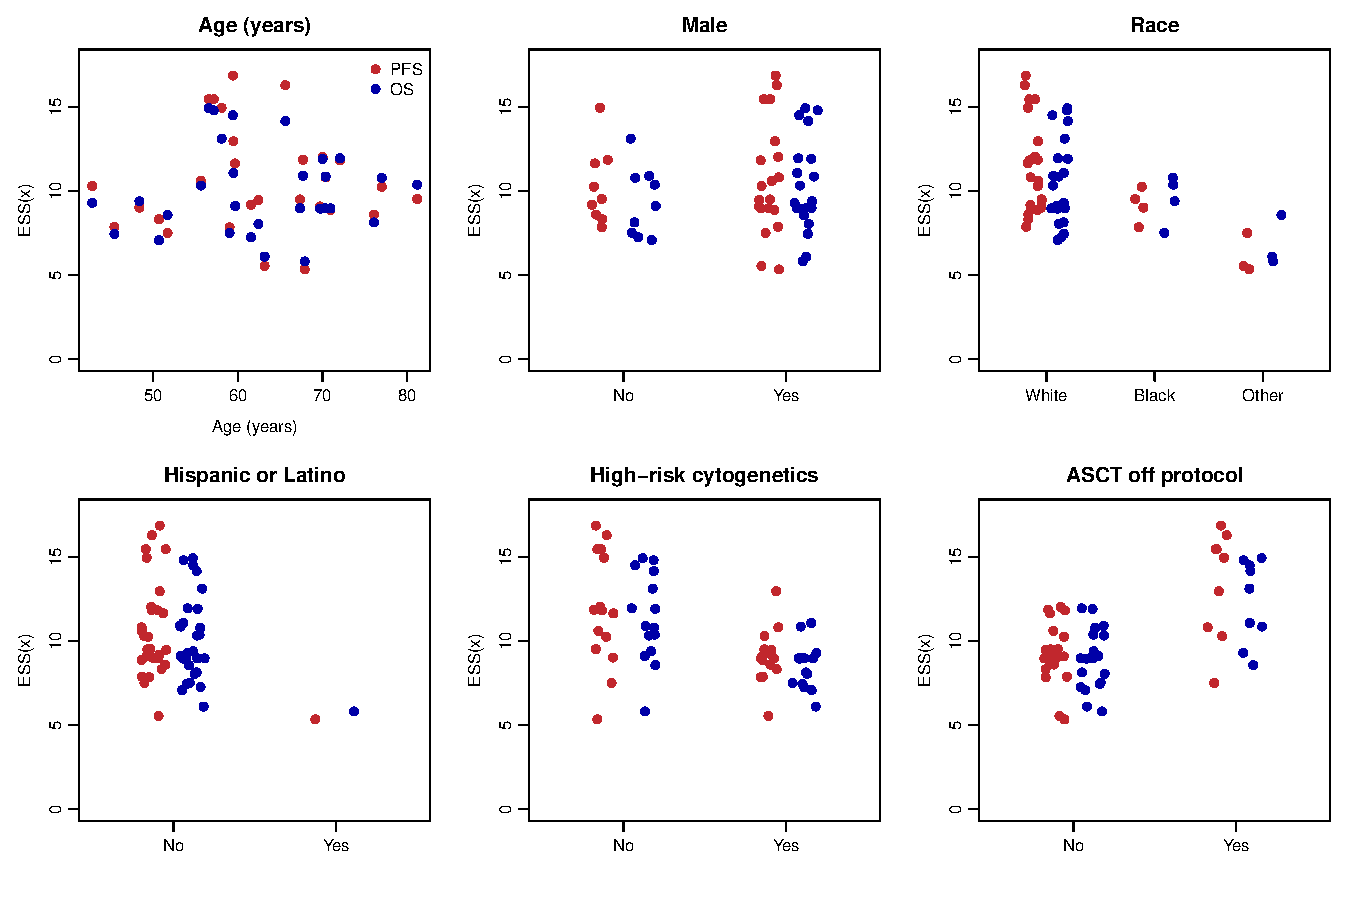
\includegraphics[width=\textwidth]{figures/fig_ess_map.pdf}
\caption{Local prior effective sample size $\mathrm{ESS}(x)=\sigma_1^2/\{V_f(x)+H_g\tau_0^2\}$ at the $30$ EloKRd profiles for PFS (red) and OS (blue) at $N_{\rm target}=30$, plotted against each harmonized covariate; $V_f(x)$ is the UCMM posterior variance of the log-time surface at $x$.}
\label{fig:essmap}
\end{figure}

%==============================================================================
\section{Discussion}
\label{sec:discussion}
%==============================================================================

\DIFdelbegin \DIFdel{The simulations place the method between two familiar ones. The free-offset model, BART with the source as a covariate, is safe everywhere and never gains from agreement, and complete pooling gains from agreement and fails under any disagreement. }\DIFdelend LRC-BART \DIFdelbegin \DIFdel{gains }\DIFdelend \DIFaddbegin \DIFadd{combines an efficiency gain under agreement with a covariate-resolved assessment of compatibility. In the Gaussian simulations, its RMSE is }\DIFaddend about $16\%$ \DIFdelbegin \DIFdel{in RMSE over the free-offset model when the sources agree, abstains at a bias of }\DIFdelend \DIFaddbegin \DIFadd{lower than BART-PP's under Sc1. Under global disagreement, its residual bias is }\DIFaddend about $0.04$\DIFdelbegin \DIFdel{when they disagree everywhere, and finds a regional disagreement }\DIFdelend \DIFaddbegin \DIFadd{. For a regional shift }\DIFaddend of $1.3$ residual SDs, \DIFdelbegin \DIFdel{with a transition of }\DIFdelend \DIFaddbegin \DIFadd{the compatibility map and realized regional ESS distinguish the two regions, although the transition spans }\DIFaddend about one unit of the splitting covariate\DIFdelbegin \DIFdel{around the boundary that we could not remove by tuning and that comes from learning the boundaryfrom about a hundred RCT controls}\DIFdelend \DIFaddbegin \DIFadd{. The control-surface RMSE remains higher than BART-PP's, including away from the boundary}\DIFaddend . At a regional shift of \DIFdelbegin \DIFdel{one residual SDit borrows across the boundary and pays a }\DIFdelend \DIFaddbegin \DIFadd{two thirds of a residual SD, excessive borrowing produces }\DIFaddend bias of $0.04$ and \DIFdelbegin \DIFdel{a }\DIFdelend coverage of $0.89$\DIFdelbegin \DIFdel{, which is the resolution of }\DIFdelend \DIFaddbegin \DIFadd{. The leaf calculation in }\DIFaddend Theorem~\ref{thm:map}(a) \DIFdelbegin \DIFdel{and argues for reporting the map with the estimate rather than for a smaller spike, which would forgo the gain under agreement}\DIFdelend \DIFaddbegin \DIFadd{describes the dependence of detection on the spike scale and local sample size; it does not establish the performance of the full fitted ensemble.
}

\DIFadd{The CAHB comparison illustrates the difficulty of kernel-local borrowing in our nonlinear ten-covariate design. It also depends on our choices for smoothing, precision scaling and joint posterior draws. We therefore interpret it as an assessment of this transfer of CAHB, with the variants reported alongside it}\DIFaddend . The survival study \DIFdelbegin \DIFdel{adds that the median ratio is a poor estimand }\DIFdelend \DIFaddbegin \DIFadd{shows a further limitation: }\DIFaddend with $75$ controls and censoring, \DIFdelbegin \DIFdel{and that }\DIFdelend \DIFaddbegin \DIFadd{the median ratio can amplify control-surface bias and posterior uncertainty. We report }\DIFaddend the RMST ratio \DIFdelbegin \DIFdel{should be reported }\DIFdelend with it. In \DIFdelbegin \DIFdel{the }\DIFdelend \DIFaddbegin \DIFadd{a }\DIFaddend single-arm study, \DIFdelbegin \DIFdel{measured confounding without an internal control biases every method, since nothing in the data can reveal a discrepancy at profiles the external source does not cover; what the calibration contributes there is the ceiling and the local ESS map, which report how thin the external support is at the trial profilesand, in the application, exposed a coding error in the data}\DIFdelend \DIFaddbegin \DIFadd{trial data cannot identify a control discrepancy. The ceiling and local prior ESS then describe external support at trial profiles, but cannot demonstrate compatibility with an unobserved trial control surface}\DIFaddend .

\DIFdelbegin \DIFdel{Several limitations remain. The map results are conditional on the partitions of the discrepancy ensemble and on the true discrepancy being representable on }\DIFdelend \DIFaddbegin \DIFadd{The theoretical results condition on features that are learned in the fitted model. Map consistency requires fixed discrepancy partitions and a true discrepancy in }\DIFaddend their additive span\DIFdelbegin \DIFdel{, and we have no statement about }\DIFdelend \DIFaddbegin \DIFadd{. We have no corresponding result for }\DIFaddend the posterior over partitions\DIFdelbegin \DIFdel{; the leaf results treat the pooled surface as fixed, and with }\DIFdelend \DIFaddbegin \DIFadd{. The leaf-level influence bound also treats }\DIFaddend $f$ \DIFdelbegin \DIFdel{estimated the RWD posterior error at the RCT profiles enters a }\DIFdelend \DIFaddbegin \DIFadd{as fixed; uncertainty in the fitted pooled surface perturbs the residuals used to estimate }\DIFaddend $g$\DIFdelbegin \DIFdel{leaf as a perturbation of the discrepancy. Both are open, and the second is where the boundary leak lives.
}\DIFdelend \DIFaddbegin \DIFadd{. These limitations prevent a direct extension of the conditional results to the full posterior. The observed surface loss under Sc4 remains an empirical limitation even when profiles near the boundary are excluded.
}

\DIFaddend The spike scale is global\DIFdelbegin \DIFdel{and the locality is carried }\DIFdelend \DIFaddbegin \DIFadd{, with locality determined }\DIFaddend by the indicators\DIFdelbegin \DIFdel{; a leaf-specific scale would let compatible regions differ in how compatible they are}\DIFdelend \DIFaddbegin \DIFadd{. Leaf-specific scales could accommodate different degrees of compatibility}\DIFaddend , at the cost of the Inv-$\chi^2$ conjugacy. \DIFdelbegin \DIFdel{The model handles one external source; with several, a discrepancy ensemble per source with a common $w$ is the natural extension, and the ceiling would then be a sum over sources of the information each carries at the RCT profiles}\DIFdelend \DIFaddbegin \DIFadd{Multiple external sources would require source-specific discrepancies and a joint calibration that accounts for their information at the trial profiles; additivity of the ceilings has not been established}\DIFaddend . Binary and count outcomes \DIFdelbegin \DIFdel{need a latent-variable likelihoodin place of the Gaussian one, and the AFT model can be replaced by }\DIFdelend \DIFaddbegin \DIFadd{require an alternative likelihood, and }\DIFaddend a nonparametric survival \DIFdelbegin \DIFdel{BART at the cost of the closed-form RMST . Finally, the calibration sets a prior effective sample size, not an operating characteristic; embedding it in a design that fixes the }\DIFdelend \DIFaddbegin \DIFadd{model would require a different RMST calculation. Prior-ESS calibration alone does not control }\DIFaddend Type I error \DIFdelbegin \DIFdel{rate and the powerunder an agreed mechanism, with the map as a pre-specified diagnostic, is the step that would take the method into a confirmatory setting}\DIFdelend \DIFaddbegin \DIFadd{or power. A confirmatory design would need to evaluate those operating characteristics under specified scenarios and pre-specify how the compatibility map would be used}\DIFaddend .

\bibliographystyle{plainnat}
\bibliography{merged}
\clearpage
\appendix
\begin{center}{\Large Web Appendices}\end{center}
\DIFaddbegin {\emergencystretch=2em
\DIFaddend % appendix_new.tex : theory appendix for LRC-BART (locally robust commensurate BART).
% Standalone body: compile by \input-ing this file into a wrapper that carries the
% preamble of paper/main.tex (see 03-theory/build/wrapper.tex). No \documentclass here.
%
% Bibliography keys used below exist in paper/ref.bib except the two flagged in
% comments (Hahn, Murray and Carvalho 2020; Hobbs et al. 2011), which are cited in
% text only until the entries are added.

% ---- Appendix-local theorem environments (Theorem A1, Lemma A1, ...) -------------
\newtheorem{thmA}{Theorem}
\renewcommand{\thethmA}{A\arabic{thmA}}
\newtheorem{lemA}{Lemma}
\renewcommand{\thelemA}{A\arabic{lemA}}
\newtheorem{propA}{Proposition}
\renewcommand{\thepropA}{A\arabic{propA}}
\newtheorem{corA}{Corollary}
\renewcommand{\thecorA}{A\arabic{corA}}
\theoremstyle{definition}
\newtheorem{assA}{Assumption}
\renewcommand{\theassA}{A\arabic{assA}}
\newtheorem{remA}{Remark}
\renewcommand{\theremA}{A\arabic{remA}}
\theoremstyle{plain}
\renewcommand{\theequation}{A\arabic{equation}}
\newcommand{\Pspike}{P_{\mathrm{spike}}}
\newcommand{\ess}{\mathrm{ESS}}
\newcommand{\Phibar}{\bar\Phi}
\newcommand{\tr}{^{\top}}

\section*{Web Appendix A: Model, notation, and exact leaf marginals}

This appendix collects the proofs for the locally robust commensurate BART (LRC-BART) model of the main text. We fix notation first. The two control sources are indexed by $g=1$ (RCT control) and $g=2$ (RWD control), with residual variances $\sigma_1^2$ and $\sigma_2^2$. The control outcomes follow
\begin{equation}
y_i=f(x_i)+D_i\,g(x_i)+\varepsilon_i,\qquad \varepsilon_i\sim\Normal(0,\sigma^2_{g_i}),\qquad D_i=\mathbf 1\{i\ \text{is an RCT control}\},
\label{eqA:model}
\end{equation}
where $f$ is a standard BART ensemble of $H_f$ trees with leaf prior $\Normal(0,\lambda_f^2)$ and $g$ is an ensemble of $H_g$ trees whose leaves carry the two-component prior
\begin{equation}
\theta_{h\ell}\given z_{h\ell}\sim z_{h\ell}\,\Normal(0,\tau_0^2)+(1-z_{h\ell})\,\Normal(0,\tau_1^2),\qquad z_{h\ell}\iid\Ber(w),
\label{eqA:leafprior}
\end{equation}
with $z=1$ the spike (commensurate component) and $z=0$ the slab, $w\sim\mathrm{Beta}(a_w,b_w)$, $\tau_1^2$ fixed by the range rule, and
\begin{equation}
\tau_0^2\sim\text{scaled-Inv-}\chi^2(\nu_0,s_0^2)\ \text{truncated to }(0,\tau_1^2),
\label{eq:tau0prior}
\end{equation}
which is the prior the sampler implements (its conditional for $\tau_0^2$ is the scaled-Inv-$\chi^2(\nu_0+K_0,\cdot)$ law truncated to $(0,\tau_1^2)$, which is conjugate for \eqref{eq:tau0prior} and not for the untruncated prior). Throughout we impose
\begin{assA}[(A1)]\label{ass:A1}
$0<\tau_0^2<\tau_1^2<\infty$.
\end{assA}
\noindent Under \eqref{eq:tau0prior}, Assumption~\ref{ass:A1} holds almost surely under the prior and along the chain. The prior-ESS calculation of Web Appendix~D uses the untruncated scaled-Inv-$\chi^2(\nu_0,s_0^2)$ law, and we say there where truncation matters; at the calibrated $s_0^2$ of order $10^{-3}$ against $\tau_1^2$ of order one the truncated mass $P(\chi^2_{\nu_0}<\nu_0s_0^2/\tau_1^2)$ is of order $10^{-5}$.

Within a leaf, $n_g$ and $\bar y_g$ denote the number and the mean of the source-$g$ partial residuals routed to the leaf, $v_g=\sigma_g^2/n_g$, and $\phi(\cdot;m,V)$ is the $\Normal(m,V)$ density; $\Phi$ is the standard normal distribution function and $\Phibar=1-\Phi$. For a $g$ leaf only RCT controls enter, and we write $\bar y=\bar y_1$, $v=v_1$, $n=n_1$ when no confusion arises. The identity we use repeatedly is the Gaussian product rule
\begin{equation}
\phi(\theta;0,\tau^2)\,\phi(\bar y;\theta,v)=\phi(\bar y;0,\tau^2+v)\,\phi\Bigl(\theta;\tfrac{\tau^2}{\tau^2+v}\bar y,\ \tfrac{\tau^2 v}{\tau^2+v}\Bigr),
\label{eq:gaussprod}
\end{equation}
which follows by completing the square in $\theta$.

\subsection*{A.1 Exact leaf marginals}

\begin{lemA}[Exact leaf marginals]\label{lem:marg}
Fix all trees other than tree $h$, their leaf parameters, the residual variances, $\lambda_f^2$, and $(\tau_0^2,\tau_1^2,w)$.
\begin{enumerate}[label=(\alph*),leftmargin=2.2em]
\item (\emph{$f$ leaf.}) Let $r_i=y_i-f_{-h}(x_i)-D_ig(x_i)$ be the partial residuals of the control observations routed to a leaf of $f$-tree $h$, so that $r_i\given\theta\indep\Normal(\theta,\sigma^2_{g_i})$ and $\theta\sim\Normal(0,\lambda_f^2)$. With $A=n_1/\sigma_1^2+n_2/\sigma_2^2$ and $B=S_1/\sigma_1^2+S_2/\sigma_2^2$, $S_g=\sum_{i:g_i=g}r_i$,
\begin{equation}
\int\prod_i\phi(r_i;\theta,\sigma^2_{g_i})\,\phi(\theta;0,\lambda_f^2)\,\dd\theta
=\Bigl[\prod_i\phi(r_i;0,\sigma^2_{g_i})\Bigr]\,M_f,\qquad
M_f=\frac{\exp\bigl\{\lambda_f^2B^2/\{2(1+\lambda_f^2A)\}\bigr\}}{(1+\lambda_f^2A)^{1/2}}.
\label{eqA:Mf}
\end{equation}
\item (\emph{$g$ leaf.}) Let $r_i=y_i-f(x_i)-g_{-h}(x_i)$ be the partial residuals of the $n_1$ RCT controls routed to a leaf of $g$-tree $h$, with mean $\bar y$. Under the prior \eqref{eqA:leafprior},
\begin{equation}
\sum_{z\in\{0,1\}}P(z)\int\prod_i\phi(r_i;\theta,\sigma_1^2)\,\phi(\theta;0,\tau_z^2)\,\dd\theta
=\Bigl[\prod_i\phi(r_i;0,\sigma_1^2)\Bigr]\,M_g,
\label{eqA:Mg}
\end{equation}
\begin{equation}
M_g=\frac{w\,\phi(\bar y;0,\tau_0^2+v)+(1-w)\,\phi(\bar y;0,\tau_1^2+v)}{\phi(\bar y;0,v)},
\label{eq:Mg2}
\end{equation}
where $\tau_z^2$ denotes $\tau_0^2$ for $z=1$ and $\tau_1^2$ for $z=0$. A leaf with $n_1=0$ has $M_g=1$.
\item (\emph{Leaf conditionals.}) In a $g$ leaf,
\begin{equation}
P(z=1\given\bar y)=\frac{w\,\phi(\bar y;0,\tau_0^2+v)}{w\,\phi(\bar y;0,\tau_0^2+v)+(1-w)\,\phi(\bar y;0,\tau_1^2+v)},\qquad
\theta\given z,\bar y\sim\Normal\Bigl(\frac{\tau_z^2}{\tau_z^2+v}\bar y,\ \frac{\tau_z^2v}{\tau_z^2+v}\Bigr),
\label{eq:leafcond}
\end{equation}
and in an $f$ leaf $\theta\given\cdot\sim\Normal\bigl(\lambda_f^2B/(1+\lambda_f^2A),\ \lambda_f^2/(1+\lambda_f^2A)\bigr)$.
\end{enumerate}
\end{lemA}

\begin{proof}
(a) Expanding $-(r_i-\theta)^2/(2\sigma^2_{g_i})=-r_i^2/(2\sigma^2_{g_i})+r_i\theta/\sigma^2_{g_i}-\theta^2/(2\sigma^2_{g_i})$ and summing over $i$ gives
$\prod_i\phi(r_i;\theta,\sigma^2_{g_i})=\prod_i\phi(r_i;0,\sigma^2_{g_i})\exp(\theta B-\theta^2A/2)$. Multiplying by $\phi(\theta;0,\lambda_f^2)$ and integrating, the exponent is $-\tfrac12(A+\lambda_f^{-2})\theta^2+B\theta$, a Gaussian integral equal to $(2\pi)^{1/2}(A+\lambda_f^{-2})^{-1/2}\exp\{B^2/(2(A+\lambda_f^{-2}))\}$; dividing by the prior normalizing constant $(2\pi\lambda_f^2)^{1/2}$ gives $M_f$. The conditional of $\theta$ is read off the same quadratic form.

(b) With a single source, (a) gives $\prod_i\phi(r_i;\theta,\sigma_1^2)=\prod_i\phi(r_i;0,\sigma_1^2)\exp\{\theta n\bar y/\sigma_1^2-\theta^2n/(2\sigma_1^2)\}$, and the exponential equals $\phi(\bar y;\theta,v)/\phi(\bar y;0,v)$, since $-\{(\bar y-\theta)^2-\bar y^2\}/(2v)=(2\bar y\theta-\theta^2)n/(2\sigma_1^2)$. Hence the likelihood factors as $\prod_i\phi(r_i;0,\sigma_1^2)\times\phi(\bar y;\theta,v)/\phi(\bar y;0,v)$, the sufficiency of $\bar y$. Integrating $\phi(\bar y;\theta,v)$ against $\phi(\theta;0,\tau_z^2)$ by \eqref{eq:gaussprod} gives $\phi(\bar y;0,\tau_z^2+v)$, and the sum over $z$ with weights $w$ and $1-w$ gives $M_g$. When $n_1=0$ the leaf has no likelihood factor and the integral of the prior is one.

(c) By \eqref{eq:gaussprod}, the joint density of $(z,\theta)$ given $\bar y$ is proportional to $P(z)\phi(\bar y;0,\tau_z^2+v)\,\phi(\theta;\tau_z^2\bar y/(\tau_z^2+v),\tau_z^2v/(\tau_z^2+v))$; summing out $\theta$ gives the stated Bernoulli weight and the remaining factor is the stated conditional of $\theta$.
\end{proof}

\begin{propA}[The tree moves target the exact posterior]\label{prop:exact}
Condition on $(\sigma_1^2,\sigma_2^2,\lambda_f^2,\tau_0^2,\tau_1^2,w)$ and on all trees other than $h$ together with their leaf parameters. Let the update of tree $h$ consist of a Metropolis--Hastings step on the partition $T_h$ with grow, prune, and change proposals, acceptance ratio equal to the tree-prior ratio times the proposal ratio times the ratio of products of $M_f$ (for $f$ trees) or $M_g$ (for $g$ trees) over the affected leaves, followed by a draw of the leaf parameters of $T_h$ (and, for a $g$ tree, the indicators) from \eqref{eq:leafcond}. Then the composite update leaves the conditional posterior of $(T_h,\theta_h)$ (resp.\ $(T_h,\theta_h,z_h)$) invariant. Consequently the full sweep, with the conjugate updates of $(\sigma_g^2,\tau_0^2,w)$, the update of $\tau_0^2$ being the truncated conditional under the prior \eqref{eq:tau0prior}, is a partially collapsed Gibbs sampler whose invariant law is the exact joint posterior under \eqref{eqA:leafprior} and \eqref{eq:tau0prior}.
\end{propA}

\begin{proof}
Given the conditioning, the marginal conditional of $T_h$ with the leaf parameters and indicators integrated out is $\pi(T_h)\prod_i\phi(r_i;0,\sigma^2_{g_i})\prod_{\ell\in T_h}M_\ell$ by Lemma~\ref{lem:marg}, where $M_\ell$ is $M_f$ or $M_g$. The partial residuals $r_i$ do not depend on $T_h$, and the observation-level product is over all observations of the tree, so it is the same for the current and the proposed partition and cancels from the Metropolis--Hastings ratio. The stated acceptance ratio is therefore the exact ratio for the collapsed target; for a grow move that splits leaf $P$ into $L$ and $R$, the leaf factor ratio is $M_LM_R/M_P$, and the prune and change ratios follow in the same way. A Metropolis--Hastings kernel with the exact ratio leaves the collapsed conditional invariant. Drawing the leaf parameters (and indicators) from their exact conditional given $T_h$ then yields a draw from the joint conditional of $(T_h,\theta_h,z_h)$, which is the marginal-then-conditional construction of \citet{Chipman2010BART}. The conjugate updates of $\sigma_g^2$, $\tau_0^2$, and $w$ are ordinary Gibbs steps, so the sweep is a partially collapsed Gibbs sampler with the joint posterior as invariant law.
\end{proof}

\begin{remA}[No surrogate is needed]\label{rem:nosurrogate}
Every factor entering a tree move is closed form because, conditionally on $(\tau_0^2,\tau_1^2,w)$, the leaf prior \eqref{eqA:leafprior} is a finite Gaussian mixture, and the Gaussian likelihood integrates against each component in closed form. The previous model placed a leaf-specific discrepancy variance under a scaled-Inv-$\chi^2$ prior and integrated it inside the leaf marginal, which produced an additive scale mixture, $\int\phi(\bar y_1;0,v_1+\tau^2)\phi(\bar y_2;0,v_2+\tau^2)p(\tau^2)\,\dd\tau^2$, with no elementary form; the moment-matched Student-$t$ surrogate and the perturbation bound of the previous Theorem~2 were the response to that integral. In the present model the scale $\tau_0^2$ is a global parameter updated by its own conjugate step, and the local adaptivity is carried by the per-leaf indicator $z$, so the leaf marginal is exact and the tree kernels target the exact posterior (Proposition~\ref{prop:exact}). The surrogate, its error bound, and the compactness assumption that supported it are therefore no longer part of the method; Web Appendix~F lists what is dropped.
\end{remA}

\section*{Web Appendix B: Bounded local influence (T1)}

\subsection*{B.1 A single $g$ leaf}

We fix a $g$ leaf and condition on $f$, on the other $g$ trees, on the partition, and on $(\sigma_1^2,\tau_0^2,\tau_1^2,w)$, so that $\bar y\given\theta\sim\Normal(\theta,v)$ with $v=\sigma_1^2/n$. Write
\begin{equation}
\rho_j=\frac{\tau_j^2}{\tau_j^2+v},\qquad \hat\theta_j=\rho_j\,\bar y,\qquad V_j=\rho_j\,v=\frac{\tau_j^2v}{\tau_j^2+v},\qquad j\in\{0,1\},
\label{eq:rho}
\end{equation}
so that $\hat\theta_1$ is the slab estimate (close to the RCT-only residual mean $\bar y$ when $\tau_1^2\gg v$) and $\hat\theta_0$ the spike-shrunk estimate (close to zero, that is, to the pooled surface $f$, when $\tau_0^2\ll v$). The subscript $j$ of $\rho_j$, $\hat\theta_j$, $V_j$ indexes the scale $\tau_j^2$, so $j=1$ is the slab, whereas the indicator convention of \eqref{eqA:leafprior} has $z=1$ for the spike. Under Assumption~\ref{ass:A1}, $0<\rho_0<\rho_1<1$. Let $p=P(z=0\given\bar y)$ be the posterior slab probability and define
\begin{equation}
\kappa=\frac{1}{2}\Bigl(\frac{1}{\tau_0^2+v}-\frac{1}{\tau_1^2+v}\Bigr),\qquad
a=\log\frac{1-w}{w}+\frac{1}{2}\log\frac{\tau_0^2+v}{\tau_1^2+v},\qquad
C=e^{-a}=\frac{w}{1-w}\sqrt{\frac{\tau_1^2+v}{\tau_0^2+v}}.
\label{eq:kappaC}
\end{equation}
Under Assumption~\ref{ass:A1}, $\kappa>0$, and a direct computation gives
\begin{equation}
\rho_1-\rho_0=\frac{v(\tau_1^2-\tau_0^2)}{(\tau_1^2+v)(\tau_0^2+v)}=2v\kappa .
\label{eq:rhodiff}
\end{equation}

\begin{thmA}[Bounded local influence]\label{thm:T1}
Under Assumption~\ref{ass:A1} and the conditioning above, the following hold for every $\bar y\in\mathbb R$; parts (b) to (d) assume $0<w<1$.
\begin{enumerate}[label=(\alph*),leftmargin=2.2em]
\item (\emph{Posterior.}) $\theta\given\bar y\sim p\,\Normal(\hat\theta_1,V_1)+(1-p)\,\Normal(\hat\theta_0,V_0)$, and hence
\begin{equation}
\E[\theta\given\bar y]=p\,\frac{\tau_1^2}{\tau_1^2+v}\,\bar y+(1-p)\,\frac{\tau_0^2}{\tau_0^2+v}\,\bar y .
\label{eq:postmean}
\end{equation}
\item (\emph{Slab probability.}) $\displaystyle \logit p=\log\frac{p}{1-p}=a+\kappa\,\bar y^2$, with $a$ and $\kappa$ as in \eqref{eq:kappaC}.
\item (\emph{Bounded spike contribution and bounded RWD-induced shift.}) The spike-shrunk part of \eqref{eq:postmean} satisfies $|(1-p)\hat\theta_0|\le|\bar y|\,\tau_0^2/(\tau_0^2+v)$. The shift of the posterior mean relative to the slab estimate,
\begin{equation}
I(\bar y)=\E[\theta\given\bar y]-\hat\theta_1=-(1-p)\,(\rho_1-\rho_0)\,\bar y ,
\label{eq:I}
\end{equation}
satisfies $|I(\bar y)|\le(\rho_1-\rho_0)\,|\bar y|\,\min\{1,\,Ce^{-\kappa\bar y^2}\}$ and
\begin{equation}
\sup_{\bar y\in\mathbb R}|I(\bar y)|\ \le\ 2v\sqrt{\kappa\max\{\log C,\tfrac12\}}\ \le\ \sqrt{2v\max\{\log C,\tfrac12\}} .
\label{eq:supI}
\end{equation}
\item (\emph{Gaussian rate.}) $1-p\le Ce^{-\kappa\bar y^2}$, so $p\to1$ and $I(\bar y)\to0$ as $|\bar y|\to\infty$, at a Gaussian rate.
\item (\emph{Nested cases.}) With $w=1$ (C-BART), $p\equiv0$ and $I(\bar y)=-(\rho_1-\rho_0)\bar y$, linear and unbounded; if in addition $\tau_0^2\to0$ (BART-CP), $\E[\theta\given\bar y]\to0$ and $I(\bar y)\to-\rho_1\bar y$. With $w=0$, $p\equiv1$ and $I\equiv0$. If Assumption~\ref{ass:A1} fails with $\tau_0^2>\tau_1^2$, then $\kappa<0$, the roles of the two components are exchanged, and (c), (d) hold with the wide component in the role of the slab; if $\tau_0^2=\tau_1^2$, $p\equiv1-w$ and $I\equiv0$.
\end{enumerate}
\end{thmA}

\begin{proof}
(a) The posterior density is proportional to $\{w\phi(\theta;0,\tau_0^2)+(1-w)\phi(\theta;0,\tau_1^2)\}\phi(\bar y;\theta,v)$. Applying \eqref{eq:gaussprod} to each term gives $w\phi(\bar y;0,\tau_0^2+v)\phi(\theta;\hat\theta_0,V_0)+(1-w)\phi(\bar y;0,\tau_1^2+v)\phi(\theta;\hat\theta_1,V_1)$, a two-component Gaussian mixture with weights proportional to $w\phi(\bar y;0,\tau_0^2+v)$ and $(1-w)\phi(\bar y;0,\tau_1^2+v)$; normalizing gives $1-p$ and $p$ as in \eqref{eq:leafcond}, and \eqref{eq:postmean} is the mean of the mixture.

(b) The log odds of the two weights are
\[
\log\frac{(1-w)\phi(\bar y;0,\tau_1^2+v)}{w\,\phi(\bar y;0,\tau_0^2+v)}
=\log\frac{1-w}{w}-\frac{1}{2}\log\frac{\tau_1^2+v}{\tau_0^2+v}+\frac{\bar y^2}{2}\Bigl(\frac{1}{\tau_0^2+v}-\frac{1}{\tau_1^2+v}\Bigr)=a+\kappa\bar y^2 .
\]

(c) The first bound is immediate from $0\le1-p\le1$. For $I$, subtract $\hat\theta_1$ from \eqref{eq:postmean}. Since $1-p=(1+e^{a+\kappa\bar y^2})^{-1}\le\min\{1,e^{-a-\kappa\bar y^2}\}=\min\{1,Ce^{-\kappa\bar y^2}\}$, the pointwise bound follows. For the supremum we show that for $\kappa>0$ and $C>0$,
\begin{equation}
\sup_{u\in\mathbb R}|u|\min\{1,Ce^{-\kappa u^2}\}\le\sqrt{\max\{\log C,\tfrac12\}/\kappa}.
\label{eq:sup-lemma}
\end{equation}
Put $t=\kappa u^2$. On $\{t\le\log C\}$ (empty if $C\le1$) the left side is at most $|u|\le\sqrt{\log C/\kappa}$. On $\{t>\max(\log C,0)\}$ the left side equals $\sqrt{t/\kappa}\,Ce^{-t}$. If $\log C\ge\tfrac12$, the function $\sqrt t\,e^{-t}$ is decreasing on $[\tfrac12,\infty)$, so the value is at most $\sqrt{\log C/\kappa}\,Ce^{-\log C}=\sqrt{\log C/\kappa}$. If $\log C<\tfrac12$, then $\sup_{t>0}\sqrt t\,e^{-t}=(2e)^{-1/2}$ gives at most $C(2e\kappa)^{-1/2}<\sqrt{1/(2\kappa)}$ because $C<e^{1/2}$. This proves \eqref{eq:sup-lemma}. Combining with \eqref{eq:rhodiff}, $\sup|I|\le2v\kappa\sqrt{\max\{\log C,\tfrac12\}/\kappa}=2v\sqrt{\kappa\max\{\log C,\tfrac12\}}$, and $\kappa\le1/(2(\tau_0^2+v))\le1/(2v)$ gives the second inequality in \eqref{eq:supI}.

(d) is the pointwise bound in (c) together with $\kappa>0$. (e) With $w=1$ the slab weight is zero for every $\bar y$; with $w=0$ the spike weight is zero; the remaining statements are read off \eqref{eq:kappaC} and \eqref{eq:I}.
\end{proof}

\begin{remA}[What is and is not bounded]\label{rem:slabshrink}
Theorem~\ref{thm:T1} bounds the influence of the commensurate component relative to the slab estimate $\hat\theta_1=\rho_1\bar y$. The slab estimate itself is shrunk toward zero, that is toward the pooled surface $f$, by the factor $\rho_1$: $\E[\theta\given\bar y]-\bar y=-(1-\rho_1)\bar y+I(\bar y)$ with $1-\rho_1=v/(\tau_1^2+v)$. This linear term is the range-rule regularization that any BART leaf with prior variance $\tau_1^2$ applies, and it is of the same form as the shrinkage of a BART-NP leaf toward its ensemble center; at $n=50$, $\sigma_1=1.5$ and $\tau_1^2=1.25$ its slope is $0.035$. The bounded term $I$ is the part specific to borrowing.
\end{remA}

\begin{remA}[Numerical illustration]\label{rem:T1num}
With $\sigma_1=1.5$, $n=50$, $\tau_0^2=0.001$ (the scale calibrated for $N_{\rm target}=100$ in the Gaussian study), $\tau_1^2=1.25$ (the range rule at $H_g=5$ for an outcome range of $10$) and $w=0.8$ fixed for illustration, $v=0.045$, $\kappa=10.5$, $C=21.2$, $\log C=3.06$, and $\rho_1-\rho_0=0.94$. The bound \eqref{eq:supI} gives $\sup|I|\le0.51$; the exact supremum of \eqref{eq:I}, a one-dimensional maximization, is $0.31$, attained at $\bar y=0.43$. By comparison C-BART's shift is $0.94\,|\bar y|$, which exceeds $0.51$ once $|\bar y|>0.54$.
\end{remA}

\subsection*{B.2 The estimand level: fixed partitions of the $g$ ensemble}

The estimand is the RCT-standardized control mean $\mu=N^{-1}\sum_{i\le N}f_1(x_i)$ over the $N$ RCT covariate profiles, and $f_1=f+g$, so $\mu=\mu_f+\mu_g$ with $\mu_g=N^{-1}\sum_{i\le N}g(x_i)$. We condition on $f$, on the partitions $\mathcal T=(T_1,\dots,T_{H_g})$ of the $g$ trees, and on $(\sigma_1^2,\tau_0^2,\tau_1^2,w)$; the RWD then enters $\mu_g$ only through the shrinkage of $g$ toward zero. Index the $L_g$ leaves of all $g$ trees by $j$, let $\theta\in\mathbb R^{L_g}$ collect the leaf parameters and $z\in\{0,1\}^{L_g}$ the indicators, and let $r\in\mathbb R^{n_1}$ be the residuals $y_i-f(x_i)$ of the RCT controls. Let $X\in\{0,1\}^{n_1\times L_g}$ be the incidence matrix ($X_{ij}=1$ if control $i$ falls in leaf $j$), so each row of $X$ has exactly $H_g$ ones and $g(x_i)=(X\theta)_i$. Let $a\in\mathbb R^{L_g}$ with $a_j=N_j/N$, $N_j$ the number of estimand profiles in leaf $j$, so $\mu_g=a\tr\theta$, $\|a\|_1=H_g$, and $\|a\|_2^2\le\max_ja_j\sum_ja_j\le H_g$, so $\|a\|_2\le\sqrt{H_g}$. Then
\begin{equation}
r\given\theta\sim\Normal(X\theta,\sigma_1^2I),\qquad \theta\given z\sim\Normal(0,D_z),\quad D_z=\mathrm{diag}(\tau^2_{z_j}),\qquad \pi(z)=\prod_jw^{z_j}(1-w)^{1-z_j}.
\label{eq:linform}
\end{equation}
Standard Gaussian algebra gives, with $V_z=XD_zX\tr+\sigma_1^2I$ and $\Sigma_z=(X\tr X/\sigma_1^2+D_z^{-1})^{-1}$,
\begin{equation}
P(z\given r)\propto\pi(z)\,\phi_{n_1}(r;0,V_z),\qquad
\theta\given z,r\sim\Normal\bigl(\hat\theta(z),\Sigma_z\bigr),\qquad \hat\theta(z)=D_zX\tr V_z^{-1}r,
\label{eqA:zpost}
\end{equation}
where the form of $\hat\theta(z)$ follows from $(X\tr X/\sigma^2+D^{-1})^{-1}X\tr/\sigma^2=DX\tr(XDX\tr+\sigma^2I)^{-1}$. We write $\mathbf 0$ for the all-slab configuration; the $w=0$ model (the tree analogue of BART-PP, a free source offset regularized by the range rule) has $\E_{w=0}[\mu_g\given r]=a\tr\hat\theta(\mathbf 0)$, and we call
\begin{equation}
\Delta(r)=\E[\mu_g\given r]-a\tr\hat\theta(\mathbf 0)=\sum_{z\ne\mathbf 0}P(z\given r)\,a\tr\bigl(\hat\theta(z)-\hat\theta(\mathbf 0)\bigr)
\label{eq:Delta}
\end{equation}
the RWD-induced shift of the estimand at the given partitions.

\begin{corA}[Bounded shift of the standardized control mean]\label{cor:estimand}
Under Assumption~\ref{ass:A1}, $0<w<1$, and the conditioning of this subsection, let $\delta=\tau_1^2-\tau_0^2$ and $b=w\tau_1/\{(1-w)\tau_0\}$.
\begin{enumerate}[label=(\alph*),leftmargin=2.2em]
\item (\emph{General partitions.}) $\displaystyle\sup_{r\in\mathbb R^{n_1}}|\Delta(r)|\le \sqrt{H_g}\Bigl(1+\frac{\tau_1}{\tau_0}\Bigr)(2^{L_g}-1)\sqrt{2\delta\max\{L_g\log b,\tfrac12\}}<\infty$.
\item (\emph{Single tree, $H_g=1$.}) With leaves $\ell$, RCT counts $n_{1\ell}$, $v_\ell=\sigma_1^2/n_{1\ell}$, leaf means $\bar y_\ell$, and $\kappa_\ell,C_\ell$ as in \eqref{eq:kappaC} with $v=v_\ell$,
\[
\Delta(r)=\sum_{\ell:\,n_{1\ell}>0}a_\ell\,I_\ell(\bar y_\ell),\qquad
\sup_r|\Delta(r)|\le\sum_\ell a_\ell\sqrt{2v_\ell\max\{\log C_\ell,\tfrac12\}} ,
\]
and the right side is at most $\max_\ell\sqrt{2v_\ell\max\{\log C_\ell,\tfrac12\}}$.
\item (\emph{$H_g$ trees with a common partition.}) If all $g$ trees share one partition with leaves $\ell$, write $\vartheta_\ell=\sum_h\theta_{h\ell}$, $T_k=k\tau_0^2+(H_g-k)\tau_1^2$, $\rho^{(k)}_\ell=T_k/(T_k+v_\ell)$,
\[
\kappa_{k\ell}=\frac{1}{2}\Bigl(\frac{1}{T_k+v_\ell}-\frac{1}{T_0+v_\ell}\Bigr),\qquad
C_{k\ell}=\binom{H_g}{k}\Bigl(\frac{w}{1-w}\Bigr)^{k}\sqrt{\frac{T_0+v_\ell}{T_k+v_\ell}} .
\]
Then $P(k\ \text{spikes in leaf }\ell\given\bar y_\ell)\propto\binom{H_g}{k}w^k(1-w)^{H_g-k}\phi(\bar y_\ell;0,T_k+v_\ell)$, the leaves are independent a posteriori,
\begin{align}
\Delta(r)&=-\sum_\ell a_\ell\,\bar y_\ell\sum_{k=1}^{H_g}P(k\given\bar y_\ell)\bigl(\rho^{(0)}_\ell-\rho^{(k)}_\ell\bigr),
\label{eq:Delta-common}\\
\sup_r|\Delta(r)|&\le\max_\ell\ 2v_\ell\sum_{k=1}^{H_g}\sqrt{\kappa_{k\ell}\max\{\log C_{k\ell},\tfrac12\}}
\ \le\ \max_\ell H_g\,v_\ell\sqrt{\frac{2\max_k\max\{\log C_{k\ell},\tfrac12\}}{H_g\tau_0^2+v_\ell}} .
\label{eq:Delta-common-bound}
\end{align}
\item (\emph{Contrasts.}) Under complete pooling of the control surface ($w=1$, $\tau_0^2\to0$) the shift is $-a\tr\hat\theta(\mathbf 0)$, and under C-BART ($w=1$) it is $a\tr(\hat\theta(\mathbf 1)-\hat\theta(\mathbf 0))$; both are linear in $r$, and each is unbounded on $\mathbb R^{n_1}$ unless the corresponding linear functional vanishes identically. For a single tree the C-BART functional is $-\sum_\ell a_\ell(\rho_{1\ell}-\rho_{0\ell})\bar y_\ell$, which is nonzero whenever some leaf has $a_\ell>0$ and $n_{1\ell}>0$.
\end{enumerate}
\end{corA}

\begin{proof}
(a) Fix $z\ne\mathbf 0$, let $S=\{j:z_j=1\}$ be its spike leaves, $E_S$ the diagonal indicator of $S$, $X_S$ the corresponding columns of $X$, and $u=X_S\tr V_{\mathbf 0}^{-1}r\in\mathbb R^{|S|}$. Since $D_{\mathbf 0}-D_z=\delta E_S$,
\[
V_z^{-1}-V_{\mathbf 0}^{-1}=V_z^{-1}(V_{\mathbf 0}-V_z)V_{\mathbf 0}^{-1}=\delta\,V_z^{-1}X_SX_S\tr V_{\mathbf 0}^{-1},
\qquad\text{so}\qquad
V_z^{-1}r=V_{\mathbf 0}^{-1}r+\delta\,V_z^{-1}X_Su .
\]
Three consequences follow. First, the quadratic form in the likelihood ratio is
\[
r\tr(V_z^{-1}-V_{\mathbf 0}^{-1})r=\delta\,(V_z^{-1}r)\tr X_Su=\delta\bigl(u+\delta X_S\tr V_z^{-1}X_Su\bigr)\tr u=\delta\|u\|^2+\delta^2u\tr X_S\tr V_z^{-1}X_Su\ \ge\ \delta\|u\|^2 .
\]
Second, the difference of posterior means is
\[
\hat\theta(z)-\hat\theta(\mathbf 0)=(D_z-D_{\mathbf 0})X\tr V_{\mathbf 0}^{-1}r+D_zX\tr(V_z^{-1}-V_{\mathbf 0}^{-1})r=-\delta\,\iota_Su+\delta\,D_zX\tr V_z^{-1}X_S\,u ,
\]
where $\iota_S$ embeds $\mathbb R^{|S|}$ into the $S$ coordinates of $\mathbb R^{L_g}$. The matrix $D_zX\tr V_z^{-1}X=D_z^{1/2}\{M\tr(MM\tr+\sigma_1^2I)^{-1}M\}D_z^{-1/2}$ with $M=XD_z^{1/2}$, and the bracket is symmetric with eigenvalues $\lambda_i/(\lambda_i+\sigma_1^2)\in[0,1)$, so $\|D_zX\tr V_z^{-1}X_S\|\le\|D_zX\tr V_z^{-1}X\|\le\|D_z^{1/2}\|\|D_z^{-1/2}\|\le\tau_1/\tau_0$, and $\|\hat\theta(z)-\hat\theta(\mathbf 0)\|\le\delta(1+\tau_1/\tau_0)\|u\|$. Third, $|V_z|=\sigma_1^{2n_1}|D_z|\,|D_z^{-1}+X\tr X/\sigma_1^2|$ and $D_z^{-1}\succeq D_{\mathbf 0}^{-1}$ give $|V_{\mathbf 0}|/|V_z|\le|D_{\mathbf 0}|/|D_z|=(\tau_1^2/\tau_0^2)^{|S|}$, so
\begin{align*}
P(z\given r)\le\frac{P(z\given r)}{P(\mathbf 0\given r)}
&=\frac{\pi(z)}{\pi(\mathbf 0)}\sqrt{\frac{|V_{\mathbf 0}|}{|V_z|}}\exp\Bigl\{-\tfrac12r\tr(V_z^{-1}-V_{\mathbf 0}^{-1})r\Bigr\}\\
&\le c_z\,e^{-\delta\|u\|^2/2},\qquad c_z=b^{|S|}.
\end{align*}
Combining, and using \eqref{eq:sup-lemma} in the variable $\|u\|$ with $\kappa=\delta/2$,
\begin{align*}
\bigl|P(z\given r)\,a\tr(\hat\theta(z)-\hat\theta(\mathbf 0))\bigr|
&\le\|a\|\,\delta\Bigl(1+\frac{\tau_1}{\tau_0}\Bigr)\|u\|\min\{1,c_ze^{-\delta\|u\|^2/2}\}\\
&\le \sqrt{H_g}\Bigl(1+\frac{\tau_1}{\tau_0}\Bigr)\sqrt{2\delta\max\{|S|\log b,\tfrac12\}} .
\end{align*}
Summing over the $2^{L_g}-1$ configurations $z\ne\mathbf 0$ and using $|S|\le L_g$ gives (a).

(b) For a single tree $X\tr X$ is diagonal, the residual vector splits by leaf, and \eqref{eq:linform} factorizes over leaves, so the leaves are independent a posteriori and each is the single-leaf model of Section~B.1 with $v=v_\ell$; leaves with $n_{1\ell}=0$ have posterior equal to prior under every $w$ and contribute zero to $\Delta$. Theorem~\ref{thm:T1}(c) bounds each $|I_\ell|$, and $\sum_\ell a_\ell=1$ gives the last inequality.

(c) With a common partition, the residual in leaf $\ell$ is $r_i=\vartheta_\ell+\varepsilon_i$ and, given the indicators, $\vartheta_\ell\sim\Normal(0,T_{k_\ell})$ with $k_\ell$ the number of spikes among the $H_g$ leaves stacked on $\ell$; the leaves are independent a posteriori and $\mu_g=\sum_\ell a_\ell\vartheta_\ell$. Summing $\pi(z)\phi(\bar y_\ell;0,T_k+v_\ell)$ over the $\binom{H_g}{k}$ configurations with $k$ spikes gives the stated posterior of $k$, and \eqref{eq:gaussprod} gives $\E[\vartheta_\ell\given k,\bar y_\ell]=\rho^{(k)}_\ell\bar y_\ell$. Under $w=0$, $k=0$ almost surely, which gives the expression for $\Delta$. For $k\ge1$, $P(k\given\bar y_\ell)\le P(k\given\bar y_\ell)/P(0\given\bar y_\ell)=C_{k\ell}e^{-\kappa_{k\ell}\bar y_\ell^2}$, and $\rho^{(0)}_\ell-\rho^{(k)}_\ell=v_\ell(T_0-T_k)/\{(T_0+v_\ell)(T_k+v_\ell)\}=2v_\ell\kappa_{k\ell}$; the $k$-th term is therefore at most $2v_\ell\kappa_{k\ell}|\bar y_\ell|\min\{1,C_{k\ell}e^{-\kappa_{k\ell}\bar y_\ell^2}\}\le2v_\ell\sqrt{\kappa_{k\ell}\max\{\log C_{k\ell},\tfrac12\}}$ by \eqref{eq:sup-lemma}. The final form uses $\kappa_{k\ell}\le\kappa_{H_g\ell}\le1/\{2(H_g\tau_0^2+v_\ell)\}$ and $\sum_\ell a_\ell=1$.

(d) With $w=1$ the posterior over $z$ is degenerate at $\mathbf 1$, so $\E[\mu_g\given r]=a\tr\hat\theta(\mathbf 1)$, linear in $r$; as $\tau_0^2\to0$, $\hat\theta(\mathbf 1)\to0$. A nonzero linear functional on $\mathbb R^{n_1}$ is unbounded. For a single tree, $\hat\theta_\ell(\mathbf 1)-\hat\theta_\ell(\mathbf 0)=(\rho_{0\ell}-\rho_{1\ell})\bar y_\ell$ by (b).
\end{proof}

\begin{remA}[On the constants]\label{rem:constants}
The constant in (a) is finite for every design and every partition, which is the content of the statement, but it is far from sharp: it treats each of the $2^{L_g}-1$ non-slab configurations separately and bounds the posterior probability of each by its odds against the all-slab configuration. Parts (b) and (c) are the cases in which the sum collapses, and they display the dependence on $H_g$, on $\tau_0$ through $\kappa$, and on the leaf shrinkage $\rho^{(H_g)}_\ell=H_g\tau_0^2/(H_g\tau_0^2+v_\ell)$ of the all-spike state. For the numbers of Remark~\ref{rem:T1num} with $\tau_0^2=0.0012$ and the study's configuration $H_g=5$, the common-partition bound in (c) is $1.15$ per leaf, while the exact supremum of \eqref{eq:Delta-common} is $0.148$, attained at $\bar y_\ell=0.33$ (at $H_g=10$ the corresponding values are $1.80$ and $0.067$ at $0.30$); the ensemble abstains sooner than a single leaf because there are $H_g$ ways to place one slab, and one slab leaf absorbs almost all of the discrepancy. The exact supremum is a one-dimensional maximization and is what we recommend reporting.
\end{remA}

\section*{Web Appendix C: Detection and the borrowing map (T2)}

\subsection*{C.1 A single $g$ leaf under a true local shift}

We keep the conditioning of Section~B.1 and add a data-generating assumption: the RCT residuals in the leaf are $r_i=d+\epsilon_i$ with $\epsilon_i\iid\Normal(0,\sigma_1^2)$, where $d$ is the true local discrepancy between the RCT control surface and the pooled surface $f$ (taken as fixed; see the Gap paragraph in Section~C.3 for the estimated $f$). Then $\bar y\sim\Normal(d,v)$, $v=\sigma_1^2/n$. Let $\Pspike(\bar y)=1-p=P(z=1\given\bar y)$.

\begin{thmA}[Leaf-level detection]\label{thm:T2}
Under Assumption~\ref{ass:A1} and the conditioning above:
\begin{enumerate}[label=(\alph*),leftmargin=2.2em]
\item (\emph{Spike probability.}) $\Pspike(\bar y)=\{1+\exp(a+\kappa\bar y^2)\}^{-1}$ with $a,\kappa$ as in \eqref{eq:kappaC}; it depends on $(\bar y,n)$ only through $\bar y^2$ and $v=\sigma_1^2/n$, is decreasing in $|\bar y|$, and satisfies $\Pspike(0)=\{1+e^{a}\}^{-1}$.
\item (\emph{Half-detection discrepancy.}) If $\log\frac{w}{1-w}+\frac{1}{2}\log\frac{\tau_1^2+v}{\tau_0^2+v}>0$, the equation $\Pspike(\bar y)=\tfrac12$ has the unique positive solution
\begin{equation}
d_{1/2}=\sqrt{\frac{2(\tau_0^2+v)(\tau_1^2+v)}{\tau_1^2-\tau_0^2}\Bigl\{\log\frac{w}{1-w}+\frac{1}{2}\log\frac{\tau_1^2+v}{\tau_0^2+v}\Bigr\}}\ ;
\label{eq:dhalf}
\end{equation}
otherwise $\Pspike\le\tfrac12$ for every $\bar y$ (with equality only at $\bar y=0$ when the bracket vanishes) and we set $d_{1/2}=0$. When $\tau_1^2\gg\tau_0^2+v$, $d_{1/2}^2\approx2(\tau_0^2+v)\{\log\frac{w}{1-w}+\frac{1}{2}\log\frac{\tau_1^2}{\tau_0^2+v}\}$, a few multiples of $\tau_0^2+\sigma_1^2/n$. The probability that the leaf's slab probability exceeds one half, under the true shift $d$, is
\begin{equation}
P_d\bigl(p(\bar y)>\tfrac12\bigr)=P_d(|\bar y|>d_{1/2})=\Phibar\Bigl(\frac{d_{1/2}-d}{\sqrt v}\Bigr)+\Phibar\Bigl(\frac{d_{1/2}+d}{\sqrt v}\Bigr).
\label{eq:detectprob}
\end{equation}
\item (\emph{Large $n$, $\tau_0^2$ fixed.}) As $n\to\infty$, almost surely
\begin{equation}
\Pspike(\bar y)\ \to\ \Pspike^\infty(d)=\Bigl\{1+\frac{(1-w)\tau_0}{w\,\tau_1}\exp\Bigl(\frac{d^2}{2}\Bigl(\frac{1}{\tau_0^2}-\frac{1}{\tau_1^2}\Bigr)\Bigr)\Bigr\}^{-1}\in(0,1).
\label{eq:pinf}
\end{equation}
In particular, when $d=0$ (borrowing is warranted), $\Pspike\to w\tau_1/\{w\tau_1+(1-w)\tau_0\}>w$; when $d\ne0$, $\Pspike^\infty(d)\le\frac{w\tau_1}{(1-w)\tau_0}\exp\{-\frac{d^2}{2}(\tau_0^{-2}-\tau_1^{-2})\}$, which tends to zero as $|d|/\tau_0\to\infty$ but is strictly positive for every fixed $d$.
\item (\emph{Large $n$ with a vanishing spike.}) If $\tau_0^2=\tau_{0,n}^2\to0$ as $n\to\infty$ (with $\tau_1^2$, $w$ fixed), then for every $d\ne0$, $\Pspike(\bar y)\to0$ almost surely.
\end{enumerate}
\end{thmA}

\begin{proof}
(a) is Theorem~\ref{thm:T1}(b) with $\kappa>0$. (b) Setting $a+\kappa\bar y^2=0$ gives $\bar y^2=-a/\kappa$, which is \eqref{eq:dhalf} after substituting \eqref{eq:kappaC}; the condition is $-a>0$. The approximation drops $v$ and $\tau_0^2$ against $\tau_1^2$ in $(\tau_1^2+v)/(\tau_1^2-\tau_0^2)$. Since $p>\tfrac12$ iff $|\bar y|>d_{1/2}$ and $\bar y\sim\Normal(d,v)$, \eqref{eq:detectprob} follows.

(c) By the strong law, $\bar y\to d$ almost surely; $v\to0$ gives $a\to a_\infty=\log\frac{1-w}{w}+\frac{1}{2}\log\frac{\tau_0^2}{\tau_1^2}$ and $\kappa\to\kappa_\infty=\frac{1}{2}(\tau_0^{-2}-\tau_1^{-2})$, both finite. Hence $a+\kappa\bar y^2\to a_\infty+\kappa_\infty d^2$ almost surely, and \eqref{eq:pinf} follows by continuity of $t\mapsto(1+e^t)^{-1}$; the limit is strictly between $0$ and $1$ because the exponent is finite. The bound on $\Pspike^\infty(d)$ is $(1+e^t)^{-1}\le e^{-t}$.

(d) Write $\epsilon_n=\tau_{0,n}^2+v_n\to0$. Then $a_n+\kappa_n\bar y_n^2\ge\log\frac{1-w}{w}+\frac{1}{2}\log\frac{\epsilon_n}{\tau_1^2+v_n}+\bar y_n^2\bigl(\frac{1}{2\epsilon_n}-\frac{1}{2\tau_1^2}\bigr)$. Almost surely $\bar y_n^2\to d^2>0$, and $\frac{d^2}{2\epsilon_n}+\frac{1}{2}\log\epsilon_n\to\infty$, so the log odds of the slab diverge and $\Pspike\to0$.
\end{proof}

\paragraph{Gap (consistency of abstention).}
The design specification states that $\Pspike\to0$ as $n\to\infty$ for any nonzero shift. Theorem~\ref{thm:T2}(c) shows this is false for a fixed spike scale: because the spike is a $\Normal(0,\tau_0^2)$ component and not a point mass, a discrepancy of the order of $\tau_0$ is consistent with it, and the limiting spike probability \eqref{eq:pinf} is positive for every $d$. What is true is (i) the limit is exponentially small in $d^2/(2\tau_0^2)$, so abstention is consistent in the regime $|d|/\tau_0\to\infty$, and (ii) abstention is consistent for every fixed $d\ne0$ when the spike scale shrinks with $n$ (part (d)). In the two-arm sampler $\tau_0^2$ is learned from the spike leaves under a prior calibrated to the order $10^{-3}$, so on the outcome scale (i) is the operative statement: at $\tau_0^2=0.001$ a shift of $d=0.5$ has $d^2/(2\tau_0^2)=125$. The consistency statement that does hold for every fixed $d\ne0$, without a vanishing spike, is the one for the discrepancy map in Theorem~\ref{thm:gmap} below.

\begin{remA}[Numerical illustration]\label{rem:T2num}
With the constants of Remark~\ref{rem:T1num}, \eqref{eq:dhalf} gives $d_{1/2}=0.54$ (the specification's rough figure was $0.7$), and \eqref{eq:detectprob} gives leaf abstention probabilities $0.011$, $0.43$, $0.98$ and $1.00$ at true shifts $d=0$, $0.5$, $1$ and $2$. The limit \eqref{eq:pinf} at $d=0$ is $0.993$.
\end{remA}

\subsection*{C.2 The borrowing map $P(|g(x)|<c\given\text{data})$}

The map we display is the posterior probability that the local discrepancy is smaller than a pre-specified outcome-scale threshold $c>0$, $\mathcal B_c(x)=P(|g(x)|<c\given\text{data})$, together with the all-spike map $B(x)=P(\text{all }H_g\text{ leaves covering }x\text{ are spike}\given\text{data})$ as a diagnostic. For a single tree and a fixed partition, $g(x)=\theta_\ell$ for $x$ in leaf $\ell$, and the two are related by the leaf mixture of Theorem~\ref{thm:T1}(a).

\begin{thmA}[The discrepancy map for a single tree]\label{thm:gmap}
Under Assumption~\ref{ass:A1}, for a single $g$ tree with a fixed partition, $f$ and $(\sigma_1^2,\tau_0^2,\tau_1^2,w)$ fixed, and $x$ in a leaf with statistics $(\bar y,n)$:
\begin{enumerate}[label=(\alph*),leftmargin=2.2em]
\item (\emph{Exact form.}) $\mathcal B_c(x)=p\,\Psi_1(c)+(1-p)\,\Psi_0(c)$ with
\[
\Psi_j(c)=\Phi\Bigl(\frac{c-\rho_j\bar y}{\sqrt{\rho_jv}}\Bigr)-\Phi\Bigl(\frac{-c-\rho_j\bar y}{\sqrt{\rho_jv}}\Bigr),\qquad j\in\{0,1\}.
\]
\item (\emph{Relation to the spike probability.}) $\mathcal B_c(x)\le\Pspike(\bar y)+p\,\Psi_1(c)$, and on $\{\rho_0|\bar y|<c\}$,
\[
\mathcal B_c(x)\ \ge\ \Pspike(\bar y)\Bigl\{1-2\Phibar\Bigl(\frac{c-\rho_0|\bar y|}{\tau_0}\Bigr)\Bigr\}.
\]
\item (\emph{Consistency.}) If the RCT residuals in the leaf are $d+\epsilon_i$ as in Section~C.1 and $|d|\ne c$, then as $n\to\infty$, almost surely $\mathcal B_c(x)\to\mathbf 1\{|d|<c\}$, whatever the limit of $\Pspike$.
\end{enumerate}
\end{thmA}

\begin{proof}
(a) By Theorem~\ref{thm:T1}(a), the posterior of $g(x)=\theta$ is the two-component mixture with components $\Normal(\rho_j\bar y,\rho_jv)$, and $\Psi_j(c)$ is the probability that component $j$ lies in $(-c,c)$.

(b) The upper bound uses $\Psi_0\le1$. For the lower bound, $\mathcal B_c\ge(1-p)\Psi_0(c)$ and, for a $\Normal(m,V)$ variable with $|m|<c$, $P(|N|\ge c)\le P(|N-m|\ge c-|m|)=2\Phibar((c-|m|)/\sqrt V)$; here $|m|=\rho_0|\bar y|$ and $V=\rho_0v=\tau_0^2v/(\tau_0^2+v)\le\tau_0^2$, and $\Phibar$ is decreasing.

(c) Almost surely $\bar y\to d$, and $\rho_j\to1$, $\rho_jv\to0$ for both $j$, so $\rho_j\bar y\to d$ and each component concentrates at $d$: $\Psi_j(c)\to\mathbf 1\{|d|<c\}$ when $|d|\ne c$. A convex combination of two sequences with the same limit has that limit, regardless of the weights.
\end{proof}

\begin{remA}\label{rem:whygmap}
Parts (b) and (c) are the theoretical counterpart of the empirical finding that $\mathcal B_c$ separates shifted from compatible regions while $B(x)$ does not. The spike indicator answers whether the leaf discrepancy is of the order of $\tau_0$, a question whose answer stays uncertain in the limit (Theorem~\ref{thm:T2}(c)); $\mathcal B_c$ answers whether it is smaller than $c$ on the outcome scale, a question that the RCT controls settle as $n$ grows. The threshold $c$ must be pre-specified on the outcome scale; the study uses one third of $\sigma_{\rm RCT}$.
\end{remA}

\subsection*{C.3 The ensemble with fixed partitions, and what is not proved}

We return to the fixed-partition linear form \eqref{eq:linform}. For a profile $x$, let $e_x\in\{0,1\}^{L_g}$ select the $H_g$ leaves covering $x$, so $g(x)=e_x\tr\theta$. The atoms of the common refinement of the $H_g$ partitions are the cells $A_1,\dots,A_m$; $e_x$ is constant on each cell, and if $x$ and RCT control $i$ lie in the same cell then $e_x$ is row $i$ of $X$. Let $n_{1k}$ be the number of RCT controls in cell $A_k$.

\begin{propA}[The discrepancy map for $H_g$ trees]\label{prop:ensemble}
Under Assumption~\ref{ass:A1} and the conditioning of Section~B.2:
\begin{enumerate}[label=(\alph*),leftmargin=2.2em]
\item (\emph{Exact form.}) $\mathcal B_c(x)=\sum_zP(z\given r)\,\Psi_z(c)$ with $\Psi_z(c)=P\{|\Normal(e_x\tr\hat\theta(z),\,e_x\tr\Sigma_ze_x)|<c\}$, and $B(x)=\sum_{z\in\mathcal Z_x}P(z\given r)$ where $\mathcal Z_x=\{z:z_j=1\ \text{for all }j\text{ with }(e_x)_j=1\}$.
\item (\emph{Union bound.}) $1-B(x)\le\sum_{h=1}^{H_g}P(z_{h,\ell_h(x)}=0\given r)$ and $B(x)\le\min_hP(z_{h,\ell_h(x)}=1\given r)$, where $\ell_h(x)$ is the leaf of tree $h$ containing $x$. For $z\in\mathcal Z_x$, $e_x\tr\Sigma_ze_x\le e_x\tr D_ze_x=H_g\tau_0^2$, so on $\{|e_x\tr\hat\theta(z)|<c\}$, $\Psi_z(c)\ge1-2\Phibar\{(c-|e_x\tr\hat\theta(z)|)/(\sqrt{H_g}\tau_0)\}$.
\item (\emph{Consistency at fixed partitions.}) Suppose the true residual means are representable on the partitions, $\E[r\given x]=X\theta^\ast$ for some $\theta^\ast\in\mathbb R^{L_g}$, and let $x\in A_k$ with $m_k^\ast=e_x\tr\theta^\ast$ and $|m_k^\ast|\ne c$. If $n_{1k}\to\infty$ (the other cell counts arbitrary), then $\mathcal B_c(x)\to\mathbf 1\{|m^\ast_k|<c\}$ in probability.
\end{enumerate}
\end{propA}

\begin{proof}
(a) is \eqref{eqA:zpost} and the definition of the two maps. (b) The first two inequalities are the union bound and monotonicity for the events $\{z_{h,\ell_h(x)}=0\}$, $h=1,\dots,H_g$. For Gaussians the posterior covariance is dominated by the prior covariance, $\Sigma_z=(X\tr X/\sigma_1^2+D_z^{-1})^{-1}\preceq D_z$, and for $z\in\mathcal Z_x$, $e_x\tr D_ze_x=H_g\tau_0^2$; the tail bound is as in Theorem~\ref{thm:gmap}(b).

(c) Fix $z$; write $e=e_x$, $G=X\tr X/\sigma_1^2$, $m=e\tr\theta$. \emph{Variance.} The data enter the Gaussian model \eqref{eq:linform} through the cell means $\bar r_{k'}\given\theta\indep\Normal(e^{(k')\tr}\theta,\sigma_1^2/n_{1k'})$, where $e^{(k')}$ is the common row of $X$ in cell $k'$. In the joint Gaussian law of $(m,\bar r_1,\dots,\bar r_m)$ given $z$, conditional variances are constants and the law of total variance gives $\Var(m\given\bar r_k)=\E[\Var(m\given\bar r)\given\bar r_k]+\Var(\E[m\given\bar r]\given\bar r_k)\ge\Var(m\given\bar r)$; and $\Var(m\given\bar r_k)=\omega^2(\sigma_1^2/n_{1k})/(\omega^2+\sigma_1^2/n_{1k})\le\sigma_1^2/n_{1k}$ with $\omega^2=e\tr D_ze$. Hence $e\tr\Sigma_ze\le\sigma_1^2/n_{1k}\to0$. \emph{Mean.} With $r=X\theta^\ast+\epsilon$, \eqref{eqA:zpost} gives $\E[\theta\given z,r]=\Sigma_zG\theta^\ast+\Sigma_zX\tr\epsilon/\sigma_1^2$, and $\Sigma_zG=I-\Sigma_zD_z^{-1}$, so
\[
e\tr\E[\theta\given z,r]-m_k^\ast=-e\tr\Sigma_zD_z^{-1}\theta^\ast+e\tr\Sigma_zX\tr\epsilon/\sigma_1^2 .
\]
By the Cauchy--Schwarz inequality in the $\Sigma_z$ inner product,
\[
|e\tr\Sigma_zD_z^{-1}\theta^\ast|\le\sqrt{e\tr\Sigma_ze}\,\sqrt{(D_z^{-1}\theta^\ast)\tr\Sigma_z(D_z^{-1}\theta^\ast)}\le\sqrt{\sigma_1^2/n_{1k}}\;\tau_1\|\theta^\ast\|/\tau_0^2 ,
\]
using $\Sigma_z\preceq D_z\preceq\tau_1^2I$ and $\|D_z^{-1}\|\le\tau_0^{-2}$. The noise term has mean zero and variance $e\tr\Sigma_zG\Sigma_ze\le e\tr\Sigma_ze\le\sigma_1^2/n_{1k}$, because $G\preceq G+D_z^{-1}=\Sigma_z^{-1}$. Both terms vanish in probability. \emph{Conclusion.} For each of the finitely many $z$, $\Psi_z(c)=P\{|\Normal(\hat m_z,\hat V_z)|<c\}$ with $\hat m_z\to m_k^\ast$ in probability and $\hat V_z\to0$, so $\Psi_z(c)\to\mathbf 1\{|m_k^\ast|<c\}$ in probability when $|m_k^\ast|\ne c$, uniformly over $z$; the mixture $\sum_zP(z\given r)\Psi_z(c)$ then has the same limit whatever the weights.
\end{proof}

\paragraph{Gap (the ensemble with random partitions).}
Everything in this appendix about the map is conditional on the partitions of the $g$ trees. Three things are not proved. First, the representability assumption in Proposition~\ref{prop:ensemble}(c) is a real restriction: with two trees splitting on different variables the incidence matrix has rank three on four cells, so a discrepancy with an interaction on those cells is not representable, and the fitted cell means then converge to a weighted projection of the truth onto the additive span of the partitions rather than to the truth. Second, we have no statement about the posterior over the partitions themselves, hence none about $\mathcal B_c(x)$ or $B(x)$ under the full posterior; posterior concentration for a single standard BART ensemble is known \citep{rockova2020bart}, but the two-ensemble decomposition with a spike-and-slab discrepancy prior is outside the available theory, and the empirical separation of regions by $\mathcal B_c$ (verification report, check~6c) is the evidence we have. Third, the leaf-level results treat $f$ as fixed; with $f$ estimated, the residual in a $g$ leaf carries the error of $f$ at the RCT profiles, which is $O_p$ of the RWD posterior standard deviation of $f$ there, and enters $d$ as an additive perturbation. On the estimand, this perturbation is what $V^f_\mu$ of Web Appendix~D measures.

\section*{Web Appendix D: Monotone, well-posed ESS calibration (T3)}

The prior effective sample size of the commensurate component is defined at the level of the estimand as
\begin{equation}
\ess_0(s_0^2)=\sigma_1^2\,\E_{\tau_0^2\sim\text{scaled-Inv-}\chi^2(\nu_0,s_0^2)}\Bigl[\frac{1}{V^f_\mu+c_gH_g\tau_0^2}\Bigr],
\label{eqA:ess0}
\end{equation}
where $V^f_\mu=\Var(N^{-1}\sum_{i\le N}f(x_i)\given\text{RWD})>0$ is the Stage-1 posterior variance of the standardized RWD surface at the RCT profiles, $c_g\in(0,1]$ is the leaf-sharing constant of the $g$-tree prior, and the prior-averaged version is $\ess(w,s_0^2)=\sum_{k=0}^{H_g}\binom{H_g}{k}w^k(1-w)^{H_g-k}\,\sigma_1^2\,\E[\{V^f_\mu+c_g(k\tau_0^2+(H_g-k)\tau_1^2)\}^{-1}]$. In the calibration, $V^f_\mu$ is replaced by a block statistic $V^{(b)}$ from Stage 1, and the selection is the Pr-rule
\begin{equation}
\hat s^2_{0\star}=\inf\{s_0^2\in\mathcal S:\widehat G(s_0^2)\ge q\},\qquad
\widehat G(s_0^2)=\frac{1}B\sum_{b=1}^B\mathbf 1\{\ess_0(V^{(b)};s_0^2)\le N_{\rm target}\},
\label{eqA:prrule}
\end{equation}
with $\ess_0(V;s_0^2)$ denoting \eqref{eqA:ess0} at $V^f_\mu=V$. Its population counterpart is
\[
G(s_0^2)=P_{V\sim\mathbb P}\bigl\{\ess_0(V;s_0^2)\le N_{\rm target}\bigr\},
\]
where $\mathbb P$ is the stationary law of the block statistic.

\begin{thmA}[Monotone, well-posed ESS calibration]\label{thm:T3}
Fix $\sigma_1^2>0$, $V>0$, $c=c_gH_g>0$, $\nu_0>0$, and write $s=s_0^2$.
\begin{enumerate}[label=(\alph*),leftmargin=2.2em]
\item (\emph{Monotonicity and limits.}) $s\mapsto\ess_0(V;s)$ is continuous, differentiable, convex, and strictly decreasing on $(0,\infty)$, with $\ess_0(V;s)\uparrow\sigma_1^2/V$ as $s\downarrow0$ and $\ess_0(V;s)\downarrow0$ as $s\uparrow\infty$; it is a bijection of $(0,\infty)$ onto $(0,\sigma_1^2/V)$. If the prior on $\tau_0^2$ is truncated to $(0,\tau_1^2)$ as in \eqref{eq:tau0prior}, $\ess_0(V;s)$ remains continuous and strictly decreasing with limit $\sigma_1^2/V$ as $s\downarrow0$, but its limit as $s\uparrow\infty$ is $\sigma_1^2/(V+c\tau_1^2)>0$, so it is a bijection onto $(\sigma_1^2/(V+c\tau_1^2),\sigma_1^2/V)$; convexity and differentiability are stated for the untruncated case only. $\ess(w,s)$ is strictly decreasing in $s$ and in $\tau_1^2$ (for $w<1$), and, when the prior on $\tau_0^2$ is truncated to $(0,\tau_1^2)$, strictly increasing in $w$.
\item (\emph{Well-posed selection.}) For each $V$ the sublevel set $\{s:\ess_0(V;s)\le N_{\rm target}\}$ is the half-line $[s^\dagger(V),\infty)$, where $s^\dagger(V)$ is the unique root of $\ess_0(V;s)=N_{\rm target}$ if $N_{\rm target}<\sigma_1^2/V$ and $s^\dagger(V)=0$ otherwise; $s^\dagger$ is continuous and strictly decreasing in $V$ on $\{V<\sigma_1^2/N_{\rm target}\}$. Hence $G(s)=P_{\mathbb P}\{s^\dagger(V)\le s\}$ is the distribution function of $s^\dagger(V)$, non-decreasing and right-continuous, and $\{s:G(s)\ge q\}=[s_\star,\infty)$ is a nonempty closed half-line whose infimum $s_\star=\inf\{s\ge0:G(s)\ge q\}$ is attained and unique. The selected scale is strictly positive, $s_\star>0$, if and only if
\begin{equation}
P_{\mathbb P}\bigl(N_{\rm target}<\sigma_1^2/V\bigr)>1-q ,
\label{eq:feasible}
\end{equation}
that is, the target lies below the ceiling $\sup_s\ess_0(V;s)=\sigma_1^2/V$ for more than a $1-q$ fraction of the Stage-1 blocks; when \eqref{eq:feasible} fails, $s_\star=0$, the point-mass limit (BART-CP), which the implementation reports as capped. Under the truncated prior \eqref{eq:tau0prior} a finite root $s^\dagger(V)$ exists only if in addition $N_{\rm target}>\sigma_1^2/(V+c\tau_1^2)$, the floor of part (a); below the floor the sublevel set is empty and no scale meets the target.
\item (\emph{Monte Carlo consistency.}) Let the Stage-1 draws form a stationary, aperiodic, Harris ergodic Markov chain, and let $V^{(b)}_{\rm raw}$ be the sample variance of $N^{-1}\sum_if(x_i)$ over the $b$-th block of $m$ consecutive draws, $b=1,\dots,B$, with $\mathbb P_m$ the stationary law of $V^{(b)}_{\rm raw}$ and $G_m$ the corresponding population function. The implementation uses $V^{(b)}=\gamma_BV^{(b)}_{\rm raw}$ with $\gamma_B=\widehat V_{\rm whole}/(B^{-1}\sum_bV^{(b)}_{\rm raw})$, a finite-$m$ mean-matching correction that sets the block mean equal to the whole-chain variance and nothing more. Two regimes apply.
\begin{itemize}[leftmargin=1.5em]
\item (\emph{$m\to\infty$ at fixed $B$, the regime of the code, which fixes $B=20$ blocks of length $m=n_{\rm draw}/20$.}) Under geometric ergodicity every within-block variance converges almost surely to the stationary variance $V^f_\mu$, $\gamma_B\to1$, every $V^{(b)}\to V^f_\mu$, and $\widehat G(s)\to\mathbf 1\{s^\dagger(V^f_\mu)\le s\}$ for $s\ne s^\dagger(V^f_\mu)$; the Pr-rule then reduces to the root of $\ess_0(V^f_\mu;s)=N_{\rm target}$, and $\hat s^2_{0\star}$ converges to the smallest grid value at or above that root.
\item (\emph{$B\to\infty$ at fixed $m$.}) For each $s$, $\widehat G(s)\to G_m(s)$ almost surely; if $G_m$ is continuous, the convergence is uniform in $s$. On a fixed finite grid $\mathcal S$ with $G_m(s)\ne q$ at every grid point, $\hat s^2_{0\star}=\inf\{s\in\mathcal S:G_m(s)\ge q\}$ for all $B$ large enough, almost surely. Under geometric ergodicity, $\sqrt B\{\widehat G(s)-G_m(s)\}$ is asymptotically normal, with long-run variance given by the Markov-chain central limit theorem of Theorem~3(c) of the paper for the unscaled indicator plus a delta-method term for the random $\gamma_B$, and the $O_p(B^{-1/2})$ rate of that theorem follows.
\end{itemize}
\item (\emph{Anchor.}) Condition on a single $f$ tree ($H_f=1$) with a fixed partition into leaves $\ell$, RWD counts $n_{2\ell}$, and $\sigma_2^2$ fixed, and let $a_\ell=N_\ell/N$ be the RCT profile proportions and $\pi_\ell=n_{2\ell}/n_2$ the RWD ones. Then
\[
V^f_\mu=\sum_\ell a_\ell^2\,\frac{\lambda_f^2\,\sigma_2^2/n_{2\ell}}{\lambda_f^2+\sigma_2^2/n_{2\ell}}\ \le\ \frac{\sigma_2^2}{n_2}\sum_\ell\frac{a_\ell^2}{\pi_\ell},
\qquad
\lim_{s\downarrow0}\ess_0(s)=\frac{\sigma_1^2}{V^f_\mu}\ \ge\ \frac{n_2\,\sigma_1^2/\sigma_2^2}{\sum_\ell a_\ell^2/\pi_\ell},
\]
with equality in the first inequality as $\lambda_f^2\to\infty$. Since $\sum_\ell a_\ell^2/\pi_\ell\ge1$ with equality if and only if $a=\pi$, matched leaf proportions give $\lim_{s\downarrow0}\ess_0(s)=n_2\sigma_1^2/\sigma_2^2$ in the flat-prior limit, and any covariate shift ($a\ne\pi$) lowers the ceiling.
\end{enumerate}
\end{thmA}

\begin{proof}
(a) Write $\tau_0^2=\nu_0s/Q$ with $Q\sim\chi^2_{\nu_0}$, so that $\ess_0(V;s)=\sigma_1^2\E[\psi(s,Q)]$ with $\psi(s,Q)=\{V+c\nu_0s/Q\}^{-1}$. For every $Q>0$, $s\mapsto\psi(s,Q)$ is continuous, strictly decreasing, convex, and bounded by $1/V$; dominated convergence (dominating constant $1/V$) gives continuity of the expectation, and strict monotonicity and convexity are preserved by integration against a probability measure. Differentiability: $\partial_s\psi=-c\nu_0Q^{-1}\{V+c\nu_0s/Q\}^{-2}$, and $|\partial_s\psi|\le1/(4Vs)$ because $(V+x)^2\ge4Vx$ for $x\ge0$, so differentiation under the integral is justified on compact subsets of $(0,\infty)$. As $s\downarrow0$, $\psi\uparrow1/V$ pointwise, and as $s\uparrow\infty$, $\psi\downarrow0$ pointwise; dominated convergence gives the limits, and a continuous strictly decreasing function with these limits is a bijection onto $(0,\sigma_1^2/V)$. For the truncated prior, the scaled-Inv-$\chi^2(\nu_0,s)$ family has monotone likelihood ratio in $s$ (the density ratio $p_{s'}(t)/p_s(t)\propto\exp\{-\nu_0(s'-s)/(2t)\}$ is increasing in $t$ for $s'>s$), truncation to a fixed interval preserves monotone likelihood ratio, monotone likelihood ratio implies stochastic ordering, and $t\mapsto(V+ct)^{-1}$ is strictly decreasing and bounded, so the expectation is strictly decreasing and continuous in $s$ by the same dominated-convergence argument. For the limits under truncation, the truncated density is proportional to $t^{-\nu_0/2-1}\exp\{-\nu_0s/(2t)\}$ on $(0,\tau_1^2)$: as $s\downarrow0$ the truncated law converges weakly to the point mass at $0$ (the untruncated law does, and the truncation probability tends to one), and as $s\uparrow\infty$ it converges weakly to the point mass at $\tau_1^2$, because for any $\epsilon>0$ the ratio of the density at $t<\tau_1^2-\epsilon$ to the density at $t\in(\tau_1^2-\epsilon/2,\tau_1^2)$ is, for $s\ge1$, at most $K_\epsilon\exp\{-\nu_0s\,\epsilon/(8\tau_1^4)\}\to0$ with $K_\epsilon$ independent of $s$ (split the exponent in two halves; one half absorbs the power factor uniformly in $t$, the other is at least $\nu_0s\epsilon/(8\tau_1^4)$); bounded continuity of $t\mapsto(V+ct)^{-1}$ gives the limits $\sigma_1^2/V$ and $\sigma_1^2/(V+c\tau_1^2)$. The scale representation $\tau_0^2=\nu_0s/Q$ is not available under truncation, and we do not claim convexity or differentiability there. For $\ess(w,s)$: each summand with $k\ge1$ is strictly decreasing in $s$ by the argument above and the $k=0$ term is constant, so the sum is strictly decreasing when $w>0$; each summand with $k<H_g$ is strictly decreasing in $\tau_1^2$; and with $\tau_0^2<\tau_1^2$ almost surely, $\varphi(k)=\sigma_1^2\E[\{V+c(k\tau_0^2+(H_g-k)\tau_1^2)\}^{-1}]$ is strictly increasing in $k$, so $\ess(w,s)=\E_{K\sim\mathrm{Bin}(H_g,w)}[\varphi(K)]$ is strictly increasing in $w$ because the binomial family is stochastically increasing in $w$.

(b) By (a), for $N_{\rm target}<\sigma_1^2/V$ the equation $\ess_0(V;s)=N_{\rm target}$ has exactly one root $s^\dagger(V)\in(0,\infty)$ and the sublevel set is $[s^\dagger(V),\infty)$; for $N_{\rm target}\ge\sigma_1^2/V$ every $s>0$ satisfies $\ess_0(V;s)<\sigma_1^2/V\le N_{\rm target}$, and we set $s^\dagger(V)=0$. The map $(V,s)\mapsto\ess_0(V;s)$ is continuous and strictly decreasing in each argument, so $s^\dagger$ is continuous and strictly decreasing on $\{V<\sigma_1^2/N_{\rm target}\}$ (implicit function theorem for a strictly monotone continuous function, or directly: $V<V'$ gives $\ess_0(V';s^\dagger(V))<N_{\rm target}$, hence $s^\dagger(V')<s^\dagger(V)$). Then $\{s:\ess_0(V;s)\le N_{\rm target}\}=\{s:s^\dagger(V)\le s\}$, so $G$ is the distribution function of the random variable $s^\dagger(V)$, $V\sim\mathbb P$, hence non-decreasing and right-continuous with $G(s)\to1$ as $s\to\infty$ (since $s^\dagger(V)<\infty$ for every $V$). Thus $\{G\ge q\}$ is a nonempty closed half-line and its infimum is attained and unique. Finally $s_\star>0$ if and only if $G(0)<q$; $G(0)=P\{s^\dagger(V)=0\}=P\{N_{\rm target}\ge\sigma_1^2/V\}$, which is \eqref{eq:feasible}. This is the point at which the argument differs from Theorem~3(b) of the paper: there the leaf ELIR diverges as $s\to0$, so feasibility was automatic, while here the ceiling $\sigma_1^2/V$ is finite and feasibility is a condition on the data.

(c) \emph{Regime $m\to\infty$.} A geometrically ergodic chain with a stationary start satisfies a strong law for the bounded-moment functional $N^{-1}\sum_if^{(t)}(x_i)$ and its square, so the sample variance over a block of length $m$ converges almost surely to the stationary variance $V^f_\mu$ as $m\to\infty$; the whole-chain variance converges to the same limit, hence $\gamma_B\to1$ and $V^{(b)}\to V^f_\mu$ for each of the $B$ blocks. By continuity of $s^\dagger$ (part (b)), $s^\dagger(V^{(b)})\to s^\dagger(V^f_\mu)$, so for $s\ne s^\dagger(V^f_\mu)$ every indicator converges and $\widehat G(s)\to\mathbf 1\{s^\dagger(V^f_\mu)\le s\}$; on a grid avoiding $s^\dagger(V^f_\mu)$ the selected value is eventually the smallest grid point above the root.

\emph{Regime $B\to\infty$.} The chain being aperiodic and Harris ergodic, the $m$-step chain is Harris ergodic (aperiodicity is what excludes the periodic case, in which the $m$-block sequence can fail to be ergodic), and the raw block statistics $(V^{(b)}_{\rm raw})_{b\ge1}$, a fixed measurable function of the non-overlapping $m$-blocks, form a stationary ergodic sequence with marginal law $\mathbb P_m$. The indicator $\mathbf 1\{s^\dagger(V^{(b)}_{\rm raw})\le s\}$ is bounded and measurable, so the ergodic theorem gives pointwise almost-sure convergence of the unscaled empirical function to $G_m(s)$. The rescaling factor $\gamma_B$ is a ratio of two ergodic averages and converges almost surely to a constant $\gamma$ (equal to the ratio of the stationary variance to the mean within-block variance); when the distribution function of $\gamma V_{\rm raw}$ is continuous, the empirical distribution function of $\gamma_BV^{(b)}_{\rm raw}$ converges to it uniformly, by the Glivenko--Cantelli argument (monotonicity and pointwise convergence on a countable dense set) applied at $\gamma_B$ and the continuity of the limit in the scale. This gives $\widehat G(s)\to G_m(s)$ pointwise, uniformly when $G_m$ is continuous. On a finite grid with $G_m(s)\ne q$ at every grid point, $\widehat G(s)$ lies almost surely on the same side of $q$ as $G_m(s)$ at every grid point for $B$ large, so the empirical and population selections coincide. For the central limit theorem, write $\widehat G(s)=\widehat F_B(s;\gamma_B)$ with $\widehat F_B(s;\gamma)=B^{-1}\sum_b\mathbf 1\{s^\dagger(\gamma V^{(b)}_{\rm raw})\le s\}$. At fixed $\gamma$, $\sqrt B\{\widehat F_B(s;\gamma)-F(s;\gamma)\}$ satisfies the Markov-chain central limit theorem of Theorem~3(c) of the paper, whose proof uses only boundedness and measurability of the indicator; $\sqrt B(\gamma_B-\gamma)$ is asymptotically normal by the same theorem applied to the two averages and the delta method for the ratio; and when $\gamma\mapsto F(s;\gamma)$ is differentiable at $\gamma$, the delta method applied to $F(s;\gamma_B)-F(s;\gamma)$ adds the term $\partial_\gamma F(s;\gamma)\sqrt B(\gamma_B-\gamma)$, so $\sqrt B\{\widehat G(s)-G_m(s)\}$ is asymptotically normal with the sum of the two contributions and their covariance as long-run variance. The $O_p(B^{-1/2})$ rate of the selection then follows as in Theorem~3(c). The inner Monte Carlo over $\tau_0^2$ in \eqref{eqA:ess0} (common random numbers across the grid) adds an error that vanishes as the number of $\tau_0^2$ draws grows, by the strong law applied to the bounded integrand.

(d) Given the partition and $\sigma_2^2$, the leaf means of the single $f$ tree are independent a posteriori with $\Var(\theta_\ell\given\text{RWD})=\lambda_f^2v_{2\ell}/(\lambda_f^2+v_{2\ell})$, $v_{2\ell}=\sigma_2^2/n_{2\ell}$ (Lemma~\ref{lem:marg}(c) with one source), and $N^{-1}\sum_if(x_i)=\sum_\ell a_\ell\theta_\ell$, which gives the expression for $V^f_\mu$; the inequality uses $\lambda_f^2v/(\lambda_f^2+v)\le v$ with equality in the limit, and $v_{2\ell}=\sigma_2^2/(n_2\pi_\ell)$. By the Cauchy--Schwarz inequality, $1=(\sum_\ell a_\ell)^2=(\sum_\ell(a_\ell/\sqrt{\pi_\ell})\sqrt{\pi_\ell})^2\le\sum_\ell a_\ell^2/\pi_\ell\cdot\sum_\ell\pi_\ell=\sum_\ell a_\ell^2/\pi_\ell$, with equality iff $a_\ell/\sqrt{\pi_\ell}\propto\sqrt{\pi_\ell}$, that is $a=\pi$. The limit of $\ess_0$ is (a).
\end{proof}

\begin{remA}[Units and the ceiling]\label{rem:units}
The ceiling $\sigma_1^2/V^f_\mu$ is the ELIR of the RWD-informed prior for $\mu$ before any discrepancy is added \citep{neuenschwander2020}, and it is in RCT units only if $\sigma_1^2$ is the RCT residual variance; the verification report found the calibration using the RWD variance, which inflates the ceiling by $\sigma_2^2/\sigma_1^2$. Under covariate shift the ceiling can be far below the RWD sample size (the report gives $38$ against $n_2=300$ in Scenario~2), and then \eqref{eq:feasible} fails for $N_{\rm target}\in\{75,100\}$; Theorem~\ref{thm:T3}(b) says this is a property of the target, not of the rule. The regularization of $f$ adds $\sigma_1^2/(\Lambda_f^2c_f)$ to the ceiling in the notation of the specification; this is negligible at $H_f=50$ and is not subtracted.
\end{remA}

\DIFaddbegin \begin{remark}[Calibration implementation]
\DIFadd{The calibration has two stages, of which Stage 1 fits standard BART to the RWD alone and records, for each posterior draw, the standardized surface $N^{-1}\sum_{i\le N}f^{(b)}(x_i)$ at the RCT profiles and the residual variance; the draws are cut into $B$ consecutive blocks, and each block gives one value $V^{(b)}$ of the estimand variance, rescaled so that the block mean equals the whole-chain variance $V_\mu^f$. The RCT residual variance $\sigma_1^2$ is the posterior mean from a standard BART fitted to the RCT controls alone, which puts $\mathrm{ESS}_0$ in RCT units; before RCT outcomes exist, $\sigma_2^2$ or a design value is substituted. Stage 2 evaluates \eqref{eq:ess0} on a grid $\mathcal S$ of candidate scales for each block and selects by the Pr-rule
\eqref{eq:prrule}
with $q=0.95$: the most informative spike whose prior ESS respects the target in at least a fraction $q$ of the Stage-1 blocks. Stage 1 does not depend on $s_0^2$, so the same draws serve any target, grid, or level $q$. When $N_{\rm target}$ is at or above the ceiling the rule returns the smallest grid value, the point-mass limit that is BART-CP, and the target is flagged as capped. In the two-arm analysis $\tau_0^2$ is then updated from the spike leaves, so the calibrated prior is informative but not fixed, and we report both the prior $\mathrm{ESS}_0$ and the realized ESS, $\E_{\rm post}[\sigma_1^2/\{V_\mu^f+c_g\sum_h\tau^2_{z_h}\}]$ with the indicators and $\tau_0^2$ drawn from the posterior. A pointwise version, $\mathrm{ESS}(x)=\sigma_1^2/\{V_f(x)+H_g\tau_0^2\}$ with $V_f(x)$ the RWD posterior variance of $f$ at $x$, gives the local ESS map of Section~\ref{sec:application}.
}

\end{remark}

\DIFaddend \section*{Web Appendix E: Identifiability of $f$ and $g$}

\begin{propA}[Population identification]\label{prop:ident}
Let $\mathcal X_1$ and $\mathcal X_2$ be the supports of the covariate distributions of the RCT controls and of the RWD, and suppose the regression functions $x\mapsto\E[y\given x,D=0]$ on $\mathcal X_2$ and $x\mapsto\E[y\given x,D=1]$ on $\mathcal X_1$ are known (the infinite-data limit). Under model \eqref{eqA:model}:
\begin{enumerate}[label=(\alph*),leftmargin=2.2em]
\item $f$ is identified on $\mathcal X_2$ and $f+g$ is identified on $\mathcal X_1$.
\item $g$ is identified on $\mathcal X_1\cap\mathcal X_2$, as $g=(f+g)-f$.
\item On $\mathcal X_1\setminus\mathcal X_2$ only the sum $f+g$ is identified; the split between $f$ and $g$ is determined by the prior, with $f$ the BART extrapolation of the RWD surface and $g$ the remainder.
\item On $\mathcal X_2\setminus\mathcal X_1$, $f$ is identified and $g$ is not constrained by the data at all: its law there is the prior \eqref{eqA:leafprior} propagated through the tree prior, with hyperparameters $(\tau_0^2,w)$ learned from the leaves in $\mathcal X_1$. This region does not enter the RCT-standardized estimand $\mu$, whose profiles lie in the RCT support.
\end{enumerate}
The single-arm case is $\mathcal X_1=\emptyset$: $f$ is the RWD surface, $g$ is a prior draw everywhere, and $f_1=f+g$ is the RWD surface plus a zero-mean discrepancy process of pointwise variance $H_g\{w\tau_0^2+(1-w)\tau_1^2\}$ (at a profile covered by $H_g$ distinct leaves).
\end{propA}

\begin{proof}
(a) is the model: $\E[y\given x,D=0]=f(x)$ on $\mathcal X_2$ and $\E[y\given x,D=1]=f(x)+g(x)$ on $\mathcal X_1$. (b), (c), (d) are immediate from (a) and from the fact that no other moment of the data involves $f$ or $g$. For the single-arm variance, $g(x)=\sum_h\theta_{h,\ell_h(x)}$ is a sum of $H_g$ independent draws from \eqref{eqA:leafprior}, each with variance $w\tau_0^2+(1-w)\tau_1^2$.
\end{proof}

\begin{remA}[Finite samples]\label{rem:identfinite}
In finite samples the statement is leaf-wise. A $g$ leaf with no RCT controls has $M_g=1$ (Lemma~\ref{lem:marg}(b)) and its $(z,\theta)$ is drawn from the prior at the current $(\tau_0^2,w)$; a $g$ leaf that straddles the RCT support extends the RCT-informed discrepancy as a constant into the region without RCT controls, which is a piecewise-constant extrapolation and not a prior draw. On $\mathcal X_1\cap\mathcal X_2$ the separation of $f$ and $g$ rests on the two priors: $f$ is pinned by the RWD, whose observations do not involve $g$, and the spike shrinks $g$ toward zero, so a shift common to both sources is attributed to $f$ and a shift of the RCT controls alone to $g$. The mixture \eqref{eqA:leafprior} is identifiable as a two-component scale mixture as long as $\tau_0^2\ne\tau_1^2$, and Assumption~\ref{ass:A1} fixes which component is the spike, so the label of $z$ is well defined.
\end{remA}

\section*{Web Appendix F: What is dropped from the previous version}

The previous supplement contained, besides the results replaced above, four items that supported the moment-matched Student-$t$ surrogate for the tree moves: Lemma~S2.1 (the exact node marginal as a one-dimensional $\tau^2$ integral with no closed form), Definition~S2.2 (the moment-matched Student-$t$ node marginal), Assumption~S2.4 (finite tree space and bounded leaf statistics), and Theorem~2 (the bound on the surrogate's log-error and the total-variation perturbation of the stationary law). All four are dropped, for one reason: the leaf marginals of the present model are exact (Lemma~\ref{lem:marg}), so the tree kernels target the exact posterior (Proposition~\ref{prop:exact}) and there is no approximation whose error would need to be bounded. The compactness assumption S2.4 was needed only to make the surrogate's worst-case error finite and to invoke uniform ergodicity on a finite tree space; neither is needed for a kernel with the exact acceptance ratio, whose invariance holds on the full state space. The old Lemma~S2.1 explains why the previous model needed a surrogate (the leaf-specific $\tau^2$ enters additively in $v_g+\tau^2$ and is integrated inside the leaf), and Remark~\ref{rem:nosurrogate} records why the present one does not (the scale is global and conditioned on; locality is carried by the indicator). Theorem~1 of the paper (location invariance of the exchangeable prior) is replaced by Theorem~\ref{thm:T1}, whose Remark~S1.2 survives as the $w=1$ contrast in Theorem~\ref{thm:T1}(e) and Corollary~\ref{cor:estimand}(d). Theorem~3 of the paper is replaced by Theorem~\ref{thm:T3}; parts (b) and (c) of its proof carry over with the changes stated there, and Lemma~S3.x (monotonicity of the data-informed predictive ELIR) is no longer needed because the calibration target \eqref{eqA:ess0} has the closed monotone form of Theorem~\ref{thm:T3}(a).

\DIFaddbegin }
\DIFaddend \clearpage
% web_appendix_G.tex : Web Appendix G, simulation and application details, for the
% LRC-BART revision. \input after 03-theory/appendix_new.tex (Web Appendices A to F).
% Tables are numbered S1 to S6 and the figures S1 and S2, in the order the main text cites them.

\setcounter{table}{0}
\renewcommand{\thetable}{S\arabic{table}}
\DIFaddbegin \renewcommand{\theHtable}{supp.\arabic{table}}
\DIFaddend \setcounter{figure}{0}
\renewcommand{\thefigure}{S\arabic{figure}}

\section*{Web Appendix G: Related work, methodological remarks, and simulation and application details}

\subsection*{G.0 Related work: covariate-adaptive borrowing}

\DIFdelbegin \DIFdel{Section~\ref{sec:related} positions LRC-BART against }\DIFdelend \DIFaddbegin \DIFadd{In addition to }\DIFaddend the study-level priors and \DIFdelbegin \DIFdel{the tree methods . A second group of methods lets the amount of borrowing vary with }\DIFdelend \DIFaddbegin \DIFadd{tree methods discussed in Section~\ref{sec:related}, several approaches allow borrowing to depend on }\DIFaddend covariates. The propensity-score-integrated power prior \citep{Wang2019PSPP} and composite likelihood \citep{Chen2020PSCL} stratify the pooled patients on the estimated probability of belonging to the trial and give each stratum its own discount, so borrowing is constant within strata fixed by a one-dimensional summary before the outcomes are seen. The covariate-adaptive hybrid borrowing method of \citet{Jin2023CAHB} places a commensurate prior on the historical control mean function with a covariate-dependent precision fitted by kernel local regression and defines a covariate-conditional effective sample size; it is the closest parametric relative of our borrowing map, with locality from a kernel bandwidth and a single covariate-adjusted mean model. Multisource exchangeability models \citep{Kaizer2018MEM} average over the subsets of sources deemed exchangeable with the current study, and \citet{Kotalik2021} extend the averaging to treatment effects that vary with covariates. The latent exchangeability prior \citep{Alt2024LEAP} attaches to each historical patient a latent class, so that a subset of patients is borrowed from, with membership driven by the outcome model. Elastic priors \citep{Jiang2023elastic} set the prior precision through a global congruence statistic and are not local. SAM-HC \citep{Bi2026SAMHC} and \citet{Chandra2023} cluster trial and external patients on the covariates with shared- or common-atoms mixtures and borrow only within clusters both sources occupy; \DIFdelbegin \DIFdel{they find locality before }\DIFdelend \DIFaddbegin \DIFadd{their borrowing regions are determined before fitting }\DIFaddend the outcome model\DIFdelbegin \DIFdel{is fitted, whereas }\DIFdelend \DIFaddbegin \DIFadd{. In }\DIFaddend LRC-BART\DIFdelbegin \DIFdel{finds it through the partition that fits the outcome}\DIFdelend \DIFaddbegin \DIFadd{, these regions are learned through the outcome-model partition}\DIFaddend .

\subsection*{G.1 Data-generating constants}

\DIFdelbegin \DIFdel{The mean function \eqref{eq:dgp} carries an }\DIFdelend \DIFaddbegin \DIFadd{We choose the }\DIFaddend intercept $\alpha$ \DIFdelbegin \DIFdel{that holds }\DIFdelend \DIFaddbegin \DIFadd{in \eqref{eq:dgp} to maintain }\DIFaddend the outcome location \DIFdelbegin \DIFdel{fixed against }\DIFdelend \DIFaddbegin \DIFadd{after including }\DIFaddend the bounded bump term: $\alpha=0.42$ under Sc1, Sc4 and Sc5 and $\alpha=-0.08$ under Sc2 and Sc3 for Gaussian outcomes, and $\alpha=-0.20$ and $-0.70$ on the log-time scale for survival outcomes. Under Sc2 and Sc3 the source is assigned by $P(D_i=1\given\bm W_i)=\logit^{-1}\{(\ell_i-q_{0.5}(\ell))/0.5\}$ with $\ell_i=-1.20\,(W_{i5}+W_{i6})$, where $\bm W_i=(X_{i5},X_{i6})$ under Sc2 and $(U_{i1},U_{i2})$ under Sc3; the median centring and the temperature $0.5$ give the two sources equal size on average. Under Sc3 the unmeasured confounders are $U_j\sim\Normal(\mu_{j+4},1)$ and the observed proxies are $X_{j+4}=\rho\tilde U_j+\sqrt{1-\rho^2}\,\epsilon_j$ with $\tilde U_j$ the standardized $U_j$ and $\epsilon_j\sim\Normal(0,1)$, so that $\bm U$ drives both the assignment and the outcome and $(X_5,X_6)$ carry information about it only through $\rho$. Under Sc4 and Sc5 the RWD mean is $f_0(\bm X)+\delta_2\mathbf 1\{\bm X\notin\mathcal R\}$ with the RCT mean unchanged, so the true local discrepancy $g=f_1-f$ is $-\delta_2$ outside $\mathcal R$ and $0$ inside it; the random-number stream is arranged so that Sc4 with $\delta_2=0$ reproduces Sc1 replicate by replicate. Each replicate draws $300$ RCT subjects and $300$ RWD controls afresh. \DIFdelbegin \DIFdel{The truths are standardized to the }\DIFdelend \DIFaddbegin \DIFadd{We compute the true estimands by standardizing to each }\DIFaddend replicate's RCT profiles: the Gaussian ATE is $\delta=1$ exactly, and for survival outcomes the population median of the standardized log-normal mixture is \DIFdelbegin \DIFdel{root-found }\DIFdelend \DIFaddbegin \DIFadd{obtained by numerical root-finding }\DIFaddend for each arm and the RMST at $t^\ast=3$ is the average over profiles of the closed-form log-normal RMST, both with $\sigma_1$ in the control arm.

\subsection*{G.2 Implementation of the comparators}

\DIFdelbegin \DIFdel{The comparators of }\DIFdelend \DIFaddbegin \DIFadd{We implement the comparators in }\DIFaddend Section~\ref{sec:sim_design} \DIFdelbegin \DIFdel{fall into three groups}\DIFdelend \DIFaddbegin \DIFadd{as follows}\DIFaddend . LM-NP, LM-CP and LM-PP are Bayesian linear regressions fitted to the RCT controls alone, to the pooled controls, and to the pooled controls with the source indicator as a covariate, and AFT-NP, AFT-CP and AFT-PP are their log-normal AFT counterparts; BART-NP, BART-CP and BART-PP are standard BART and AFT-BART \citep{Chipman2010BART,Sparapani2021BART} in the same three configurations, BART-PP being the implicit borrowing of \citet{ZhouJi2021}. PSCL is the propensity-score composite likelihood of \citet{Chen2020PSCL} with a borrowed size of $100$; MAP is the meta-analytic predictive prior for the control mean, without covariate adjustment, with its heterogeneity scale calibrated to the prior ESS target; HierLM and HierAFT give the two sources distinct coefficients drawn from common means with $\tau^2\sim\text{Inv-Gamma}(1.5,0.75)$. \DIFdelbegin \DIFdel{Two nested versions of the proposed model complete the set}\DIFdelend \DIFaddbegin \DIFadd{We also include two nested LRC-BART models}\DIFaddend : C-BART fixes $w=1$, the commensurate model with a single learned scale and no slab, and LRC-BART ($w=0$) fixes every leaf in the slab, the free-offset model.
%DIF <  TODO(session3): CAHB rows and Sc4 boundary-restricted RMSE / pointwise ESS to be added here
\DIFaddbegin \DIFadd{We implement the analysis component of covariate-adaptive hybrid borrowing (CAHB) from }\citet{Jin2023CAHB}\DIFadd{. Its kernel-local control mean has a commensurate prior centred on a historical mean function, with covariate-dependent precision. Local precision estimates are thresholded and projected onto an $L_1$ ball. We retain the fixed allocation of our simulation; the sequential allocation component of CAHB is not used.
}\DIFaddend 

\DIFdelbegin \DIFdel{The linear }\DIFdelend \DIFaddbegin \DIFadd{Five transfer choices define our primary CAHB analysis. We estimate the historical mean by Nadaraya--Watson regression on the RWD with the same kernel used for the current control mean, treating that estimate as known. We select four kernel covariates by their variable-inclusion counts in an RWD-only BART fit. We enlarge Scott's bandwidth until the median local control sample size is $20$. We rescale the precision constants to $\gamma^2=3\times0.11/\hat\phi^2$ and $\lambda_2=300\log(n)\times0.11/\hat\phi^2$, where $\hat\phi^2$ is the residual variance of the current-control no-borrowing smoother; the precision threshold uses its $10\%$ quantile. Finally, we preserve the profile-specific normal marginals and induce dependence across posterior draws through the smoother weights before standardizing to the trial profiles. This last choice affects posterior SD, coverage and power, but not the point estimates or fitted surfaces. The treated mean is fitted to trial treated subjects with a flat prior. Precision estimation and projection use all trial profiles.
}

\DIFadd{CAHB-p10 uses all ten covariates with the other primary choices unchanged. CAHB-lit uses historical linear regression, all ten covariates, Scott's bandwidth without enlargement, $\gamma^2=3$, $\lambda_2=300\log(n)$ and independent profile draws. The primary choices were assessed on diagnostic seeds $2027$, $2050$ and $2101$, which overlap the study replicates. All variants use $1{,}000$ draws, $R=200$ and data seed $2026+r$ for replicate $r$; code is in }\texttt{\DIFadd{01-code/R/cahb.R}} \DIFadd{and the run configuration in }\texttt{\DIFadd{02-validation/cahb/run\_cahb.R}}\DIFadd{. The comparison therefore assesses our transfer of the analysis, including its interval construction.
}

\DIFadd{For CAHB, the local summary is the historical precision share $1-1/R(x)$, where $R(x)$ is its information ratio, and its effective size is the sum of $R(x)-1$ over RCT controls. These are distinct from $\mathcal B_c$ and the estimand-level ESS of LRC-BART. The literal variant has Sc1 posterior SD $12.226$ and RMSE $0.950$, compared with $0.542$ and $0.262$ for CAHB-p10 and $0.410$ and $0.258$ for primary CAHB. The local kernel fits are unstable or oversmoothed in this design; these results support examining tree partitions for locality, subject to the limitations of the transfer.
}

{\color{blue}
\begin{center}\scriptsize
\begin{tabular}{llccccc}
\toprule
Scenario & Transfer & Bias & SD & RMSE & Share, $\mathcal R$ & Share, $\mathcal R^c$ \\
\midrule
Sc1 & CAHB & $-$0.003 & 0.410 & 0.258 & 0.52 & 0.51 \\
Sc1 & CAHB-p10 & $-$0.018 & 0.542 & 0.262 & 0.50 & 0.50 \\
Sc1 & CAHB-lit & $-$0.087 & 12.226 & 0.950 & 0.01 & 0.01 \\
Sc4 (1) & CAHB & $-$0.208 & 0.413 & 0.333 & 0.53 & 0.48 \\
Sc4 (1) & CAHB-p10 & $-$0.260 & 0.545 & 0.380 & 0.50 & 0.49 \\
Sc4 (1) & CAHB-lit & $-$0.088 & 12.207 & 0.948 & 0.01 & 0.01 \\
Sc4 (2) & CAHB & $-$0.333 & 0.422 & 0.453 & 0.49 & 0.41 \\
Sc4 (2) & CAHB-p10 & $-$0.265 & 0.585 & 0.533 & 0.31 & 0.31 \\
Sc4 (2) & CAHB-lit & $-$0.089 & 12.187 & 0.947 & 0.00 & 0.00 \\
Sc5 (1) & CAHB & $-$0.437 & 0.419 & 0.546 & --- & 0.47 \\
Sc5 (1) & CAHB-p10 & $-$0.290 & 0.581 & 0.549 & --- & 0.32 \\
Sc5 (1) & CAHB-lit & $-$0.089 & 12.198 & 0.948 & --- & 0.01 \\
Sc5 (2) & CAHB & $-$0.067 & 0.479 & 0.400 & --- & 0.03 \\
Sc5 (2) & CAHB-p10 & $-$0.028 & 0.648 & 0.340 & --- & 0.00 \\
Sc5 (2) & CAHB-lit & $-$0.090 & 12.165 & 0.947 & --- & 0.00 \\
\bottomrule
\end{tabular}
\end{center}

}



\DIFadd{The linear }\DIFaddend models use $\alpha\sim\Normal(0,5^2)$ and $\bm\beta\sim\Normal(0,2^2I)$, BART the default prior with $H=50$ trees, and the residual variance of \DIFdelbegin \DIFdel{every method }\DIFdelend \DIFaddbegin \DIFadd{these non-CAHB methods }\DIFaddend the BART-style prior with $\nu=3$ and $q=0.9$. \DIFdelbegin \DIFdel{Our implementation departs from, or specifies where it was silent, the description of the earlier version at the following points. Every sampler runs }\DIFdelend \DIFaddbegin \DIFadd{The implementation details are given below. The non-CAHB samplers run }\DIFaddend $1{,}000$ burn-in and $1{,}000$ retained iterations. The linear, AFT and hierarchical models are fitted by exact conjugate Gibbs samplers, with right censoring handled by data augmentation of the log survival times; the HierLM sampler was checked against a Hamiltonian Monte Carlo implementation in Stan on the same data. HierLM and HierAFT use one hypermean per coefficient, $\mu_{\beta j}\sim\Normal(0,10^2)$, and the group residual variances carry the BART-style prior with the scale from a group-specific least-squares or parametric AFT fit. \DIFdelbegin \DIFdel{The }\DIFdelend AFT-NP, AFT-CP and AFT-PP \DIFdelbegin \DIFdel{priors, unstated before, are those of }\DIFdelend \DIFaddbegin \DIFadd{use the same coefficient priors as }\DIFaddend the linear models. The MAP prior is built from the RWD sample mean and, with a fixed Half-Normal$(0,1)$ heterogeneity scale, gives an expected-local-information-ratio ESS of about $2$ with a single external study of $300$, \DIFdelbegin \DIFdel{which cannot produce the borrowing reported before; we therefore }\DIFdelend \DIFaddbegin \DIFadd{so we }\DIFaddend calibrate the half-normal scale so that the ESS of the mixture-approximated MAP prior equals the target, falling back to the largest attainable ESS where the target is out of reach, with the mixture, ESS and posterior update from the RBesT package. 
\DIFdelbegin \DIFdel{PSCL follows }\DIFdelend \DIFaddbegin 

\DIFadd{For PSCL, we follow }\DIFaddend \citet{Chen2020PSCL}: a logistic propensity model on $X_1$ to $X_{10}$ over both sources, trimming of RWD subjects outside the RCT propensity range, five strata at the RCT propensity quintiles, the total borrowed size of $100$ allocated across strata in proportion to the overlap coefficient of the stratum propensity distributions, composite-likelihood stratum means with a sandwich variance, and standardization by the RCT stratum shares; its interval is Wald. BART uses the BART package with $H=50$, $\alpha=0.95$, $\beta=2$, $k=2$, $\nu=3$ and $q=0.9$; the treated arm always has its own ensemble on the RCT treated subjects.

\DIFdelbegin \DIFdel{We also record how our tables differ from those of the earlier version in definition. The power column there }\DIFdelend \DIFaddbegin \DIFadd{The simulation summaries use the main-text definitions. Comparisons with the previous analysis require several distinctions. Previously, power }\DIFaddend was computed as the fraction of replicates with $P(\mathrm{ATE}>0.5\given\text{data})>0.95$, a one-sided test against $0.5$, and for survival as $P(\text{ratio}>1\given\text{data})>0.95$, \DIFdelbegin \DIFdel{whereas its caption stated }\DIFdelend \DIFaddbegin \DIFadd{although the table caption specified }\DIFaddend the $95\%$ interval excluding the null; we \DIFdelbegin \DIFdel{report the stated definition, under which }\DIFdelend \DIFaddbegin \DIFadd{use that interval-based definition. Under it, }\DIFaddend every tree model has power $1.00$ at $\delta=1$ for Gaussian outcomes\DIFdelbegin \DIFdel{, and note that the }\DIFdelend \DIFaddbegin \DIFadd{. The }\DIFaddend $90\%$-interval version (\texttt{pow90} in the result files) is $1.00$ for the tree models and $0.90$ to $0.91$ for LM-NP, LM-PP and HierLM in Sc1, so neither version discriminates among the tree models. 
\DIFdelbegin \DIFdel{The }\DIFdelend \DIFaddbegin 

\DIFadd{The previous }\DIFaddend survival point estimate \DIFdelbegin \DIFdel{there }\DIFdelend was the posterior median of the ratio draws; we use the posterior mean throughout, which moves the BART-NP median-ratio bias in Sc1 by about $0.05$ and does not account for the remaining difference from the earlier row, which we could not reproduce from the code and the stated design. 
\DIFdelbegin \DIFdel{The }\DIFdelend \DIFaddbegin 

\DIFadd{The previous }\DIFaddend single-arm tables \DIFdelbegin \DIFdel{there were produced by a mechanism other than the one stated}\DIFdelend \DIFaddbegin \DIFadd{used a different mechanism}\DIFaddend , with a selection slope of $-0.55$ at temperature $1.0$ in place of $-1.20$ at $0.5$, different intercepts and residual scales, a dropout rate of $0.09$, entry over $(0,0.5)$, administrative censoring at $5.5$ minus entry, an RMST horizon of $5$, and a hierarchical hyperprior scale of $0.05$ with covariates centred at the trial means; Section~\ref{sec:sim_single} reports the stated design.

\subsection*{G.3 Configuration of the discrepancy ensemble}

The configuration of $g$ was chosen on a development run of $R=200$ Gaussian replicates paired with the first $200$ replicates of the full study. The initial configuration, $H_g=10$ with $w\sim\mathrm{Beta}(4,1)$, gave a bias of $0.06$ under Sc3 and the same Sc4 map as the final one. A tuning study varied $H_g$, the split prior, the slab scale, the leaf minimum, the prior on $w$, the number of $g$ sweeps per iteration, and a warm start of $g$ from the BART-PP source offset, and ran oracle fits with $f$ fixed at the truth. 
\DIFdelbegin \DIFdel{Two findings fixed the configuration . The under-shoot }\DIFdelend \DIFaddbegin 

\DIFadd{The configuration was informed by two observations. Underestimation }\DIFaddend of $g$ at $\delta_2=2$ persisted under every prior, under long chains, and with $f$ known, and \DIFdelbegin \DIFdel{is therefore a property of learning the boundary from the RCT controls; and a moderate shiftis decided by a prior trade-off in which }\DIFdelend \DIFaddbegin \DIFadd{was not resolved by those configurations. For a moderate shift, }\DIFaddend the split-and-slab \DIFdelbegin \DIFdel{state pays the tree-rule }\DIFdelend \DIFaddbegin \DIFadd{configuration incurs the tree-prior }\DIFaddend cost of one cut \DIFdelbegin \DIFdel{plus the slab 's }\DIFdelend \DIFaddbegin \DIFadd{and the slab }\DIFaddend cost $\log\{w/(1-w)\}+\log(\tau_1/\tau_0)$ against a likelihood gain of order $n_\ell\delta_2^2/(2\sigma_1^2)$, so that fewer trees improve the map at $\delta_2=2$ and the Sc1 efficiency but raise $\tau_1$ through the range rule and with it the moderate-shift bias\DIFdelbegin \DIFdel{, while a }\DIFdelend \DIFaddbegin \DIFadd{. A }\DIFaddend flat prior on $w$ \DIFdelbegin \DIFdel{lowers the slab 's cost. 
}\DIFdelend \DIFaddbegin \DIFadd{reduces this slab penalty. 
}

\DIFaddend The final configuration, $H_g=5$, $(\alpha_g,\beta_g)=(0.5,3)$, the range-rule slab, a leaf minimum of $5$, one $g$ sweep per iteration and $w\sim\mathrm{Beta}(1,1)$, lowered the Sc3 bias to $0.04$ and left every other quantity within Monte Carlo error of the initial one; LRC-BART ($H_g=10$) in Web Table~S1 is the initial ensemble size under the final prior on $w$. 
\DIFaddbegin 

\DIFaddend The development run evaluated $25$ pre-specified criteria, of which $18$ pass at $R=500$; the seven that fail are the Sc1 power criterion, which is uninformative at $\delta=1$, the Sc4 $\delta_2=1$ RMSE criterion against BART-PP, and five Sc4 $\delta_2=2$ criteria: the control surface RMSE in $\mathcal R$ below $0.9$ times BART-PP's, the all-spike map in $\mathcal R$ above $0.5$, $\mathcal B_c$ in $\mathcal R$ above $0.7$, and the mean of $g$ within $0.25$ of the truth in each region, \DIFdelbegin \DIFdel{which }\DIFdelend \DIFaddbegin \DIFadd{as reported in }\DIFaddend Section~\ref{sec:sim_gauss}\DIFdelbegin \DIFdel{reports as the boundary leak}\DIFdelend .

A secondary version of Sc4, Sc4$'$ in Table~\ref{tab:map} and Web Table~S1, places the shift outside $\mathcal R'=\{X_7\le2\}$, a covariate with negligible effect, so that a split of $g$ on it is driven by the discrepancy alone. \DIFdelbegin \DIFdel{The results are the same on the }\DIFdelend \DIFaddbegin \DIFadd{Results for the }\DIFaddend null covariate $X_7$ \DIFdelbegin \DIFdel{as on }\DIFdelend \DIFaddbegin \DIFadd{are similar to those for }\DIFaddend $X_5$: at $\delta_2=2$ the map $\bar{\mathcal B}_c$ is $0.64$ over the RCT control profiles in the compatible region and $0.05$ outside it, and the ATE is unbiased because the errors on the two sides of the boundary have opposite signs and the estimand averages over both; at $\delta_2=1$ LRC-BART ($100$) borrows too much outside the compatible region, with ATE bias $-0.041$, RMSE $0.223$ against $0.207$ for BART-PP, and coverage $0.89$, on both $X_5$ and $X_7$.

\DIFaddbegin \DIFadd{Theorem~\ref{thm:map} collects Theorem A2(a),(b) and Theorem A3 of Web Appendix~C. Part (a) describes leaf-level detection: a shift is detected only beyond a few multiples of the spike scale plus the RCT standard error of the leaf, which is why the simulation study includes shifts at and below this scale. Part (b) establishes conditional consistency of the displayed map: as the RCT controls in a region accumulate, $\mathcal B_c$ converges to the truth about whether the local discrepancy is below $c$, irrespective of the limiting spike indicators. Part (c) is the reason we display $\mathcal B_c$ and not the all-spike probability: the spike is a Gaussian component of scale $\tau_0$, not a point mass, so a discrepancy of that order is consistent with it and the spike indicator can remain uncertain in the limit even when the RCT data identify whether the discrepancy is below the threshold used by $\mathcal B_c$. In the two-arm sampler $\tau_0^2$ is learned under a prior calibrated to a small scale, so the exponentially small bound in (c) is the relevant statement and abstention under a shift of several spike scales is near certain; Section~\ref{sec:sim} shows what happens at a shift near $d_{1/2}$. Proposition A2 extends (b) to the $H_g$-tree ensemble with fixed partitions, provided the true discrepancy is representable on those partitions, with the map converging cell by cell as the RCT count in a cell grows. These results are conditional on the partitions of the $g$ trees: we have no statement about the posterior over the partitions themselves, hence none about $\mathcal B_c$ under the full posterior, since the two-ensemble decomposition with a spike-and-slab discrepancy prior lies outside the available posterior-concentration theory for BART }\citep{rockova2020bart}\DIFadd{. The leaf-level results also treat $f$ as fixed, whereas with $f$ estimated the residual in a $g$ leaf carries the RWD posterior error of $f$ at the RCT profiles as an additive perturbation of $d$. The separation of shifted from compatible regions by $\mathcal B_c$ under the full posterior is shown empirically in Section~\ref{sec:sim}.
}


\DIFadd{We evaluate additional surface errors over RCT control profiles and over the subsets with $|X_5-2|>0.5$, using the first $200$ paired replicates. These differ from Table~\ref{tab:map}, which uses all RCT profiles. At Sc4 $\delta_2=2$, the control-profile RMSE in $\mathcal R$ is $0.751$ for LRC-BART and $0.704$ for BART-PP, a difference of $0.047$ with paired standard error $0.005$. Away from the boundary it is $0.747$ versus $0.723$, with difference $0.024$ and standard error $0.005$. Boundary exclusion reduces this loss but does not remove it. At Sc4 $\delta_2=1$, the far-region difference in $\mathcal R$ is close to zero. Control-profile errors also place LRC-BART slightly behind BART-PP in Sc1 and Sc5, whereas the all-profile definition shows an Sc1 advantage and an Sc5 tie.
}

{\color{blue}
\begin{center}\scriptsize
\begin{tabular}{llcccc}
\toprule
Scenario & Control profiles & LRC-BART & BART-PP & Difference & Paired SE \\
\midrule
Sc1 & $X_5>2$ & 0.688 & 0.682 & 0.006 & 0.005 \\
Sc1 & $X_5\le2$ & 0.717 & 0.711 & 0.006 & 0.004 \\
Sc1 & $X_5>2.5$ & 0.701 & 0.696 & 0.005 & 0.006 \\
Sc1 & $X_5<1.5$ & 0.733 & 0.726 & 0.007 & 0.005 \\
Sc4 (0.5) & $X_5>2$ & 0.695 & 0.685 & 0.010 & 0.004 \\
Sc4 (0.5) & $X_5\le2$ & 0.740 & 0.719 & 0.021 & 0.004 \\
Sc4 (0.5) & $X_5>2.5$ & 0.713 & 0.704 & 0.009 & 0.005 \\
Sc4 (0.5) & $X_5<1.5$ & 0.746 & 0.719 & 0.028 & 0.005 \\
Sc4 (1) & $X_5>2$ & 0.713 & 0.705 & 0.008 & 0.004 \\
Sc4 (1) & $X_5\le2$ & 0.772 & 0.744 & 0.028 & 0.005 \\
Sc4 (1) & $X_5>2.5$ & 0.731 & 0.729 & 0.002 & 0.005 \\
Sc4 (1) & $X_5<1.5$ & 0.774 & 0.748 & 0.026 & 0.006 \\
Sc4 (2) & $X_5>2$ & 0.751 & 0.704 & 0.047 & 0.005 \\
Sc4 (2) & $X_5\le2$ & 0.780 & 0.746 & 0.034 & 0.006 \\
Sc4 (2) & $X_5>2.5$ & 0.747 & 0.723 & 0.024 & 0.005 \\
Sc4 (2) & $X_5<1.5$ & 0.770 & 0.748 & 0.022 & 0.006 \\
Sc5 (2) & $X_5>2$ & 0.709 & 0.688 & 0.020 & 0.004 \\
Sc5 (2) & $X_5\le2$ & 0.736 & 0.713 & 0.023 & 0.005 \\
Sc5 (2) & $X_5>2.5$ & 0.722 & 0.699 & 0.023 & 0.005 \\
Sc5 (2) & $X_5<1.5$ & 0.749 & 0.723 & 0.025 & 0.006 \\
\bottomrule
\end{tabular}
\end{center}

}


\DIFadd{For the regional ESS in Table~\ref{tab:map}, we standardize the control mean to all RCT profiles in each of $\{X_5>2\}$ and $\{X_5\le2\}$. We use its RWD-only posterior variance and the posterior leaf proportions, spike indicators and scales to evaluate the realized ESS within each region. In Sc1 and Sc5 the partition is retained for comparison; it does not define a compatible region in Sc5. The prior pointwise ESS, about $2.1$--$2.3$ across regions and scenarios, describes external support before the discrepancy is learned and does not distinguish compatible from conflicting regions.
}

\DIFaddend \subsection*{G.4 Full simulation tables}

\begin{center}
\scriptsize
\setlength{\tabcolsep}{3.5pt}
\renewcommand{\arraystretch}{0.8}
\begin{longtable}{llccccccccc}
\caption{Gaussian outcomes, two-arm design, all scenarios and methods, $R=500$. Columns as in Table~\ref{tab:gauss}, plus bias and RMSE of the RCT-standardized treated mean. MAP ($N$) is the meta-analytic predictive prior calibrated to prior ESS $N$; LRC-BART ($N$) targets prior ESS $N$ and LRC-BART ($p$) the fraction $p$ of the ESS ceiling; LRC-BART ($w=0$) fixes every leaf in the slab; LRC-BART ($H_g=10$) doubles the discrepancy ensemble.}\label{tab:gauss_full}\\
\toprule
& & \multicolumn{5}{c}{ATE} & \multicolumn{2}{c}{Treated mean} & \multicolumn{2}{c}{Control mean} \\
\cmidrule(lr){3-7}\cmidrule(lr){8-9}\cmidrule(lr){10-11}
Scenario & Method & Bias & SD & RMSE & Cov & Pow & Bias & RMSE & Bias & RMSE \\
\midrule
\endfirsthead
\multicolumn{11}{l}{\textit{Web Table S1, continued}}\\
\toprule
& & \multicolumn{5}{c}{ATE} & \multicolumn{2}{c}{Treated mean} & \multicolumn{2}{c}{Control mean} \\
\cmidrule(lr){3-7}\cmidrule(lr){8-9}\cmidrule(lr){10-11}
Scenario & Method & Bias & SD & RMSE & Cov & Pow & Bias & RMSE & Bias & RMSE \\
\midrule
\endhead
\midrule
\multicolumn{11}{r}{\textit{continued on the next page}}\\
\endfoot
\bottomrule
\endlastfoot
\multirow{20}{*}{Sc1} & LM-NP & $-$0.002 & 0.341 & 0.342 & 0.94 & 0.83 & $-$0.001 & 0.145 & 0.001 & 0.250 \\
& LM-CP & 0.009 & 0.243 & 0.236 & 0.96 & 0.99 & $-$0.000 & 0.145 & $-$0.009 & 0.175 \\
& LM-PP & $-$0.002 & 0.347 & 0.337 & 0.94 & 0.85 & $-$0.000 & 0.145 & 0.001 & 0.243 \\
& BART-NP & 0.004 & 0.203 & 0.220 & 0.91 & 1.00 & 0.005 & 0.109 & 0.001 & 0.185 \\
& BART-CP & 0.008 & 0.145 & 0.142 & 0.96 & 1.00 & 0.005 & 0.109 & $-$0.003 & 0.096 \\
& BART-PP & 0.006 & 0.207 & 0.205 & 0.94 & 1.00 & 0.005 & 0.110 & $-$0.001 & 0.170 \\
& PSCL & 0.005 & 0.269 & 0.261 & 0.95 & 0.97 & 0.000 & 0.148 & $-$0.005 & 0.171 \\
& MAP (100) & 0.006 & 0.292 & 0.265 & 0.97 & 0.95 & 0.000 & 0.146 & $-$0.005 & 0.174 \\
& MAP (75) & 0.004 & 0.301 & 0.274 & 0.97 & 0.94 & $-$0.000 & 0.146 & $-$0.004 & 0.178 \\
& MAP (50) & 0.003 & 0.311 & 0.285 & 0.97 & 0.92 & $-$0.000 & 0.146 & $-$0.004 & 0.186 \\
& HierLM & $-$0.003 & 0.338 & 0.341 & 0.93 & 0.85 & $-$0.001 & 0.145 & 0.003 & 0.249 \\
& C-BART & 0.007 & 0.155 & 0.150 & 0.95 & 1.00 & 0.005 & 0.108 & $-$0.002 & 0.106 \\
& LRC-BART ($w=0$) & 0.009 & 0.189 & 0.205 & 0.92 & 1.00 & 0.005 & 0.110 & $-$0.004 & 0.169 \\
& LRC-BART (100) & 0.009 & 0.171 & 0.172 & 0.94 & 1.00 & 0.005 & 0.109 & $-$0.004 & 0.134 \\
& LRC-BART (75) & 0.008 & 0.174 & 0.176 & 0.94 & 1.00 & 0.005 & 0.110 & $-$0.003 & 0.136 \\
& LRC-BART (50) & 0.009 & 0.177 & 0.181 & 0.94 & 1.00 & 0.005 & 0.110 & $-$0.004 & 0.142 \\
& LRC-BART (0.9) & 0.011 & 0.171 & 0.171 & 0.95 & 1.00 & 0.005 & 0.109 & $-$0.005 & 0.132 \\
& LRC-BART (0.5) & 0.009 & 0.175 & 0.178 & 0.93 & 1.00 & 0.005 & 0.109 & $-$0.004 & 0.139 \\
& LRC-BART (0.25) & 0.008 & 0.180 & 0.184 & 0.94 & 1.00 & 0.005 & 0.109 & $-$0.002 & 0.147 \\
& LRC-BART ($H_g=10$) & 0.009 & 0.171 & 0.169 & 0.94 & 1.00 & 0.005 & 0.109 & $-$0.004 & 0.131 \\
\midrule
\multirow{20}{*}{Sc2} & LM-NP & $-$0.016 & 0.320 & 0.324 & 0.95 & 0.87 & $-$0.000 & 0.140 & 0.016 & 0.241 \\
& LM-CP & 0.379 & 0.286 & 0.487 & 0.73 & 0.99 & 0.000 & 0.140 & $-$0.379 & 0.445 \\
& LM-PP & 0.010 & 0.340 & 0.331 & 0.95 & 0.84 & 0.000 & 0.140 & $-$0.010 & 0.248 \\
& BART-NP & $-$0.008 & 0.201 & 0.219 & 0.93 & 1.00 & 0.001 & 0.115 & 0.009 & 0.180 \\
& BART-CP & 0.058 & 0.177 & 0.195 & 0.91 & 1.00 & 0.002 & 0.115 & $-$0.056 & 0.151 \\
& BART-PP & 0.007 & 0.208 & 0.204 & 0.96 & 1.00 & 0.002 & 0.115 & $-$0.005 & 0.163 \\
& PSCL & 0.024 & 0.321 & 0.292 & 0.97 & 0.91 & $-$0.005 & 0.141 & $-$0.029 & 0.205 \\
& MAP (100) & 0.332 & 0.360 & 0.491 & 0.83 & 0.97 & $-$0.005 & 0.149 & $-$0.337 & 0.424 \\
& MAP (75) & 0.250 & 0.363 & 0.445 & 0.89 & 0.93 & $-$0.006 & 0.149 & $-$0.256 & 0.368 \\
& MAP (50) & 0.177 & 0.365 & 0.412 & 0.92 & 0.88 & $-$0.006 & 0.149 & $-$0.183 & 0.324 \\
& HierLM & $-$0.011 & 0.318 & 0.321 & 0.95 & 0.88 & $-$0.000 & 0.140 & 0.011 & 0.238 \\
& C-BART & 0.042 & 0.168 & 0.186 & 0.91 & 1.00 & 0.001 & 0.114 & $-$0.041 & 0.141 \\
& LRC-BART ($w=0$) & 0.008 & 0.190 & 0.204 & 0.94 & 1.00 & 0.002 & 0.114 & $-$0.005 & 0.165 \\
& LRC-BART (100) & 0.023 & 0.181 & 0.192 & 0.94 & 1.00 & 0.002 & 0.114 & $-$0.021 & 0.148 \\
& LRC-BART (75) & 0.022 & 0.182 & 0.192 & 0.93 & 1.00 & 0.002 & 0.114 & $-$0.021 & 0.150 \\
& LRC-BART (50) & 0.023 & 0.181 & 0.193 & 0.93 & 1.00 & 0.002 & 0.115 & $-$0.021 & 0.149 \\
& LRC-BART (0.9) & 0.019 & 0.183 & 0.193 & 0.93 & 1.00 & 0.002 & 0.114 & $-$0.017 & 0.151 \\
& LRC-BART (0.5) & 0.016 & 0.186 & 0.197 & 0.93 & 1.00 & 0.002 & 0.114 & $-$0.013 & 0.156 \\
& LRC-BART (0.25) & 0.012 & 0.188 & 0.200 & 0.94 & 1.00 & 0.002 & 0.114 & $-$0.010 & 0.160 \\
& LRC-BART ($H_g=10$) & 0.022 & 0.181 & 0.190 & 0.93 & 1.00 & 0.001 & 0.114 & $-$0.021 & 0.147 \\
\midrule
\multirow{20}{*}{Sc3, $\rho=-0.5$} & LM-NP & 0.003 & 0.359 & 0.352 & 0.95 & 0.81 & 0.015 & 0.151 & 0.011 & 0.255 \\
& LM-CP & 0.888 & 0.264 & 0.927 & 0.10 & 1.00 & 0.015 & 0.150 & $-$0.873 & 0.893 \\
& LM-PP & 0.041 & 0.353 & 0.342 & 0.95 & 0.85 & 0.015 & 0.150 & $-$0.026 & 0.240 \\
& BART-NP & $-$0.004 & 0.284 & 0.282 & 0.94 & 0.94 & 0.020 & 0.131 & 0.024 & 0.216 \\
& BART-CP & 0.846 & 0.206 & 0.871 & 0.01 & 1.00 & 0.020 & 0.131 & $-$0.825 & 0.839 \\
& BART-PP & 0.027 & 0.271 & 0.270 & 0.93 & 0.96 & 0.020 & 0.131 & $-$0.008 & 0.200 \\
& PSCL & 0.675 & 0.277 & 0.728 & 0.31 & 1.00 & 0.009 & 0.148 & $-$0.665 & 0.690 \\
& MAP (100) & 0.363 & 0.360 & 0.504 & 0.82 & 0.97 & 0.011 & 0.148 & $-$0.352 & 0.431 \\
& MAP (75) & 0.280 & 0.363 & 0.453 & 0.88 & 0.93 & 0.010 & 0.149 & $-$0.270 & 0.371 \\
& MAP (50) & 0.207 & 0.365 & 0.415 & 0.92 & 0.91 & 0.010 & 0.149 & $-$0.197 & 0.323 \\
& HierLM & 0.033 & 0.356 & 0.348 & 0.95 & 0.84 & 0.015 & 0.151 & $-$0.018 & 0.251 \\
& C-BART & 0.280 & 0.292 & 0.431 & 0.81 & 0.99 & 0.020 & 0.131 & $-$0.259 & 0.375 \\
& LRC-BART ($w=0$) & 0.024 & 0.272 & 0.271 & 0.93 & 0.96 & 0.020 & 0.132 & $-$0.003 & 0.201 \\
& LRC-BART (100) & 0.042 & 0.276 & 0.278 & 0.93 & 0.96 & 0.021 & 0.131 & $-$0.021 & 0.209 \\
& LRC-BART (75) & 0.043 & 0.276 & 0.278 & 0.93 & 0.96 & 0.021 & 0.131 & $-$0.022 & 0.208 \\
& LRC-BART (50) & 0.045 & 0.276 & 0.278 & 0.93 & 0.97 & 0.020 & 0.131 & $-$0.025 & 0.208 \\
& LRC-BART (0.9) & 0.039 & 0.275 & 0.276 & 0.93 & 0.96 & 0.020 & 0.132 & $-$0.019 & 0.206 \\
& LRC-BART (0.5) & 0.042 & 0.277 & 0.277 & 0.93 & 0.96 & 0.020 & 0.131 & $-$0.022 & 0.208 \\
& LRC-BART (0.25) & 0.047 & 0.276 & 0.279 & 0.92 & 0.96 & 0.020 & 0.131 & $-$0.026 & 0.209 \\
& LRC-BART ($H_g=10$) & 0.054 & 0.276 & 0.280 & 0.93 & 0.96 & 0.021 & 0.132 & $-$0.034 & 0.210 \\
\midrule
\multirow{20}{*}{Sc3, $\rho=0$} & LM-NP & 0.005 & 0.366 & 0.355 & 0.96 & 0.80 & 0.016 & 0.152 & 0.011 & 0.256 \\
& LM-CP & 1.037 & 0.256 & 1.067 & 0.03 & 1.00 & 0.017 & 0.152 & $-$1.020 & 1.035 \\
& LM-PP & 0.043 & 0.356 & 0.346 & 0.95 & 0.85 & 0.016 & 0.152 & $-$0.027 & 0.241 \\
& BART-NP & $-$0.002 & 0.292 & 0.289 & 0.94 & 0.92 & 0.022 & 0.134 & 0.024 & 0.219 \\
& BART-CP & 0.984 & 0.202 & 1.003 & 0.00 & 1.00 & 0.022 & 0.134 & $-$0.962 & 0.971 \\
& BART-PP & 0.029 & 0.275 & 0.273 & 0.94 & 0.96 & 0.023 & 0.135 & $-$0.007 & 0.197 \\
& PSCL & 0.704 & 0.269 & 0.753 & 0.26 & 1.00 & 0.012 & 0.149 & $-$0.693 & 0.713 \\
& MAP (100) & 0.363 & 0.360 & 0.504 & 0.82 & 0.97 & 0.011 & 0.148 & $-$0.352 & 0.431 \\
& MAP (75) & 0.280 & 0.363 & 0.453 & 0.88 & 0.93 & 0.010 & 0.149 & $-$0.270 & 0.371 \\
& MAP (50) & 0.207 & 0.365 & 0.415 & 0.92 & 0.91 & 0.010 & 0.149 & $-$0.197 & 0.323 \\
& HierLM & 0.039 & 0.362 & 0.354 & 0.96 & 0.82 & 0.016 & 0.152 & $-$0.023 & 0.253 \\
& C-BART & 0.226 & 0.300 & 0.380 & 0.87 & 0.98 & 0.023 & 0.134 & $-$0.204 & 0.311 \\
& LRC-BART ($w=0$) & 0.023 & 0.280 & 0.275 & 0.94 & 0.96 & 0.023 & 0.134 & $-$0.000 & 0.201 \\
& LRC-BART (100) & 0.041 & 0.284 & 0.280 & 0.94 & 0.96 & 0.023 & 0.134 & $-$0.018 & 0.206 \\
& LRC-BART (75) & 0.042 & 0.283 & 0.281 & 0.94 & 0.96 & 0.023 & 0.134 & $-$0.019 & 0.207 \\
& LRC-BART (50) & 0.045 & 0.283 & 0.282 & 0.94 & 0.96 & 0.023 & 0.134 & $-$0.022 & 0.208 \\
& LRC-BART (0.9) & 0.037 & 0.282 & 0.277 & 0.94 & 0.96 & 0.023 & 0.134 & $-$0.015 & 0.203 \\
& LRC-BART (0.5) & 0.041 & 0.282 & 0.280 & 0.94 & 0.96 & 0.023 & 0.134 & $-$0.018 & 0.205 \\
& LRC-BART (0.25) & 0.045 & 0.283 & 0.279 & 0.94 & 0.97 & 0.023 & 0.134 & $-$0.022 & 0.205 \\
& LRC-BART ($H_g=10$) & 0.055 & 0.283 & 0.282 & 0.94 & 0.97 & 0.023 & 0.134 & $-$0.032 & 0.206 \\
\midrule
\multirow{20}{*}{Sc3, $\rho=0.5$} & LM-NP & 0.008 & 0.360 & 0.350 & 0.96 & 0.80 & 0.017 & 0.151 & 0.009 & 0.252 \\
& LM-CP & 0.899 & 0.265 & 0.937 & 0.08 & 1.00 & 0.017 & 0.151 & $-$0.882 & 0.901 \\
& LM-PP & 0.043 & 0.353 & 0.343 & 0.95 & 0.84 & 0.017 & 0.151 & $-$0.027 & 0.241 \\
& BART-NP & 0.001 & 0.284 & 0.280 & 0.95 & 0.94 & 0.021 & 0.132 & 0.020 & 0.213 \\
& BART-CP & 0.847 & 0.205 & 0.872 & 0.01 & 1.00 & 0.021 & 0.133 & $-$0.826 & 0.838 \\
& BART-PP & 0.029 & 0.271 & 0.267 & 0.94 & 0.96 & 0.021 & 0.132 & $-$0.008 & 0.197 \\
& PSCL & 0.678 & 0.277 & 0.731 & 0.30 & 1.00 & 0.010 & 0.149 & $-$0.668 & 0.692 \\
& MAP (100) & 0.363 & 0.360 & 0.504 & 0.82 & 0.97 & 0.011 & 0.148 & $-$0.352 & 0.431 \\
& MAP (75) & 0.280 & 0.363 & 0.453 & 0.88 & 0.93 & 0.010 & 0.149 & $-$0.270 & 0.371 \\
& MAP (50) & 0.207 & 0.365 & 0.415 & 0.92 & 0.91 & 0.010 & 0.149 & $-$0.197 & 0.323 \\
& HierLM & 0.038 & 0.356 & 0.349 & 0.96 & 0.82 & 0.017 & 0.151 & $-$0.021 & 0.250 \\
& C-BART & 0.277 & 0.292 & 0.430 & 0.82 & 0.99 & 0.021 & 0.133 & $-$0.256 & 0.371 \\
& LRC-BART ($w=0$) & 0.021 & 0.273 & 0.266 & 0.95 & 0.96 & 0.021 & 0.133 & $-$0.001 & 0.196 \\
& LRC-BART (100) & 0.040 & 0.276 & 0.275 & 0.94 & 0.96 & 0.021 & 0.132 & $-$0.020 & 0.204 \\
& LRC-BART (75) & 0.042 & 0.276 & 0.274 & 0.94 & 0.97 & 0.021 & 0.132 & $-$0.021 & 0.203 \\
& LRC-BART (50) & 0.044 & 0.277 & 0.274 & 0.95 & 0.97 & 0.021 & 0.132 & $-$0.023 & 0.204 \\
& LRC-BART (0.9) & 0.039 & 0.276 & 0.273 & 0.95 & 0.97 & 0.021 & 0.133 & $-$0.018 & 0.202 \\
& LRC-BART (0.5) & 0.043 & 0.276 & 0.274 & 0.95 & 0.97 & 0.021 & 0.132 & $-$0.021 & 0.203 \\
& LRC-BART (0.25) & 0.046 & 0.277 & 0.275 & 0.94 & 0.97 & 0.021 & 0.132 & $-$0.025 & 0.205 \\
& LRC-BART ($H_g=10$) & 0.053 & 0.277 & 0.276 & 0.94 & 0.97 & 0.021 & 0.132 & $-$0.032 & 0.206 \\
\midrule
\multirow{20}{*}{Sc4, $X_5$, $\delta_2=0.5$} & LM-NP & $-$0.002 & 0.341 & 0.342 & 0.94 & 0.83 & $-$0.001 & 0.145 & 0.001 & 0.250 \\
& LM-CP & $-$0.176 & 0.243 & 0.295 & 0.90 & 0.92 & $-$0.000 & 0.145 & 0.176 & 0.249 \\
& LM-PP & $-$0.007 & 0.348 & 0.338 & 0.94 & 0.83 & $-$0.000 & 0.145 & 0.006 & 0.243 \\
& BART-NP & 0.004 & 0.203 & 0.220 & 0.91 & 1.00 & 0.005 & 0.109 & 0.001 & 0.185 \\
& BART-CP & $-$0.164 & 0.145 & 0.217 & 0.78 & 1.00 & 0.005 & 0.109 & 0.169 & 0.195 \\
& BART-PP & 0.000 & 0.208 & 0.203 & 0.95 & 1.00 & 0.005 & 0.110 & 0.005 & 0.168 \\
& PSCL & $-$0.120 & 0.270 & 0.287 & 0.95 & 0.92 & 0.000 & 0.148 & 0.121 & 0.209 \\
& MAP (100) & $-$0.115 & 0.296 & 0.294 & 0.95 & 0.88 & 0.000 & 0.146 & 0.116 & 0.212 \\
& MAP (75) & $-$0.101 & 0.306 & 0.297 & 0.95 & 0.88 & $-$0.000 & 0.146 & 0.100 & 0.209 \\
& MAP (50) & $-$0.082 & 0.316 & 0.303 & 0.96 & 0.88 & $-$0.000 & 0.146 & 0.082 & 0.210 \\
& HierLM & $-$0.014 & 0.338 & 0.342 & 0.94 & 0.84 & $-$0.001 & 0.145 & 0.014 & 0.249 \\
& C-BART & $-$0.109 & 0.159 & 0.190 & 0.90 & 1.00 & 0.005 & 0.108 & 0.115 & 0.162 \\
& LRC-BART ($w=0$) & 0.007 & 0.190 & 0.203 & 0.93 & 1.00 & 0.005 & 0.110 & $-$0.001 & 0.169 \\
& LRC-BART (100) & $-$0.043 & 0.180 & 0.200 & 0.92 & 1.00 & 0.005 & 0.109 & 0.048 & 0.168 \\
& LRC-BART (75) & $-$0.040 & 0.181 & 0.197 & 0.93 & 1.00 & 0.005 & 0.110 & 0.045 & 0.165 \\
& LRC-BART (50) & $-$0.031 & 0.182 & 0.194 & 0.94 & 1.00 & 0.005 & 0.110 & 0.036 & 0.160 \\
& LRC-BART (0.9) & $-$0.043 & 0.180 & 0.200 & 0.93 & 1.00 & 0.005 & 0.109 & 0.048 & 0.169 \\
& LRC-BART (0.5) & $-$0.035 & 0.182 & 0.196 & 0.93 & 1.00 & 0.005 & 0.109 & 0.040 & 0.163 \\
& LRC-BART (0.25) & $-$0.022 & 0.184 & 0.195 & 0.93 & 1.00 & 0.005 & 0.109 & 0.028 & 0.161 \\
& LRC-BART ($H_g=10$) & $-$0.048 & 0.179 & 0.198 & 0.91 & 1.00 & 0.005 & 0.109 & 0.053 & 0.167 \\
\midrule
\multirow{20}{*}{Sc4, $X_5$, $\delta_2=1$} & LM-NP & $-$0.002 & 0.341 & 0.342 & 0.94 & 0.83 & $-$0.001 & 0.145 & 0.001 & 0.250 \\
& LM-CP & $-$0.361 & 0.244 & 0.433 & 0.67 & 0.74 & $-$0.000 & 0.145 & 0.361 & 0.403 \\
& LM-PP & $-$0.012 & 0.349 & 0.339 & 0.95 & 0.83 & $-$0.000 & 0.145 & 0.011 & 0.245 \\
& BART-NP & 0.004 & 0.203 & 0.220 & 0.91 & 1.00 & 0.005 & 0.109 & 0.001 & 0.185 \\
& BART-CP & $-$0.338 & 0.146 & 0.368 & 0.35 & 1.00 & 0.005 & 0.109 & 0.343 & 0.357 \\
& BART-PP & $-$0.002 & 0.209 & 0.207 & 0.95 & 1.00 & 0.005 & 0.110 & 0.007 & 0.173 \\
& PSCL & $-$0.246 & 0.271 & 0.358 & 0.87 & 0.80 & 0.000 & 0.148 & 0.247 & 0.300 \\
& MAP (100) & $-$0.224 & 0.306 & 0.361 & 0.91 & 0.75 & 0.000 & 0.146 & 0.224 & 0.292 \\
& MAP (75) & $-$0.190 & 0.317 & 0.352 & 0.92 & 0.75 & $-$0.000 & 0.146 & 0.190 & 0.274 \\
& MAP (50) & $-$0.152 & 0.328 & 0.346 & 0.94 & 0.77 & $-$0.000 & 0.146 & 0.152 & 0.260 \\
& HierLM & $-$0.025 & 0.338 & 0.343 & 0.94 & 0.83 & $-$0.001 & 0.145 & 0.024 & 0.250 \\
& C-BART & $-$0.207 & 0.173 & 0.273 & 0.73 & 1.00 & 0.005 & 0.108 & 0.212 & 0.258 \\
& LRC-BART ($w=0$) & 0.006 & 0.191 & 0.204 & 0.93 & 1.00 & 0.005 & 0.110 & $-$0.000 & 0.171 \\
& LRC-BART (100) & $-$0.041 & 0.195 & 0.223 & 0.89 & 1.00 & 0.005 & 0.109 & 0.046 & 0.194 \\
& LRC-BART (75) & $-$0.041 & 0.194 & 0.221 & 0.90 & 1.00 & 0.005 & 0.110 & 0.046 & 0.191 \\
& LRC-BART (50) & $-$0.036 & 0.193 & 0.213 & 0.90 & 1.00 & 0.005 & 0.110 & 0.042 & 0.184 \\
& LRC-BART (0.9) & $-$0.041 & 0.196 & 0.224 & 0.90 & 1.00 & 0.005 & 0.109 & 0.047 & 0.194 \\
& LRC-BART (0.5) & $-$0.037 & 0.194 & 0.218 & 0.90 & 1.00 & 0.005 & 0.109 & 0.042 & 0.187 \\
& LRC-BART (0.25) & $-$0.032 & 0.192 & 0.208 & 0.92 & 1.00 & 0.005 & 0.109 & 0.037 & 0.178 \\
& LRC-BART ($H_g=10$) & $-$0.046 & 0.195 & 0.222 & 0.89 & 1.00 & 0.005 & 0.109 & 0.051 & 0.195 \\
\midrule
\multirow{20}{*}{Sc4, $X_5$, $\delta_2=2$} & LM-NP & $-$0.002 & 0.341 & 0.342 & 0.94 & 0.83 & $-$0.001 & 0.145 & 0.001 & 0.250 \\
& LM-CP & $-$0.732 & 0.247 & 0.771 & 0.16 & 0.21 & $-$0.000 & 0.145 & 0.732 & 0.755 \\
& LM-PP & $-$0.023 & 0.354 & 0.343 & 0.95 & 0.81 & $-$0.000 & 0.145 & 0.022 & 0.249 \\
& BART-NP & 0.004 & 0.203 & 0.220 & 0.91 & 1.00 & 0.005 & 0.109 & 0.001 & 0.185 \\
& BART-CP & $-$0.685 & 0.149 & 0.701 & 0.00 & 0.56 & 0.005 & 0.109 & 0.690 & 0.698 \\
& BART-PP & $-$0.006 & 0.209 & 0.205 & 0.96 & 1.00 & 0.005 & 0.110 & 0.011 & 0.170 \\
& PSCL & $-$0.498 & 0.273 & 0.562 & 0.54 & 0.44 & 0.000 & 0.148 & 0.498 & 0.528 \\
& MAP (100) & $-$0.377 & 0.333 & 0.495 & 0.78 & 0.46 & 0.000 & 0.146 & 0.378 & 0.437 \\
& MAP (75) & $-$0.296 & 0.344 & 0.451 & 0.84 & 0.54 & $-$0.000 & 0.146 & 0.296 & 0.380 \\
& MAP (50) & $-$0.219 & 0.352 & 0.415 & 0.92 & 0.60 & $-$0.000 & 0.146 & 0.219 & 0.333 \\
& HierLM & $-$0.044 & 0.339 & 0.345 & 0.94 & 0.81 & $-$0.001 & 0.145 & 0.043 & 0.253 \\
& C-BART & $-$0.227 & 0.197 & 0.391 & 0.66 & 0.90 & 0.005 & 0.108 & 0.232 & 0.383 \\
& LRC-BART ($w=0$) & 0.004 & 0.192 & 0.207 & 0.92 & 1.00 & 0.005 & 0.110 & 0.001 & 0.173 \\
& LRC-BART (100) & 0.000 & 0.189 & 0.202 & 0.92 & 1.00 & 0.005 & 0.109 & 0.005 & 0.168 \\
& LRC-BART (75) & 0.001 & 0.190 & 0.201 & 0.93 & 1.00 & 0.005 & 0.110 & 0.004 & 0.167 \\
& LRC-BART (50) & $-$0.002 & 0.190 & 0.201 & 0.92 & 1.00 & 0.005 & 0.110 & 0.008 & 0.168 \\
& LRC-BART (0.9) & $-$0.000 & 0.189 & 0.202 & 0.93 & 1.00 & 0.005 & 0.109 & 0.006 & 0.170 \\
& LRC-BART (0.5) & $-$0.001 & 0.190 & 0.202 & 0.92 & 1.00 & 0.005 & 0.109 & 0.006 & 0.168 \\
& LRC-BART (0.25) & $-$0.001 & 0.191 & 0.204 & 0.93 & 1.00 & 0.005 & 0.109 & 0.007 & 0.168 \\
& LRC-BART ($H_g=10$) & $-$0.004 & 0.188 & 0.199 & 0.93 & 1.00 & 0.005 & 0.109 & 0.009 & 0.166 \\
\midrule
\multirow{20}{*}{Sc4, $X_7$, $\delta_2=1$} & LM-NP & $-$0.002 & 0.341 & 0.342 & 0.94 & 0.83 & $-$0.001 & 0.145 & 0.001 & 0.250 \\
& LM-CP & $-$0.363 & 0.244 & 0.434 & 0.66 & 0.72 & $-$0.000 & 0.145 & 0.363 & 0.404 \\
& LM-PP & $-$0.012 & 0.348 & 0.337 & 0.94 & 0.83 & $-$0.000 & 0.145 & 0.012 & 0.244 \\
& BART-NP & 0.004 & 0.203 & 0.220 & 0.91 & 1.00 & 0.005 & 0.109 & 0.001 & 0.185 \\
& BART-CP & $-$0.340 & 0.146 & 0.369 & 0.35 & 1.00 & 0.005 & 0.109 & 0.345 & 0.359 \\
& BART-PP & $-$0.001 & 0.209 & 0.206 & 0.96 & 1.00 & 0.005 & 0.110 & 0.006 & 0.172 \\
& PSCL & $-$0.246 & 0.269 & 0.358 & 0.87 & 0.81 & 0.000 & 0.148 & 0.246 & 0.301 \\
& MAP (100) & $-$0.222 & 0.308 & 0.360 & 0.91 & 0.75 & 0.000 & 0.146 & 0.222 & 0.291 \\
& MAP (75) & $-$0.189 & 0.318 & 0.352 & 0.92 & 0.74 & $-$0.000 & 0.146 & 0.189 & 0.274 \\
& MAP (50) & $-$0.152 & 0.328 & 0.347 & 0.94 & 0.77 & $-$0.000 & 0.146 & 0.151 & 0.260 \\
& HierLM & 0.001 & 0.338 & 0.341 & 0.93 & 0.85 & $-$0.001 & 0.145 & $-$0.001 & 0.249 \\
& C-BART & $-$0.206 & 0.173 & 0.276 & 0.73 & 1.00 & 0.005 & 0.108 & 0.211 & 0.258 \\
& LRC-BART ($w=0$) & 0.009 & 0.191 & 0.206 & 0.92 & 1.00 & 0.005 & 0.110 & $-$0.004 & 0.172 \\
& LRC-BART (100) & $-$0.038 & 0.195 & 0.224 & 0.90 & 1.00 & 0.005 & 0.109 & 0.043 & 0.196 \\
& LRC-BART (75) & $-$0.035 & 0.194 & 0.220 & 0.91 & 1.00 & 0.005 & 0.110 & 0.041 & 0.190 \\
& LRC-BART (50) & $-$0.031 & 0.193 & 0.217 & 0.90 & 1.00 & 0.005 & 0.110 & 0.037 & 0.187 \\
& LRC-BART (0.9) & $-$0.040 & 0.195 & 0.223 & 0.90 & 1.00 & 0.005 & 0.109 & 0.045 & 0.194 \\
& LRC-BART (0.5) & $-$0.034 & 0.193 & 0.218 & 0.91 & 1.00 & 0.005 & 0.109 & 0.039 & 0.188 \\
& LRC-BART (0.25) & $-$0.025 & 0.191 & 0.212 & 0.91 & 1.00 & 0.005 & 0.109 & 0.031 & 0.180 \\
& LRC-BART ($H_g=10$) & $-$0.044 & 0.195 & 0.221 & 0.89 & 1.00 & 0.005 & 0.109 & 0.049 & 0.192 \\
\midrule
\multirow{20}{*}{Sc4, $X_7$, $\delta_2=2$} & LM-NP & $-$0.002 & 0.341 & 0.342 & 0.94 & 0.83 & $-$0.001 & 0.145 & 0.001 & 0.250 \\
& LM-CP & $-$0.735 & 0.246 & 0.773 & 0.16 & 0.20 & $-$0.000 & 0.145 & 0.735 & 0.758 \\
& LM-PP & $-$0.023 & 0.352 & 0.339 & 0.95 & 0.81 & $-$0.000 & 0.145 & 0.023 & 0.247 \\
& BART-NP & 0.004 & 0.203 & 0.220 & 0.91 & 1.00 & 0.005 & 0.109 & 0.001 & 0.185 \\
& BART-CP & $-$0.685 & 0.148 & 0.701 & 0.00 & 0.54 & 0.005 & 0.109 & 0.690 & 0.698 \\
& BART-PP & $-$0.002 & 0.209 & 0.206 & 0.95 & 1.00 & 0.005 & 0.110 & 0.007 & 0.173 \\
& PSCL & $-$0.498 & 0.271 & 0.562 & 0.53 & 0.45 & 0.000 & 0.148 & 0.498 & 0.528 \\
& MAP (100) & $-$0.358 & 0.338 & 0.486 & 0.80 & 0.48 & 0.000 & 0.146 & 0.358 & 0.424 \\
& MAP (75) & $-$0.284 & 0.347 & 0.446 & 0.88 & 0.54 & $-$0.000 & 0.146 & 0.283 & 0.374 \\
& MAP (50) & $-$0.212 & 0.353 & 0.413 & 0.92 & 0.59 & $-$0.000 & 0.146 & 0.211 & 0.331 \\
& HierLM & 0.005 & 0.338 & 0.341 & 0.93 & 0.85 & $-$0.001 & 0.145 & $-$0.005 & 0.249 \\
& C-BART & $-$0.218 & 0.199 & 0.383 & 0.69 & 0.91 & 0.005 & 0.108 & 0.223 & 0.374 \\
& LRC-BART ($w=0$) & 0.007 & 0.192 & 0.209 & 0.92 & 1.00 & 0.005 & 0.110 & $-$0.002 & 0.176 \\
& LRC-BART (100) & 0.001 & 0.189 & 0.203 & 0.93 & 1.00 & 0.005 & 0.109 & 0.004 & 0.171 \\
& LRC-BART (75) & 0.004 & 0.189 & 0.202 & 0.93 & 1.00 & 0.005 & 0.110 & 0.001 & 0.169 \\
& LRC-BART (50) & 0.002 & 0.190 & 0.205 & 0.93 & 1.00 & 0.005 & 0.110 & 0.003 & 0.173 \\
& LRC-BART (0.9) & 0.001 & 0.189 & 0.204 & 0.93 & 1.00 & 0.005 & 0.109 & 0.004 & 0.171 \\
& LRC-BART (0.5) & 0.003 & 0.190 & 0.203 & 0.93 & 1.00 & 0.005 & 0.109 & 0.002 & 0.169 \\
& LRC-BART (0.25) & 0.002 & 0.190 & 0.204 & 0.92 & 1.00 & 0.005 & 0.109 & 0.004 & 0.172 \\
& LRC-BART ($H_g=10$) & $-$0.002 & 0.189 & 0.204 & 0.92 & 1.00 & 0.005 & 0.109 & 0.007 & 0.170 \\
\midrule
\multirow{20}{*}{Sc5, $\delta_2=1$} & LM-NP & $-$0.002 & 0.341 & 0.342 & 0.94 & 0.83 & $-$0.001 & 0.145 & 0.001 & 0.250 \\
& LM-CP & $-$0.734 & 0.244 & 0.771 & 0.15 & 0.20 & $-$0.000 & 0.145 & 0.734 & 0.755 \\
& LM-PP & $-$0.022 & 0.347 & 0.338 & 0.95 & 0.82 & $-$0.000 & 0.145 & 0.022 & 0.244 \\
& BART-NP & 0.004 & 0.203 & 0.220 & 0.91 & 1.00 & 0.005 & 0.109 & 0.001 & 0.185 \\
& BART-CP & $-$0.687 & 0.147 & 0.702 & 0.00 & 0.55 & 0.005 & 0.109 & 0.692 & 0.699 \\
& BART-PP & $-$0.004 & 0.208 & 0.205 & 0.95 & 1.00 & 0.005 & 0.110 & 0.010 & 0.171 \\
& PSCL & $-$0.498 & 0.269 & 0.562 & 0.53 & 0.45 & 0.000 & 0.148 & 0.498 & 0.527 \\
& MAP (100) & $-$0.345 & 0.341 & 0.480 & 0.82 & 0.49 & 0.000 & 0.146 & 0.345 & 0.417 \\
& MAP (75) & $-$0.275 & 0.349 & 0.444 & 0.88 & 0.54 & $-$0.000 & 0.146 & 0.275 & 0.370 \\
& MAP (50) & $-$0.207 & 0.355 & 0.412 & 0.92 & 0.60 & $-$0.000 & 0.146 & 0.206 & 0.329 \\
& HierLM & $-$0.021 & 0.338 & 0.342 & 0.94 & 0.84 & $-$0.001 & 0.145 & 0.021 & 0.249 \\
& C-BART & $-$0.244 & 0.198 & 0.373 & 0.68 & 0.94 & 0.005 & 0.108 & 0.249 & 0.362 \\
& LRC-BART ($w=0$) & 0.007 & 0.190 & 0.205 & 0.92 & 1.00 & 0.005 & 0.110 & $-$0.002 & 0.170 \\
& LRC-BART (100) & $-$0.005 & 0.192 & 0.210 & 0.91 & 1.00 & 0.005 & 0.109 & 0.010 & 0.176 \\
& LRC-BART (75) & $-$0.005 & 0.192 & 0.210 & 0.90 & 1.00 & 0.005 & 0.110 & 0.010 & 0.177 \\
& LRC-BART (50) & $-$0.008 & 0.192 & 0.209 & 0.92 & 1.00 & 0.005 & 0.110 & 0.013 & 0.176 \\
& LRC-BART (0.9) & $-$0.002 & 0.192 & 0.208 & 0.92 & 1.00 & 0.005 & 0.109 & 0.007 & 0.176 \\
& LRC-BART (0.5) & $-$0.006 & 0.192 & 0.211 & 0.92 & 1.00 & 0.005 & 0.109 & 0.011 & 0.178 \\
& LRC-BART (0.25) & $-$0.011 & 0.192 & 0.211 & 0.92 & 1.00 & 0.005 & 0.109 & 0.016 & 0.179 \\
& LRC-BART ($H_g=10$) & $-$0.009 & 0.191 & 0.207 & 0.92 & 1.00 & 0.005 & 0.109 & 0.014 & 0.176 \\
\midrule
\multirow{20}{*}{Sc5, $\delta_2=2$} & LM-NP & $-$0.002 & 0.341 & 0.342 & 0.94 & 0.83 & $-$0.001 & 0.145 & 0.001 & 0.250 \\
& LM-CP & $-$1.478 & 0.247 & 1.497 & 0.00 & 0.51 & $-$0.000 & 0.145 & 1.478 & 1.489 \\
& LM-PP & $-$0.042 & 0.347 & 0.339 & 0.94 & 0.80 & $-$0.000 & 0.145 & 0.042 & 0.246 \\
& BART-NP & 0.004 & 0.203 & 0.220 & 0.91 & 1.00 & 0.005 & 0.109 & 0.001 & 0.185 \\
& BART-CP & $-$1.390 & 0.152 & 1.398 & 0.00 & 0.72 & 0.005 & 0.109 & 1.395 & 1.399 \\
& BART-PP & $-$0.012 & 0.208 & 0.205 & 0.95 & 1.00 & 0.005 & 0.110 & 0.017 & 0.171 \\
& PSCL & $-$1.002 & 0.269 & 1.035 & 0.04 & 0.04 & 0.000 & 0.148 & 1.002 & 1.017 \\
& MAP (100) & $-$0.395 & 0.348 & 0.525 & 0.78 & 0.41 & 0.000 & 0.146 & 0.395 & 0.465 \\
& MAP (75) & $-$0.279 & 0.355 & 0.452 & 0.89 & 0.50 & $-$0.000 & 0.146 & 0.278 & 0.377 \\
& MAP (50) & $-$0.187 & 0.357 & 0.406 & 0.93 & 0.60 & $-$0.000 & 0.146 & 0.186 & 0.319 \\
& HierLM & $-$0.038 & 0.338 & 0.344 & 0.94 & 0.82 & $-$0.001 & 0.145 & 0.037 & 0.251 \\
& C-BART & $-$0.316 & 0.194 & 0.650 & 0.76 & 0.93 & 0.005 & 0.108 & 0.322 & 0.648 \\
& LRC-BART ($w=0$) & 0.006 & 0.189 & 0.203 & 0.93 & 1.00 & 0.005 & 0.110 & $-$0.001 & 0.169 \\
& LRC-BART (100) & $-$0.001 & 0.190 & 0.203 & 0.92 & 1.00 & 0.005 & 0.109 & 0.005 & 0.171 \\
& LRC-BART (75) & $-$0.001 & 0.190 & 0.205 & 0.93 & 1.00 & 0.005 & 0.110 & 0.006 & 0.172 \\
& LRC-BART (50) & $-$0.001 & 0.190 & 0.203 & 0.93 & 1.00 & 0.005 & 0.110 & 0.006 & 0.169 \\
& LRC-BART (0.9) & $-$0.001 & 0.190 & 0.205 & 0.92 & 1.00 & 0.005 & 0.109 & 0.006 & 0.171 \\
& LRC-BART (0.5) & $-$0.001 & 0.190 & 0.204 & 0.93 & 1.00 & 0.005 & 0.109 & 0.006 & 0.171 \\
& LRC-BART (0.25) & 0.000 & 0.189 & 0.203 & 0.92 & 1.00 & 0.005 & 0.109 & 0.005 & 0.169 \\
& LRC-BART ($H_g=10$) & $-$0.007 & 0.190 & 0.201 & 0.92 & 1.00 & 0.005 & 0.109 & 0.012 & 0.169 \\
\end{longtable}
\end{center}

\begin{center}
\scriptsize
\setlength{\tabcolsep}{3pt}
\renewcommand{\arraystretch}{0.8}
\begin{longtable}{llccccccccccc}
\caption{Survival outcomes, two-arm design, all scenarios and methods, $R=500$. Columns as in Table~\ref{tab:surv}, with the mean posterior SD and the bias of the standardized control median on the log scale (Ctrl bias).}\label{tab:surv_full}\\
\toprule
& & \multicolumn{6}{c}{Median ratio} & \multicolumn{5}{c}{RMST ratio, $t^\ast=3$} \\
\cmidrule(lr){3-8}\cmidrule(lr){9-13}
Scenario & Method & Bias & SD & RMSE & Cov & Pow & Ctrl bias & Bias & SD & RMSE & Cov & Pow \\
\midrule
\endfirsthead
\multicolumn{13}{l}{\textit{Web Table S2, continued}}\\
\toprule
& & \multicolumn{6}{c}{Median ratio} & \multicolumn{5}{c}{RMST ratio, $t^\ast=3$} \\
\cmidrule(lr){3-8}\cmidrule(lr){9-13}
Scenario & Method & Bias & SD & RMSE & Cov & Pow & Ctrl bias & Bias & SD & RMSE & Cov & Pow \\
\midrule
\endhead
\midrule
\multicolumn{13}{r}{\textit{continued on the next page}}\\
\endfoot
\bottomrule
\endlastfoot
\multirow{15}{*}{Sc1} & AFT-NP & 0.233 & 0.713 & 0.737 & 0.95 & 0.12 & 0.072 & $-$0.020 & 0.147 & 0.152 & 0.92 & 0.09 \\
& AFT-CP & 0.165 & 0.427 & 0.428 & 0.95 & 0.29 & $-$0.007 & $-$0.012 & 0.094 & 0.089 & 0.95 & 0.22 \\
& AFT-PP & 0.261 & 0.719 & 0.737 & 0.95 & 0.12 & 0.052 & $-$0.009 & 0.144 & 0.142 & 0.94 & 0.10 \\
& BART-NP & 0.260 & 0.417 & 0.511 & 0.92 & 0.46 & $-$0.036 & 0.131 & 0.151 & 0.206 & 0.87 & 0.47 \\
& BART-CP & 0.064 & 0.238 & 0.232 & 0.96 & 0.63 & $-$0.019 & $-$0.011 & 0.074 & 0.072 & 0.95 & 0.35 \\
& BART-PP & 0.032 & 0.350 & 0.345 & 0.95 & 0.25 & 0.016 & $-$0.023 & 0.103 & 0.106 & 0.94 & 0.17 \\
& HierAFT & 0.246 & 0.701 & 0.733 & 0.94 & 0.12 & 0.060 & $-$0.008 & 0.148 & 0.152 & 0.92 & 0.11 \\
& C-BART & 0.034 & 0.268 & 0.248 & 0.97 & 0.42 & $-$0.007 & 0.003 & 0.085 & 0.079 & 0.95 & 0.32 \\
& LRC-BART ($w=0$) & 0.050 & 0.329 & 0.351 & 0.94 & 0.33 & 0.006 & $-$0.001 & 0.101 & 0.108 & 0.94 & 0.25 \\
& LRC-BART (100) & 0.045 & 0.305 & 0.312 & 0.95 & 0.34 & $-$0.001 & 0.003 & 0.095 & 0.097 & 0.94 & 0.28 \\
& LRC-BART (75) & 0.048 & 0.308 & 0.312 & 0.96 & 0.36 & $-$0.001 & 0.003 & 0.096 & 0.097 & 0.95 & 0.28 \\
& LRC-BART (50) & 0.047 & 0.312 & 0.318 & 0.96 & 0.35 & 0.001 & 0.003 & 0.097 & 0.099 & 0.95 & 0.27 \\
& LRC-BART (0.9) & 0.042 & 0.298 & 0.304 & 0.96 & 0.38 & $-$0.001 & 0.002 & 0.093 & 0.095 & 0.95 & 0.30 \\
& LRC-BART (0.5) & 0.048 & 0.305 & 0.309 & 0.96 & 0.35 & $-$0.002 & 0.004 & 0.095 & 0.097 & 0.94 & 0.28 \\
& LRC-BART (0.25) & 0.047 & 0.311 & 0.320 & 0.95 & 0.35 & 0.001 & 0.003 & 0.097 & 0.099 & 0.94 & 0.28 \\
\midrule
\multirow{15}{*}{Sc2} & AFT-NP & 0.175 & 0.672 & 0.672 & 0.96 & 0.12 & 0.102 & $-$0.024 & 0.131 & 0.131 & 0.93 & 0.09 \\
& AFT-CP & 1.519 & 0.996 & 1.831 & 0.55 & 0.83 & $-$0.207 & 0.261 & 0.153 & 0.304 & 0.57 & 0.82 \\
& AFT-PP & 0.389 & 0.763 & 0.818 & 0.95 & 0.19 & 0.020 & 0.050 & 0.149 & 0.154 & 0.95 & 0.20 \\
& BART-NP & 0.251 & 0.427 & 0.495 & 0.91 & 0.43 & $-$0.042 & 0.110 & 0.137 & 0.177 & 0.88 & 0.45 \\
& BART-CP & 0.194 & 0.330 & 0.383 & 0.93 & 0.56 & $-$0.048 & 0.037 & 0.092 & 0.100 & 0.94 & 0.43 \\
& BART-PP & 0.036 & 0.360 & 0.335 & 0.95 & 0.24 & 0.017 & $-$0.002 & 0.101 & 0.097 & 0.95 & 0.21 \\
& HierAFT & 0.233 & 0.679 & 0.695 & 0.97 & 0.14 & 0.069 & 0.001 & 0.136 & 0.134 & 0.95 & 0.12 \\
& C-BART & 0.138 & 0.300 & 0.331 & 0.93 & 0.55 & $-$0.041 & 0.043 & 0.090 & 0.104 & 0.92 & 0.49 \\
& LRC-BART ($w=0$) & 0.028 & 0.328 & 0.332 & 0.93 & 0.29 & 0.009 & 0.004 & 0.096 & 0.099 & 0.94 & 0.24 \\
& LRC-BART (100) & 0.061 & 0.322 & 0.322 & 0.94 & 0.34 & $-$0.007 & 0.018 & 0.096 & 0.100 & 0.93 & 0.31 \\
& LRC-BART (75) & 0.065 & 0.322 & 0.323 & 0.94 & 0.34 & $-$0.008 & 0.019 & 0.096 & 0.100 & 0.93 & 0.32 \\
& LRC-BART (50) & 0.061 & 0.322 & 0.322 & 0.94 & 0.34 & $-$0.007 & 0.018 & 0.095 & 0.100 & 0.94 & 0.31 \\
& LRC-BART (0.9) & 0.058 & 0.324 & 0.325 & 0.94 & 0.33 & $-$0.006 & 0.017 & 0.096 & 0.100 & 0.94 & 0.30 \\
& LRC-BART (0.5) & 0.051 & 0.326 & 0.322 & 0.95 & 0.31 & $-$0.002 & 0.015 & 0.096 & 0.099 & 0.94 & 0.29 \\
& LRC-BART (0.25) & 0.042 & 0.327 & 0.327 & 0.94 & 0.31 & 0.002 & 0.011 & 0.096 & 0.100 & 0.94 & 0.28 \\
\midrule
\multirow{15}{*}{Sc3, $\rho=-0.5$} & AFT-NP & 0.222 & 0.757 & 0.806 & 0.95 & 0.10 & 0.126 & $-$0.025 & 0.140 & 0.142 & 0.93 & 0.08 \\
& AFT-CP & 3.017 & 1.311 & 3.271 & 0.03 & 1.00 & $-$0.320 & 0.483 & 0.159 & 0.507 & 0.04 & 1.00 \\
& AFT-PP & 0.438 & 0.802 & 0.909 & 0.95 & 0.18 & 0.009 & 0.054 & 0.153 & 0.157 & 0.95 & 0.19 \\
& BART-NP & 0.188 & 0.439 & 0.555 & 0.91 & 0.32 & $-$0.041 & 0.064 & 0.150 & 0.172 & 0.92 & 0.24 \\
& BART-CP & 1.953 & 0.596 & 2.063 & 0.00 & 1.00 & $-$0.302 & 0.499 & 0.145 & 0.523 & 0.02 & 1.00 \\
& BART-PP & 0.047 & 0.387 & 0.441 & 0.92 & 0.23 & $-$0.007 & $-$0.000 & 0.124 & 0.134 & 0.92 & 0.15 \\
& HierAFT & 0.321 & 0.778 & 0.857 & 0.95 & 0.12 & 0.070 & 0.005 & 0.146 & 0.143 & 0.95 & 0.10 \\
& C-BART & 0.627 & 0.668 & 0.948 & 0.84 & 0.45 & $-$0.094 & 0.156 & 0.158 & 0.236 & 0.81 & 0.43 \\
& LRC-BART ($w=0$) & 0.094 & 0.477 & 0.494 & 0.95 & 0.17 & 0.034 & 0.015 & 0.131 & 0.135 & 0.94 & 0.16 \\
& LRC-BART (100) & 0.147 & 0.502 & 0.539 & 0.95 & 0.18 & 0.018 & 0.030 & 0.136 & 0.144 & 0.94 & 0.19 \\
& LRC-BART (75) & 0.147 & 0.501 & 0.531 & 0.94 & 0.19 & 0.017 & 0.031 & 0.136 & 0.142 & 0.94 & 0.19 \\
& LRC-BART (50) & 0.150 & 0.499 & 0.534 & 0.95 & 0.19 & 0.016 & 0.032 & 0.135 & 0.143 & 0.94 & 0.19 \\
& LRC-BART (0.9) & 0.145 & 0.501 & 0.539 & 0.94 & 0.19 & 0.018 & 0.030 & 0.135 & 0.143 & 0.94 & 0.20 \\
& LRC-BART (0.5) & 0.147 & 0.501 & 0.540 & 0.95 & 0.17 & 0.018 & 0.031 & 0.135 & 0.144 & 0.94 & 0.19 \\
& LRC-BART (0.25) & 0.151 & 0.501 & 0.539 & 0.95 & 0.19 & 0.016 & 0.032 & 0.136 & 0.144 & 0.94 & 0.19 \\
\midrule
\multirow{15}{*}{Sc3, $\rho=0$} & AFT-NP & 0.231 & 0.771 & 0.832 & 0.94 & 0.10 & 0.128 & $-$0.025 & 0.141 & 0.145 & 0.92 & 0.09 \\
& AFT-CP & 3.527 & 1.395 & 3.769 & 0.01 & 1.00 & $-$0.342 & 0.553 & 0.158 & 0.573 & 0.01 & 1.00 \\
& AFT-PP & 0.440 & 0.806 & 0.919 & 0.94 & 0.19 & 0.008 & 0.054 & 0.153 & 0.158 & 0.95 & 0.19 \\
& BART-NP & 0.186 & 0.443 & 0.571 & 0.90 & 0.30 & $-$0.041 & 0.058 & 0.152 & 0.173 & 0.92 & 0.21 \\
& BART-CP & 2.308 & 0.631 & 2.412 & 0.00 & 1.00 & $-$0.323 & 0.588 & 0.148 & 0.607 & 0.01 & 1.00 \\
& BART-PP & 0.041 & 0.387 & 0.451 & 0.91 & 0.20 & $-$0.006 & $-$0.005 & 0.124 & 0.137 & 0.92 & 0.15 \\
& HierAFT & 0.337 & 0.795 & 0.890 & 0.95 & 0.13 & 0.070 & 0.006 & 0.147 & 0.147 & 0.95 & 0.11 \\
& C-BART & 0.576 & 0.670 & 0.909 & 0.88 & 0.40 & $-$0.081 & 0.139 & 0.159 & 0.222 & 0.85 & 0.38 \\
& LRC-BART ($w=0$) & 0.096 & 0.489 & 0.510 & 0.95 & 0.15 & 0.038 & 0.014 & 0.133 & 0.137 & 0.94 & 0.17 \\
& LRC-BART (100) & 0.155 & 0.516 & 0.558 & 0.94 & 0.17 & 0.020 & 0.031 & 0.138 & 0.146 & 0.94 & 0.18 \\
& LRC-BART (75) & 0.156 & 0.516 & 0.553 & 0.94 & 0.17 & 0.019 & 0.031 & 0.138 & 0.145 & 0.93 & 0.18 \\
& LRC-BART (50) & 0.156 & 0.514 & 0.554 & 0.94 & 0.18 & 0.019 & 0.031 & 0.137 & 0.145 & 0.93 & 0.19 \\
& LRC-BART (0.9) & 0.148 & 0.511 & 0.554 & 0.94 & 0.17 & 0.021 & 0.029 & 0.136 & 0.144 & 0.93 & 0.18 \\
& LRC-BART (0.5) & 0.151 & 0.515 & 0.552 & 0.95 & 0.18 & 0.020 & 0.030 & 0.137 & 0.145 & 0.94 & 0.19 \\
& LRC-BART (0.25) & 0.156 & 0.515 & 0.557 & 0.94 & 0.18 & 0.019 & 0.031 & 0.138 & 0.146 & 0.93 & 0.18 \\
\midrule
\multirow{15}{*}{Sc3, $\rho=0.5$} & AFT-NP & 0.226 & 0.760 & 0.819 & 0.94 & 0.11 & 0.127 & $-$0.024 & 0.140 & 0.144 & 0.93 & 0.09 \\
& AFT-CP & 3.038 & 1.318 & 3.285 & 0.03 & 1.00 & $-$0.321 & 0.486 & 0.160 & 0.509 & 0.04 & 1.00 \\
& AFT-PP & 0.441 & 0.803 & 0.914 & 0.95 & 0.18 & 0.009 & 0.054 & 0.153 & 0.157 & 0.94 & 0.19 \\
& BART-NP & 0.195 & 0.440 & 0.574 & 0.90 & 0.31 & $-$0.043 & 0.066 & 0.151 & 0.176 & 0.92 & 0.23 \\
& BART-CP & 1.957 & 0.597 & 2.069 & 0.01 & 1.00 & $-$0.302 & 0.499 & 0.145 & 0.522 & 0.02 & 1.00 \\
& BART-PP & 0.046 & 0.387 & 0.445 & 0.91 & 0.21 & $-$0.007 & $-$0.000 & 0.124 & 0.134 & 0.92 & 0.15 \\
& HierAFT & 0.327 & 0.781 & 0.872 & 0.95 & 0.14 & 0.071 & 0.006 & 0.146 & 0.146 & 0.94 & 0.12 \\
& C-BART & 0.617 & 0.662 & 0.948 & 0.85 & 0.44 & $-$0.091 & 0.154 & 0.158 & 0.236 & 0.82 & 0.42 \\
& LRC-BART ($w=0$) & 0.096 & 0.476 & 0.503 & 0.94 & 0.16 & 0.033 & 0.016 & 0.131 & 0.137 & 0.93 & 0.17 \\
& LRC-BART (100) & 0.152 & 0.501 & 0.552 & 0.93 & 0.19 & 0.016 & 0.032 & 0.136 & 0.146 & 0.92 & 0.20 \\
& LRC-BART (75) & 0.153 & 0.502 & 0.551 & 0.94 & 0.19 & 0.016 & 0.033 & 0.136 & 0.146 & 0.93 & 0.19 \\
& LRC-BART (50) & 0.156 & 0.502 & 0.545 & 0.94 & 0.20 & 0.014 & 0.034 & 0.136 & 0.144 & 0.93 & 0.20 \\
& LRC-BART (0.9) & 0.146 & 0.501 & 0.549 & 0.94 & 0.18 & 0.018 & 0.031 & 0.136 & 0.146 & 0.94 & 0.19 \\
& LRC-BART (0.5) & 0.150 & 0.502 & 0.552 & 0.93 & 0.18 & 0.017 & 0.031 & 0.136 & 0.146 & 0.94 & 0.19 \\
& LRC-BART (0.25) & 0.156 & 0.501 & 0.548 & 0.94 & 0.20 & 0.014 & 0.034 & 0.136 & 0.146 & 0.93 & 0.21 \\
\midrule
\multirow{15}{*}{Sc4, $X_5$, $\delta_2=0.5$} & AFT-NP & 0.233 & 0.713 & 0.737 & 0.95 & 0.12 & 0.072 & $-$0.020 & 0.147 & 0.152 & 0.92 & 0.09 \\
& AFT-CP & $-$0.123 & 0.351 & 0.347 & 0.92 & 0.09 & 0.083 & $-$0.083 & 0.086 & 0.116 & 0.85 & 0.06 \\
& AFT-PP & 0.228 & 0.714 & 0.712 & 0.95 & 0.10 & 0.062 & $-$0.023 & 0.141 & 0.139 & 0.94 & 0.08 \\
& BART-NP & 0.260 & 0.417 & 0.511 & 0.92 & 0.46 & $-$0.036 & 0.131 & 0.151 & 0.206 & 0.87 & 0.47 \\
& BART-CP & $-$0.168 & 0.205 & 0.252 & 0.86 & 0.17 & 0.053 & $-$0.088 & 0.068 & 0.109 & 0.74 & 0.06 \\
& BART-PP & 0.011 & 0.354 & 0.339 & 0.96 & 0.21 & 0.023 & $-$0.040 & 0.102 & 0.107 & 0.94 & 0.12 \\
& HierAFT & 0.219 & 0.690 & 0.713 & 0.95 & 0.11 & 0.068 & $-$0.015 & 0.147 & 0.150 & 0.92 & 0.10 \\
& C-BART & $-$0.094 & 0.253 & 0.247 & 0.94 & 0.21 & 0.033 & $-$0.048 & 0.081 & 0.089 & 0.92 & 0.13 \\
& LRC-BART ($w=0$) & 0.047 & 0.329 & 0.354 & 0.94 & 0.32 & 0.007 & $-$0.011 & 0.099 & 0.107 & 0.93 & 0.24 \\
& LRC-BART (100) & 0.001 & 0.308 & 0.317 & 0.95 & 0.29 & 0.014 & $-$0.022 & 0.094 & 0.100 & 0.93 & 0.19 \\
& LRC-BART (75) & 0.005 & 0.308 & 0.317 & 0.95 & 0.29 & 0.014 & $-$0.021 & 0.094 & 0.100 & 0.93 & 0.20 \\
& LRC-BART (50) & 0.014 & 0.312 & 0.322 & 0.95 & 0.30 & 0.011 & $-$0.018 & 0.095 & 0.099 & 0.93 & 0.22 \\
& LRC-BART (0.9) & $-$0.004 & 0.305 & 0.313 & 0.95 & 0.28 & 0.015 & $-$0.023 & 0.093 & 0.099 & 0.92 & 0.19 \\
& LRC-BART (0.5) & 0.004 & 0.307 & 0.315 & 0.95 & 0.28 & 0.013 & $-$0.021 & 0.094 & 0.099 & 0.93 & 0.20 \\
& LRC-BART (0.25) & 0.015 & 0.312 & 0.324 & 0.95 & 0.30 & 0.011 & $-$0.018 & 0.095 & 0.100 & 0.93 & 0.20 \\
\midrule
\multirow{15}{*}{Sc4, $X_5$, $\delta_2=1$} & AFT-NP & 0.233 & 0.713 & 0.737 & 0.95 & 0.12 & 0.072 & $-$0.020 & 0.147 & 0.152 & 0.92 & 0.09 \\
& AFT-CP & $-$0.357 & 0.289 & 0.446 & 0.75 & 0.05 & 0.193 & $-$0.144 & 0.079 & 0.163 & 0.57 & 0.05 \\
& AFT-PP & 0.191 & 0.703 & 0.691 & 0.95 & 0.10 & 0.075 & $-$0.039 & 0.137 & 0.139 & 0.92 & 0.07 \\
& BART-NP & 0.260 & 0.417 & 0.511 & 0.92 & 0.46 & $-$0.036 & 0.131 & 0.151 & 0.206 & 0.87 & 0.47 \\
& BART-CP & $-$0.367 & 0.176 & 0.401 & 0.50 & 0.04 & 0.142 & $-$0.156 & 0.062 & 0.168 & 0.32 & 0.07 \\
& BART-PP & $-$0.012 & 0.361 & 0.339 & 0.97 & 0.17 & 0.033 & $-$0.059 & 0.101 & 0.113 & 0.91 & 0.07 \\
& HierAFT & 0.193 & 0.681 & 0.700 & 0.94 & 0.10 & 0.078 & $-$0.023 & 0.145 & 0.149 & 0.91 & 0.09 \\
& C-BART & $-$0.202 & 0.251 & 0.305 & 0.84 & 0.08 & 0.076 & $-$0.093 & 0.080 & 0.120 & 0.79 & 0.04 \\
& LRC-BART ($w=0$) & 0.040 & 0.331 & 0.353 & 0.94 & 0.31 & 0.010 & $-$0.023 & 0.097 & 0.107 & 0.92 & 0.19 \\
& LRC-BART (100) & $-$0.011 & 0.321 & 0.340 & 0.93 & 0.24 & 0.024 & $-$0.037 & 0.096 & 0.108 & 0.90 & 0.16 \\
& LRC-BART (75) & $-$0.007 & 0.322 & 0.337 & 0.93 & 0.24 & 0.022 & $-$0.036 & 0.096 & 0.107 & 0.90 & 0.17 \\
& LRC-BART (50) & $-$0.001 & 0.322 & 0.333 & 0.94 & 0.24 & 0.020 & $-$0.034 & 0.096 & 0.106 & 0.91 & 0.17 \\
& LRC-BART (0.9) & $-$0.018 & 0.321 & 0.342 & 0.93 & 0.24 & 0.027 & $-$0.040 & 0.096 & 0.110 & 0.90 & 0.16 \\
& LRC-BART (0.5) & $-$0.013 & 0.322 & 0.338 & 0.94 & 0.24 & 0.024 & $-$0.038 & 0.096 & 0.108 & 0.91 & 0.17 \\
& LRC-BART (0.25) & 0.001 & 0.321 & 0.338 & 0.93 & 0.26 & 0.020 & $-$0.034 & 0.095 & 0.106 & 0.91 & 0.17 \\
\midrule
\multirow{15}{*}{Sc5, $\delta_2=1$} & AFT-NP & 0.233 & 0.713 & 0.737 & 0.95 & 0.12 & 0.072 & $-$0.020 & 0.147 & 0.152 & 0.92 & 0.09 \\
& AFT-CP & $-$0.720 & 0.191 & 0.741 & 0.18 & 0.39 & 0.510 & $-$0.244 & 0.069 & 0.253 & 0.09 & 0.40 \\
& AFT-PP & 0.193 & 0.702 & 0.695 & 0.94 & 0.09 & 0.075 & $-$0.029 & 0.141 & 0.141 & 0.93 & 0.08 \\
& BART-NP & 0.260 & 0.417 & 0.511 & 0.92 & 0.46 & $-$0.036 & 0.131 & 0.151 & 0.206 & 0.87 & 0.47 \\
& BART-CP & $-$0.703 & 0.119 & 0.712 & 0.00 & 0.64 & 0.402 & $-$0.256 & 0.054 & 0.262 & 0.01 & 0.65 \\
& BART-PP & $-$0.029 & 0.352 & 0.333 & 0.95 & 0.17 & 0.037 & $-$0.041 & 0.107 & 0.110 & 0.93 & 0.11 \\
& HierAFT & 0.204 & 0.683 & 0.701 & 0.94 & 0.10 & 0.073 & $-$0.018 & 0.146 & 0.150 & 0.92 & 0.09 \\
& C-BART & $-$0.233 & 0.288 & 0.405 & 0.77 & 0.13 & 0.120 & $-$0.085 & 0.099 & 0.143 & 0.77 & 0.11 \\
& LRC-BART ($w=0$) & 0.053 & 0.329 & 0.353 & 0.94 & 0.32 & 0.005 & 0.006 & 0.103 & 0.110 & 0.93 & 0.26 \\
& LRC-BART (100) & 0.032 & 0.328 & 0.353 & 0.93 & 0.30 & 0.013 & 0.001 & 0.104 & 0.112 & 0.93 & 0.26 \\
& LRC-BART (75) & 0.030 & 0.328 & 0.348 & 0.94 & 0.29 & 0.013 & 0.000 & 0.104 & 0.111 & 0.93 & 0.25 \\
& LRC-BART (50) & 0.026 & 0.326 & 0.350 & 0.94 & 0.30 & 0.014 & $-$0.001 & 0.104 & 0.111 & 0.93 & 0.24 \\
& LRC-BART (0.9) & 0.029 & 0.327 & 0.350 & 0.94 & 0.31 & 0.014 & 0.001 & 0.104 & 0.111 & 0.94 & 0.26 \\
& LRC-BART (0.5) & 0.028 & 0.326 & 0.349 & 0.94 & 0.30 & 0.013 & 0.000 & 0.104 & 0.111 & 0.93 & 0.25 \\
& LRC-BART (0.25) & 0.028 & 0.325 & 0.351 & 0.94 & 0.30 & 0.013 & 0.000 & 0.103 & 0.112 & 0.93 & 0.25 \\
\end{longtable}
\end{center}

\begin{table}[htbp]
\centering
\singlespacing
\caption{The ESS ladder, Gaussian outcomes, $R=500$: absolute targets $N_{\rm target}\in\{50,75,100\}$ and fractional targets $0.25$, $0.5$, $0.9$ of the ceiling $\sigma_1^2/V_\mu^f$. Prior ESS is $\mathrm{ESS}_0$ at the calibrated scale, realized ESS its posterior counterpart, ceiling the mean ceiling, and capped the fraction of replicates in which the target was at or above the ceiling and the calibration returned the point-mass limit. Prior ESS is a block average and can exceed the whole-chain ceiling by a few percent when capped (Section~\ref{sec:sim_design}).}
\label{tab:ladder}
\scriptsize
\setlength{\tabcolsep}{4pt}
\renewcommand{\arraystretch}{0.8}
\begin{adjustbox}{max width=\textwidth,max totalheight=0.68\textheight}
\begin{tabular}{llccccccc}
\toprule
Scenario & Target & Bias & RMSE & Cov & Prior ESS & Realized ESS & Ceiling & Capped \\
\midrule
\multirow{6}{*}{Sc1} & LRC-BART (50) & 0.009 & 0.181 & 0.94 & 42.7 & 28.5 & 128 & 0.00 \\
& LRC-BART (75) & 0.008 & 0.176 & 0.94 & 62.1 & 40.6 & 127 & 0.04 \\
& LRC-BART (100) & 0.009 & 0.172 & 0.94 & 82.1 & 52.5 & 127 & 0.20 \\
& LRC-BART (0.25) & 0.008 & 0.184 & 0.94 & 28.0 & 18.7 & 127 & 0.00 \\
& LRC-BART (0.5) & 0.009 & 0.178 & 0.93 & 53.6 & 34.8 & 128 & 0.00 \\
& LRC-BART (0.9) & 0.011 & 0.171 & 0.95 & 90.0 & 55.7 & 127 & 0.00 \\
\midrule
\multirow{6}{*}{Sc2} & LRC-BART (50) & 0.023 & 0.193 & 0.93 & 24.5 & 13.5 & 23 & 1.00 \\
& LRC-BART (75) & 0.022 & 0.192 & 0.93 & 24.5 & 13.5 & 23 & 1.00 \\
& LRC-BART (100) & 0.023 & 0.192 & 0.94 & 24.5 & 13.5 & 23 & 1.00 \\
& LRC-BART (0.25) & 0.012 & 0.200 & 0.94 & 5.1 & 3.3 & 23 & 0.00 \\
& LRC-BART (0.5) & 0.016 & 0.197 & 0.93 & 9.7 & 6.0 & 23 & 0.00 \\
& LRC-BART (0.9) & 0.019 & 0.193 & 0.93 & 16.5 & 9.6 & 23 & 0.00 \\
\midrule
\multirow{6}{*}{Sc3, $\rho=0$} & LRC-BART (50) & 0.045 & 0.282 & 0.94 & 44.2 & 1.9 & 224 & 0.00 \\
& LRC-BART (75) & 0.042 & 0.281 & 0.94 & 64.7 & 1.7 & 224 & 0.00 \\
& LRC-BART (100) & 0.041 & 0.280 & 0.94 & 84.5 & 1.6 & 224 & 0.00 \\
& LRC-BART (0.25) & 0.045 & 0.279 & 0.94 & 49.4 & 1.9 & 224 & 0.00 \\
& LRC-BART (0.5) & 0.041 & 0.280 & 0.94 & 94.1 & 1.6 & 224 & 0.00 \\
& LRC-BART (0.9) & 0.037 & 0.277 & 0.94 & 160.7 & 1.3 & 224 & 0.00 \\
\midrule
\multirow{6}{*}{Sc4, $X_5$, $\delta_2=1$} & LRC-BART (50) & $-$0.036 & 0.213 & 0.90 & 42.5 & 13.1 & 126 & 0.00 \\
& LRC-BART (75) & $-$0.041 & 0.221 & 0.90 & 62.0 & 17.1 & 125 & 0.05 \\
& LRC-BART (100) & $-$0.041 & 0.223 & 0.89 & 82.0 & 20.8 & 125 & 0.22 \\
& LRC-BART (0.25) & $-$0.032 & 0.208 & 0.92 & 27.6 & 9.7 & 126 & 0.00 \\
& LRC-BART (0.5) & $-$0.037 & 0.218 & 0.90 & 52.5 & 14.8 & 125 & 0.00 \\
& LRC-BART (0.9) & $-$0.041 & 0.224 & 0.90 & 89.4 & 21.1 & 126 & 0.00 \\
\midrule
\multirow{6}{*}{Sc4, $X_5$, $\delta_2=2$} & LRC-BART (50) & $-$0.002 & 0.201 & 0.92 & 42.4 & 0.8 & 125 & 0.00 \\
& LRC-BART (75) & 0.001 & 0.201 & 0.93 & 61.8 & 0.8 & 125 & 0.04 \\
& LRC-BART (100) & 0.000 & 0.202 & 0.92 & 83.1 & 0.8 & 124 & 0.27 \\
& LRC-BART (0.25) & $-$0.001 & 0.204 & 0.93 & 27.4 & 0.8 & 125 & 0.00 \\
& LRC-BART (0.5) & $-$0.001 & 0.202 & 0.92 & 52.2 & 0.8 & 125 & 0.00 \\
& LRC-BART (0.9) & $-$0.000 & 0.202 & 0.93 & 88.5 & 0.8 & 124 & 0.00 \\
\midrule
\multirow{6}{*}{Sc5, $\delta_2=2$} & LRC-BART (50) & $-$0.001 & 0.203 & 0.93 & 42.7 & 0.3 & 128 & 0.00 \\
& LRC-BART (75) & $-$0.001 & 0.205 & 0.93 & 62.1 & 0.3 & 127 & 0.04 \\
& LRC-BART (100) & $-$0.001 & 0.203 & 0.92 & 82.1 & 0.2 & 127 & 0.20 \\
& LRC-BART (0.25) & 0.000 & 0.203 & 0.92 & 28.0 & 0.3 & 127 & 0.00 \\
& LRC-BART (0.5) & $-$0.001 & 0.204 & 0.93 & 53.6 & 0.3 & 128 & 0.00 \\
& LRC-BART (0.9) & $-$0.001 & 0.205 & 0.92 & 90.0 & 0.3 & 127 & 0.00 \\
\bottomrule
\end{tabular}
\end{adjustbox}
\end{table}

\begin{table}[htbp]
\centering
\singlespacing
\caption{Regional and global shifts, survival outcomes (median ratio), $R=500$: columns as in Table~\ref{tab:map}, with the surface RMSE, the map threshold $c=0.5$ and $g$ on the log-time scale.}
\label{tab:map_surv}
\scriptsize
\setlength{\tabcolsep}{3pt}
\renewcommand{\arraystretch}{0.8}
\begin{adjustbox}{max width=\textwidth,max totalheight=0.68\textheight}
\begin{tabular}{llccccccccc}
\toprule
& & \multicolumn{2}{c}{ATE} & \multicolumn{2}{c}{Surface RMSE} & \multicolumn{2}{c}{$\bar{\mathcal B}_c$} & \multicolumn{2}{c}{Mean $\hat g$} & \\
\cmidrule(lr){3-4}\cmidrule(lr){5-6}\cmidrule(lr){7-8}\cmidrule(lr){9-10}
Scenario & Method & Bias & Cov & $\mathcal R$ & $\mathcal R^c$ & $\mathcal R$ & $\mathcal R^c$ & $\mathcal R$ & $\mathcal R^c$ & ESS \\
\midrule
\multirow{4}{*}{Sc4 (0.5)} & BART-PP & 0.011 & 0.96 & 0.783 & 0.838 & --- & --- & --- & --- & --- \\
& C-BART & $-$0.094 & 0.94 & 0.747 & 0.805 & 0.96 & 0.96 & $-$0.08 & $-$0.08 & 44.6 \\
& LRC-BART ($w=0$) & 0.047 & 0.94 & 0.784 & 0.820 & 0.65 & 0.64 & $-$0.18 & $-$0.24 & 0.2 \\
& LRC-BART (100) & 0.001 & 0.95 & 0.764 & 0.809 & 0.79 & 0.78 & $-$0.15 & $-$0.18 & 19.2 \\
\midrule
\multirow{4}{*}{Sc4 (1)} & BART-PP & $-$0.012 & 0.97 & 0.803 & 0.888 & --- & --- & --- & --- & --- \\
& C-BART & $-$0.202 & 0.84 & 0.762 & 0.920 & 0.91 & 0.90 & $-$0.16 & $-$0.17 & 44.5 \\
& LRC-BART ($w=0$) & 0.040 & 0.94 & 0.814 & 0.861 & 0.52 & 0.46 & $-$0.33 & $-$0.53 & 0.2 \\
& LRC-BART (100) & $-$0.011 & 0.93 & 0.792 & 0.868 & 0.64 & 0.58 & $-$0.30 & $-$0.44 & 12.8 \\
\midrule
\multirow{4}{*}{Sc5 (1)} & BART-PP & $-$0.029 & 0.95 & --- & 0.827 & --- & --- & --- & --- & --- \\
& C-BART & $-$0.233 & 0.77 & --- & 0.843 & --- & 0.43 & --- & $-$0.62 & 25.9 \\
& LRC-BART ($w=0$) & 0.053 & 0.94 & --- & 0.810 & --- & 0.15 & --- & $-$0.96 & 0.3 \\
& LRC-BART (100) & 0.032 & 0.93 & --- & 0.807 & --- & 0.16 & --- & $-$0.94 & 2.0 \\
\bottomrule
\end{tabular}
\end{adjustbox}
\end{table}


\subsection*{G.5 Application}

\DIFaddbegin \DIFadd{The merged dataset matches the baseline counts. We harmonize the covariate labels before constructing the model matrix. The non-Hispanic level of ethnicity is labelled differently in the two sources, so a dummy coding taken as recorded produces two non-Hispanic indicators, one per source, and every control model trained on UCMM and evaluated at the trial profiles then predicts the $29$ non-Hispanic trial patients from the $13$-patient Hispanic stratum of the registry; race as recorded has four levels with Asian as the reference level, although the table pools it into Other/Unknown. We harmonize both, to seven columns (age, male, Black, Other/Unknown, Hispanic, high-risk cytogenetics, ASCT), fit every model of Section~\ref{sec:app_results} under the harmonized coding, and keep the original coding as a sensitivity analysis (Web Appendix~G.5). The calibration in Section~\ref{sec:ess} also shows the effect of coding: under the original coding the ESS ceiling at the trial profiles is $12.6$ for PFS and $14.6$ for OS, so a target of $30$ is capped, whereas under the harmonized coding it is $63.7$ and $36.7$.
}


\DIFaddend \begin{table}[htbp]
\centering
\caption{Baseline characteristics of the merged analytic cohort: median (range) for age, $n$ (\%) otherwise. Survival is measured from the first day of treatment (EloKRd) or the start of induction (UCMM); RMST at 5 years is the Kaplan--Meier estimate.}
\label{tab:baseline}
\small
\begin{tabular}{lcc}
\toprule
Characteristic & EloKRd ($n=30$) & UCMM ($n=253$) \\
\midrule
Age, years & 62.8 (43--81) & 61.3 (32--97) \\
Male & 21 (70\%) & 130 (51\%) \\
Race: White & 23 (77\%) & 164 (65\%) \\
Race: Black & 4 (13\%) & 76 (30\%) \\
Race: Other/Unknown & 3 (10\%) & 13 (5\%) \\
Hispanic or Latino & 1 (3\%) & 13 (5\%) \\
High-risk cytogenetics & 15 (50\%) & 58 (23\%) \\
ASCT after induction & 9 (30\%) & 203 (80\%) \\
PFS events & 13 (43\%) & 159 (63\%) \\
Median PFS, years & not reached & 5.09 \\
PFS RMST at 5 years & 3.71 & 3.65 \\
OS events & 10 (33\%) & 60 (24\%) \\
Median OS, years & not reached & not reached \\
OS RMST at 5 years & 4.12 & 4.57 \\
\bottomrule
\end{tabular}
\end{table}

\DIFdelbegin \DIFdel{The registry cohort is drawn }\DIFdelend \DIFaddbegin \DIFadd{We construct the registry cohort }\DIFaddend from $797$ patients by excluding $7$ with inconsistent survival times, those without a recorded induction regimen, $49$ transplanted on or before induction, and $1$ on elotuzumab with lenalidomide and dexamethasone. Under the original covariate coding the reference analyses of the earlier version \DIFdelbegin \DIFdel{are reproduced to rounding by the }\DIFdelend \DIFaddbegin \DIFadd{give the following comparisons under the }\DIFaddend same scripts (posterior medians: complete-pooling AFT $1.03$ and $0.90$, hierarchical AFT $1.24$ and $1.25$, AFT-BART $1.06$ and $0.91$ for PFS and OS, against $1.03$, $0.90$, $1.21$, $1.18$, $1.06$ and $0.90$), which \DIFdelbegin \DIFdel{confirms that the harmonization, and not a change of code, accounts for the movement of the }\DIFdelend \DIFaddbegin \DIFadd{permits a coding sensitivity comparison of the }\DIFaddend reference rows in Table~\ref{tab:app}; the MAP-AFT-BART rows cannot be rerun because their sampler is not in the repository. 
\DIFaddbegin 

\DIFaddend The posterior of the RMST ratio under the three absolute targets (Web Figure~S2) is unimodal with a \DIFdelbegin \DIFdel{right tail that ends at }\DIFdelend \DIFaddbegin \DIFadd{largest observed draw of }\DIFaddend $2.0$ for OS and \DIFdelbegin \DIFdel{reaches }\DIFdelend \DIFaddbegin \DIFadd{one draw reaching }\DIFaddend $3.1$ \DIFdelbegin \DIFdel{once in }\DIFdelend \DIFaddbegin \DIFadd{among }\DIFaddend $8{,}000$ \DIFdelbegin \DIFdel{draws }\DIFdelend for PFS.

The covariate coding behind the model-based analyses of the earlier version does not match the baseline table, in the two respects described in Section~\ref{sec:app_data}: the non-Hispanic level of ethnicity was labelled differently in the two sources, so the dummy coding produced two non-Hispanic indicators, one per source, and race kept a four-level coding with Asian as the reference level although the table pools it into Other/Unknown. The reference analyses of Table~\ref{tab:app} are rerun under the harmonized coding; the hierarchical AFT row keeps the prior scale used in the earlier analysis. The lower block of Table~\ref{tab:app} \DIFdelbegin \DIFdel{carries the earlier }\DIFdelend \DIFaddbegin \DIFadd{reports the previous }\DIFaddend analysis. Its MAP-AFT-BART rows had 97.5\% limits of $16$ to $33$ for PFS and $4.8$ to $7.2$ for OS, attributed at the time to an identification limit of a 30-patient single-arm trial. \DIFdelbegin \DIFdel{They do not recur: the limits here }\DIFdelend \DIFaddbegin \DIFadd{The corresponding limits in our analysis }\DIFaddend are $1.23$ to $1.40$ and $1.04$ to $1.11$, and over $8{,}000$ draws the PFS ratio at $N_{\rm target}=30$ has a $99.9$th percentile of $1.6$ and a maximum of $3.1$. \DIFdelbegin \DIFdel{The tails were a property of }\DIFdelend \DIFaddbegin \DIFadd{Under }\DIFaddend the earlier prior, \DIFdelbegin \DIFdel{under which }\DIFdelend a leaf-level discrepancy of unbounded scale could send the control RMST toward zero on rare draws; with the discrepancy carried by a five-tree ensemble of pointwise variance $H_g\tau_0^2$, about $0.07$ on the log-time scale at $N_{\rm target}=30$, \DIFdelbegin \DIFdel{that route is closed}\DIFdelend \DIFaddbegin \DIFadd{the observed tails are shorter}\DIFaddend , and the calibration keeps the point estimate within $0.02$ across the ladder. The point estimates move from $1.08$ to $1.10$ down to $0.97$ to $0.99$ for PFS and from $0.97$ to $1.00$ down to $0.90$ to $0.92$ for OS; the original-coding sensitivity row gives $1.04$ for PFS, so about $0.06$ of the PFS change is the coding and the rest is the model.

\begin{figure}[htbp]
\centering
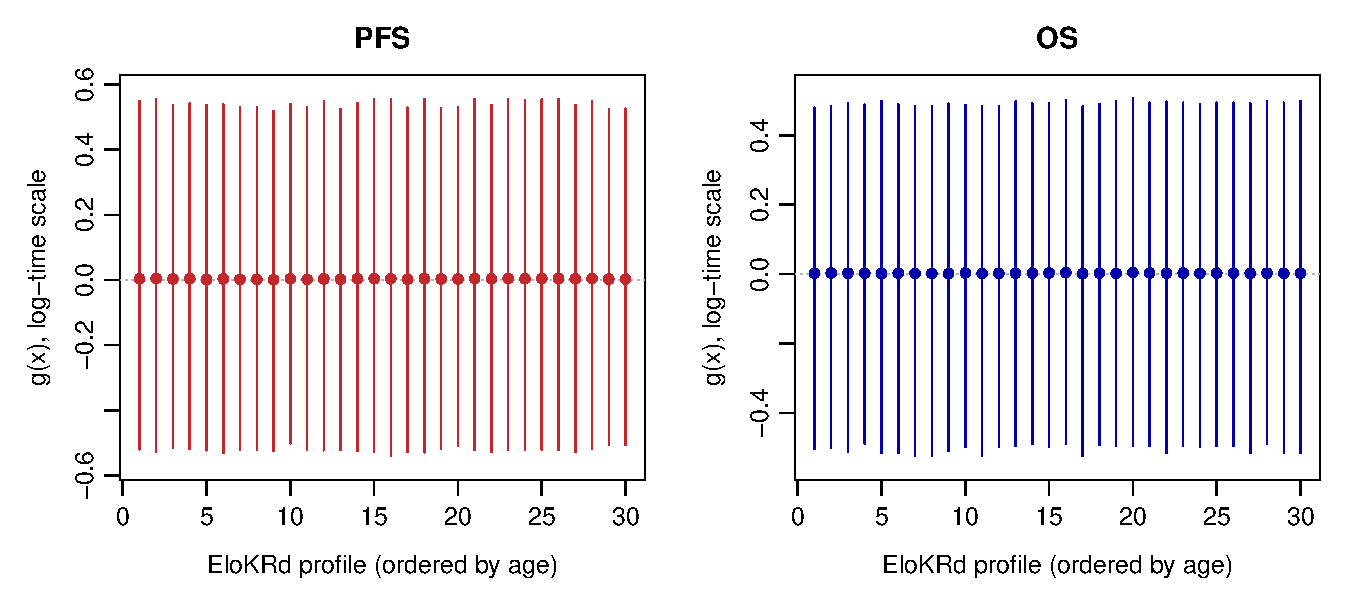
\includegraphics[width=\textwidth]{figures/fig_g_profiles.pdf}
\caption{Posterior mean and 95\% interval of the discrepancy $g(x)$ on the log-time scale at the 30 EloKRd profiles, ordered by age, at $N_{\rm target}=30$ for PFS (red) and OS (blue). In single-arm mode $g$ is a prior draw, so the intervals are centred at zero with SD $0.26$ everywhere; \DIFaddbeginFL \DIFaddFL{discrepancy uncertainty is therefore }\DIFaddendFL the \DIFdelbeginFL \DIFdelFL{figure documents that no }\DIFdelendFL \DIFaddbeginFL \DIFaddFL{same at every }\DIFaddendFL profile\DIFaddbeginFL \DIFaddFL{. Variation in external support }\DIFaddendFL is \DIFdelbeginFL \DIFdelFL{treated differently, which is why }\DIFdelendFL \DIFaddbeginFL \DIFaddFL{summarized by }\DIFaddendFL the \DIFdelbeginFL \DIFdelFL{covariate-resolved display for a single-arm analysis is the }\DIFdelendFL local ESS map \DIFdelbeginFL \DIFdelFL{of }\DIFdelendFL \DIFaddbeginFL \DIFaddFL{in }\DIFaddendFL Figure~\ref{fig:essmap}.}
\label{fig:gprofiles}
\end{figure}

\begin{figure}[htbp]
\centering
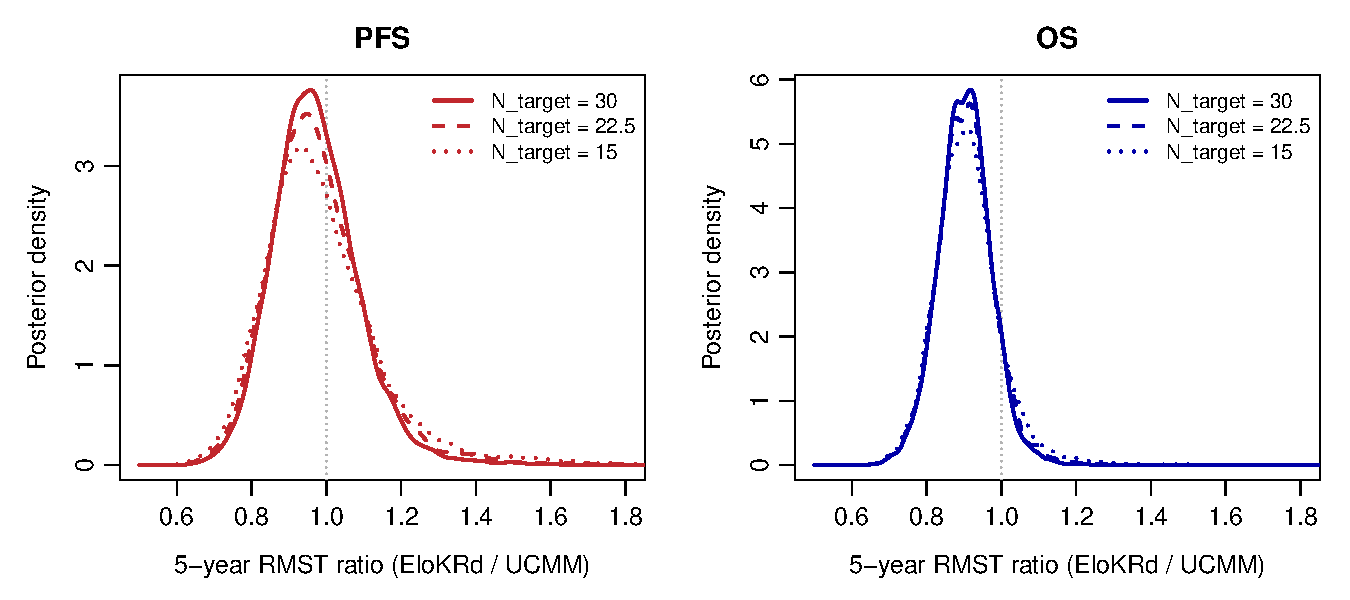
\includegraphics[width=\textwidth]{figures/fig_rmst_posterior.pdf}
\caption{Posterior density of the standardized 5-year RMST ratio for PFS and OS under LRC-BART at $N_{\rm target}=30$, $22.5$ and $15$ (harmonized coding, $H_f=10$, $w=1$).}
\label{fig:rmstpost}
\end{figure}

\subsection*{G.6 The prior cost of a regional shift in a shared-leaf design}

Section~\ref{sec:model} states that the decomposition into a pooled surface $f$ and a discrepancy ensemble $g$ is what lets a regional shift be detected, and we give the calculation here because the alternative, one ensemble with two means per leaf coupled through a common variance, looks equally natural. Suppose the RWD surface is shifted by $\delta$ on a region. In the shared-leaf design with $H$ trees and a commensurate scale $\tau^2$, the cheapest fit spreads $\delta/H$ across every tree under the spike, at prior cost $\delta^2/(2H\tau^2)$; routing the shift through $m$ slab leaves of variance $\lambda^2$ instead costs $m\,c+\delta^2/(2m\lambda^2)$ with $c$ the log prior odds plus the log ratio of the two scales, and the slab route is cheaper only if $\delta>2H\tau^2\sqrt{2c}/\lambda$. At $H=50$ and the scales of our simulation study this threshold is between $17$ and $86$ on an outcome with range $10$, so no shift of clinical size flips an indicator and the borrowing map stays flat. In the decomposition \eqref{eq:model} the shift lands in one or two leaves of one $g$ tree after a single split on the region boundary, which the tree prior allows at ordinary cost, and the slab wins as soon as $\tfrac{\delta^2}2\{(H_g\tau_0^2)^{-1}-\tau_1^{-2}\}$ exceeds the slab's prior cost $\log\tfrac w{1-w}+\log\tfrac{\tau_1}{\tau_0}$. The design keeps $H_g$ small on purpose: with few trees and a small $\tau_0$, the spike cannot hide a shift by spreading it. Letting $f$ absorb part of the shift misfits both sources and pays in the likelihood in proportion to $n_1+n_2$.

\subsection*{G.7 The single-arm simulation in detail}

\DIFdelbegin \DIFdel{Section~\ref{sec:sim_single} summarizes }\DIFdelend \DIFaddbegin \DIFadd{We provide further details of }\DIFaddend the single-arm study \DIFdelbegin \DIFdel{; this section gives the full account}\DIFdelend \DIFaddbegin \DIFadd{in Section~\ref{sec:sim_single}}\DIFaddend . The trial contributes $n_T$ treated subjects only, $200$ for Gaussian outcomes and $30$ or $200$ for survival outcomes, the $300$ RWD controls are the sole control source, and the estimands are standardized to the trial profiles. The comparators reduce to the complete-pooling models, the hierarchical models, BART-CP, and LRC-BART in the single-arm mode of Section~\ref{sec:singlearm} with $w=1$, at the absolute target $100$, at $0.9$ of the ceiling, and with the spike scale at the grid minimum, which is near-complete pooling of the leaf means; $w=0.9$ is the slab sensitivity. Sc3 is not identifiable without an internal control and is omitted. Table~\ref{tab:single} and Web Table~S6 report the results.

Under Sc1\DIFdelbegin \DIFdel{the tree models behave as expected: }\DIFdelend \DIFaddbegin \DIFadd{, }\DIFaddend BART-CP, the pooled LRC-BART and the target-$100$ LRC-BART have Gaussian RMSE $0.16$ with coverage $0.94$ to $1.00$, and at $n_T=30$ the survival RMST ratio has RMSE $0.16$ to $0.19$ with coverage $0.92$ to $0.97$. 
\DIFaddbegin 

\DIFaddend Under Sc2\DIFdelbegin \DIFdel{no method does well}\DIFdelend \DIFaddbegin \DIFadd{, all methods have substantial bias}\DIFaddend . With the source assignment of Sc2 and no RCT controls, the RWD is the only information about the control surface at trial profiles that lie where \DIFdelbegin \DIFdel{the RWD is thin}\DIFdelend \DIFaddbegin \DIFadd{RWD support is limited}\DIFaddend , and every method is far more biased than in the two-arm study: on the Gaussian ATE, LM-CP has bias $1.68$, BART-CP $0.41$ with coverage $0.75$, and LRC-BART $0.42$, and the survival median ratio at $n_T=30$ has biases of $0.8$ to $1.3$ for the tree models. Single-arm borrowing under measured confounding is a harder problem than the two-arm study, because nothing in the data can reveal a discrepancy at profiles the RWD does not cover; the rows reported for this scenario in the earlier version came from a different mechanism (Web Appendix~G.2). 
\DIFdelbegin \DIFdel{Two further points concern }\DIFdelend \DIFaddbegin 

\DIFadd{For }\DIFaddend LRC-BART\DIFdelbegin \DIFdel{. First, }\DIFdelend \DIFaddbegin \DIFadd{, uncertainty depends on whether the target is capped. }\DIFaddend LRC-BART ($100$) gives the same point estimate as the pooled model in every design, within $0.005$, and the same posterior wherever the target is capped: the single-arm ceiling is $27$ to $34$ in Sc2 and $75$ at $n_T=30$ in Sc1, so the absolute target is capped there, and where it is not, about $160$ in Sc1 at $n_T=200$, the prior draw of $g$ widens the posterior without moving it (Web Table~S6); the fractional rung at $0.9$ of the ceiling gives the same point estimates with wider intervals and coverage $0.82$ to $0.99$, \DIFdelbegin \DIFdel{which is what a single-arm calibration can offer. 
Second, the }\DIFdelend \DIFaddbegin \DIFadd{reflecting the role of calibration in controlling prior uncertainty. 
}

\DIFadd{The }\DIFaddend $w=0.9$ sensitivity has a posterior SD of $1.4$ on the Gaussian ATE and of $10$ to $34$ on the median ratio with power $0$ and coverage $1$, the point estimate unchanged, because with no RCT controls the slab draws add prior noise of variance $(1-w)H_g\tau_1^2$ to the counterfactual control and nothing else, which is why we report $w=1$ in single-arm mode. HierLM and HierAFT with the stated hyperprior and no RCT controls draw the control surface from the hierarchy, and their posterior SDs are $8$ on the Gaussian ATE and \DIFdelbegin \DIFdel{astronomically }\DIFdelend \DIFaddbegin \DIFadd{extremely }\DIFaddend large on the median ratio; \DIFdelbegin \DIFdel{we report }\DIFdelend \DIFaddbegin \DIFadd{these results make }\DIFaddend the stated model \DIFdelbegin \DIFdel{as unusable instead of tuning it }\DIFdelend \DIFaddbegin \DIFadd{unusable in this setting }\DIFaddend (Web Appendix~G.2).

\begin{center}
\scriptsize
\setlength{\tabcolsep}{3pt}
\renewcommand{\arraystretch}{0.8}
\begin{longtable}{llcccccccc}
\caption{Single-arm design, all methods, $R=500$. Columns as in Table~\ref{tab:single}; LRC-BART (100) and LRC-BART ($w=0.9$) use the absolute target 100, capped at the ceiling where infeasible, and LRC-BART (0.9, $w=0.9$) the fractional target with the slab.}\label{tab:single_full}\\
\toprule
& & \multicolumn{5}{c}{Treatment effect} & \multicolumn{2}{c}{Control} & \\
\cmidrule(lr){3-7}\cmidrule(lr){8-9}
Design & Method & Bias & SD & RMSE & Cov & Pow & Bias & RMSE & Prior ESS \\
\midrule
\endfirsthead
\multicolumn{10}{l}{\textit{Web Table S6, continued}}\\
\toprule
& & \multicolumn{5}{c}{Treatment effect} & \multicolumn{2}{c}{Control} & \\
\cmidrule(lr){3-7}\cmidrule(lr){8-9}
Design & Method & Bias & SD & RMSE & Cov & Pow & Bias & RMSE & Prior ESS \\
\midrule
\endhead
\midrule
\multicolumn{10}{r}{\textit{continued on the next page}}\\
\endfoot
\bottomrule
\endlastfoot
\multirow{8}{*}{\shortstack[l]{Gaussian, $n_T=200$\\ATE\\Sc1}} & LM-CP & 0.007 & 0.259 & 0.254 & 0.95 & 0.97 & $-$0.003 & 0.233 & --- \\
& HierLM & $-$0.014 & 8.239 & 0.497 & 1.00 & 0.00 & 0.018 & 0.487 & --- \\
& BART-CP & 0.010 & 0.163 & 0.162 & 0.94 & 1.00 & $-$0.003 & 0.127 & --- \\
& LRC-BART (pooled) & 0.007 & 0.165 & 0.162 & 0.94 & 1.00 & 0.001 & 0.127 & 172.3 \\
& LRC-BART (100) & 0.006 & 0.252 & 0.161 & 1.00 & 1.00 & 0.001 & 0.127 & 81.9 \\
& LRC-BART (0.9) & 0.007 & 0.202 & 0.163 & 0.98 & 1.00 & 0.000 & 0.128 & 115.8 \\
& LRC-BART ($w=0.9$) & 0.010 & 1.383 & 0.169 & 1.00 & 0.00 & $-$0.003 & 0.136 & 81.9 \\
& LRC-BART (0.9, $w=0.9$) & 0.006 & 1.372 & 0.169 & 1.00 & 0.00 & 0.001 & 0.133 & 116.4 \\
\midrule
\multirow{8}{*}{\shortstack[l]{Gaussian, $n_T=200$\\ATE\\Sc2}} & LM-CP & 1.682 & 0.417 & 1.734 & 0.01 & 1.00 & $-$1.676 & 1.726 & --- \\
& HierLM & 1.642 & 8.317 & 1.754 & 1.00 & 0.00 & $-$1.636 & 1.747 & --- \\
& BART-CP & 0.408 & 0.310 & 0.506 & 0.75 & 1.00 & $-$0.399 & 0.492 & --- \\
& LRC-BART (pooled) & 0.420 & 0.316 & 0.515 & 0.75 & 1.00 & $-$0.412 & 0.501 & 34.8 \\
& LRC-BART (100) & 0.421 & 0.316 & 0.515 & 0.76 & 1.00 & $-$0.413 & 0.501 & 34.7 \\
& LRC-BART (0.9) & 0.417 & 0.416 & 0.511 & 0.89 & 0.98 & $-$0.409 & 0.498 & 23.1 \\
& LRC-BART ($w=0.9$) & 0.416 & 1.329 & 0.511 & 1.00 & 0.00 & $-$0.408 & 0.498 & 34.8 \\
& LRC-BART (0.9, $w=0.9$) & 0.420 & 1.345 & 0.514 & 1.00 & 0.00 & $-$0.411 & 0.500 & 23.0 \\
\midrule
\multirow{8}{*}{\shortstack[l]{Survival, $n_T=30$\\median ratio\\Sc1}} & AFT-CP & 1.540 & 4.678 & 4.444 & 0.92 & 0.15 & $-$0.006 & 0.204 & --- \\
& HierAFT & $>\!10^{3}$ & $>\!10^{3}$ & $>\!10^{3}$ & 1.00 & 0.00 & $>\!10^{3}$ & $>\!10^{3}$ & --- \\
& BART-CP & $-$0.013 & 0.580 & 0.482 & 0.97 & 0.05 & $-$0.026 & 0.103 & --- \\
& LRC-BART (pooled) & 0.182 & 0.918 & 0.686 & 0.98 & 0.02 & $-$0.017 & 0.102 & 80.2 \\
& LRC-BART (100) & 0.180 & 0.917 & 0.686 & 0.98 & 0.03 & $-$0.017 & 0.099 & 79.0 \\
& LRC-BART (0.9) & 0.222 & 1.174 & 0.711 & 0.99 & 0.01 & $-$0.005 & 0.133 & 51.8 \\
& LRC-BART ($w=0.9$) & 1.423 & 11.199 & 1.959 & 1.00 & 0.00 & 0.318 & 0.433 & 79.3 \\
& LRC-BART (0.9, $w=0.9$) & 1.555 & 13.493 & 2.257 & 1.00 & 0.00 & 0.335 & 0.469 & 52.2 \\
\midrule
\multirow{8}{*}{\shortstack[l]{Survival, $n_T=30$\\median ratio\\Sc2}} & AFT-CP & 20.944 & 46.014 & 51.645 & 0.19 & 0.89 & $-$0.441 & 0.526 & --- \\
& HierAFT & $>\!10^{3}$ & $>\!10^{3}$ & $>\!10^{3}$ & 1.00 & 0.00 & $>\!10^{3}$ & $>\!10^{3}$ & --- \\
& BART-CP & 0.814 & 1.109 & 1.231 & 0.92 & 0.25 & $-$0.199 & 0.277 & --- \\
& LRC-BART (pooled) & 1.324 & 1.859 & 1.864 & 0.95 & 0.21 & $-$0.207 & 0.284 & 29.2 \\
& LRC-BART (100) & 1.329 & 1.865 & 1.875 & 0.95 & 0.20 & $-$0.208 & 0.284 & 29.1 \\
& LRC-BART (0.9) & 1.511 & 3.461 & 2.055 & 0.97 & 0.12 & $-$0.180 & 0.279 & 19.3 \\
& LRC-BART ($w=0.9$) & 4.243 & 28.669 & 5.305 & 1.00 & 0.00 & 0.179 & 0.537 & 28.9 \\
& LRC-BART (0.9, $w=0.9$) & 4.544 & 33.228 & 6.324 & 1.00 & 0.00 & 0.193 & 0.446 & 19.0 \\
\midrule
\multirow{8}{*}{\shortstack[l]{Survival, $n_T=30$\\RMST ratio\\Sc1}} & AFT-CP & 0.036 & 0.178 & 0.202 & 0.90 & 0.16 & 0.079 & 0.187 & --- \\
& HierAFT & $>\!10^{3}$ & $>\!10^{3}$ & $>\!10^{3}$ & 1.00 & 0.00 & 0.311 & 0.355 & --- \\
& BART-CP & $-$0.111 & 0.176 & 0.186 & 0.92 & 0.02 & $-$0.021 & 0.089 & --- \\
& LRC-BART (pooled) & $-$0.046 & 0.192 & 0.157 & 0.97 & 0.02 & 0.002 & 0.085 & 80.2 \\
& LRC-BART (100) & $-$0.046 & 0.192 & 0.157 & 0.97 & 0.02 & 0.002 & 0.084 & 79.0 \\
& LRC-BART (0.9) & $-$0.040 & 0.218 & 0.156 & 0.98 & 0.01 & 0.002 & 0.085 & 51.8 \\
& LRC-BART ($w=0.9$) & 0.080 & 0.998 & 0.200 & 1.00 & 0.00 & 0.020 & 0.089 & 79.3 \\
& LRC-BART (0.9, $w=0.9$) & 0.086 & 1.077 & 0.204 & 1.00 & 0.00 & 0.020 & 0.090 & 52.2 \\
\midrule
\multirow{8}{*}{\shortstack[l]{Survival, $n_T=30$\\RMST ratio\\Sc2}} & AFT-CP & 1.216 & 0.522 & 1.336 & 0.13 & 0.94 & $-$0.518 & 0.559 & --- \\
& HierAFT & $>\!10^{3}$ & $>\!10^{3}$ & $>\!10^{3}$ & 1.00 & 0.00 & 0.017 & 0.201 & --- \\
& BART-CP & 0.149 & 0.271 & 0.286 & 0.95 & 0.14 & $-$0.219 & 0.260 & --- \\
& LRC-BART (pooled) & 0.234 & 0.297 & 0.339 & 0.94 & 0.19 & $-$0.210 & 0.251 & 29.2 \\
& LRC-BART (100) & 0.235 & 0.297 & 0.340 & 0.94 & 0.19 & $-$0.211 & 0.251 & 29.1 \\
& LRC-BART (0.9) & 0.256 & 0.452 & 0.358 & 0.97 & 0.13 & $-$0.207 & 0.248 & 19.3 \\
& LRC-BART ($w=0.9$) & 0.527 & 2.689 & 0.643 & 1.00 & 0.00 & $-$0.185 & 0.228 & 28.9 \\
& LRC-BART (0.9, $w=0.9$) & 0.560 & 3.085 & 0.731 & 1.00 & 0.00 & $-$0.184 & 0.228 & 19.0 \\
\midrule
\multirow{8}{*}{\shortstack[l]{Survival, $n_T=200$\\median ratio\\Sc1}} & AFT-CP & 0.168 & 0.470 & 0.480 & 0.95 & 0.23 & 0.002 & 0.098 & --- \\
& HierAFT & $>\!10^{3}$ & $>\!10^{3}$ & $>\!10^{3}$ & 1.00 & 0.00 & $>\!10^{3}$ & $>\!10^{3}$ & --- \\
& BART-CP & 0.108 & 0.273 & 0.286 & 0.95 & 0.57 & $-$0.026 & 0.058 & --- \\
& LRC-BART (pooled) & 0.076 & 0.272 & 0.262 & 0.97 & 0.49 & $-$0.018 & 0.055 & 169.5 \\
& LRC-BART (100) & 0.108 & 0.565 & 0.284 & 1.00 & 0.17 & $-$0.008 & 0.055 & 81.7 \\
& LRC-BART (0.9) & 0.087 & 0.350 & 0.268 & 0.99 & 0.34 & $-$0.014 & 0.055 & 114.0 \\
& LRC-BART ($w=0.9$) & 1.492 & 15.408 & 4.227 & 1.00 & 0.00 & 0.318 & 0.402 & 81.8 \\
& LRC-BART (0.9, $w=0.9$) & 1.302 & 10.341 & 1.607 & 1.00 & 0.00 & 0.312 & 0.428 & 113.7 \\
\midrule
\multirow{8}{*}{\shortstack[l]{Survival, $n_T=200$\\median ratio\\Sc2}} & AFT-CP & 9.478 & 5.162 & 10.850 & 0.01 & 1.00 & $-$0.407 & 0.419 & --- \\
& HierAFT & $>\!10^{3}$ & $>\!10^{3}$ & $>\!10^{3}$ & 1.00 & 0.00 & $>\!10^{3}$ & $>\!10^{3}$ & --- \\
& BART-CP & 1.136 & 0.778 & 1.359 & 0.60 & 0.82 & $-$0.189 & 0.214 & --- \\
& LRC-BART (pooled) & 1.195 & 0.851 & 1.409 & 0.64 & 0.82 & $-$0.196 & 0.219 & 35.9 \\
& LRC-BART (100) & 1.193 & 0.856 & 1.410 & 0.65 & 0.81 & $-$0.196 & 0.219 & 35.9 \\
& LRC-BART (0.9) & 1.336 & 2.306 & 1.562 & 0.82 & 0.57 & $-$0.181 & 0.207 & 23.9 \\
& LRC-BART ($w=0.9$) & 3.935 & 26.373 & 4.611 & 1.00 & 0.00 & 0.142 & 0.396 & 36.2 \\
& LRC-BART (0.9, $w=0.9$) & 4.380 & 34.059 & 7.322 & 1.00 & 0.00 & 0.158 & 0.379 & 23.8 \\
\midrule
\multirow{8}{*}{\shortstack[l]{Survival, $n_T=200$\\RMST ratio\\Sc1}} & AFT-CP & $-$0.023 & 0.101 & 0.098 & 0.94 & 0.15 & 0.074 & 0.114 & --- \\
& HierAFT & $>\!10^{3}$ & $>\!10^{3}$ & $>\!10^{3}$ & 1.00 & 0.00 & 0.305 & 0.317 & --- \\
& BART-CP & $-$0.001 & 0.084 & 0.082 & 0.97 & 0.32 & $-$0.021 & 0.061 & --- \\
& LRC-BART (pooled) & $-$0.024 & 0.078 & 0.076 & 0.95 & 0.25 & 0.001 & 0.054 & 169.5 \\
& LRC-BART (100) & $-$0.020 & 0.121 & 0.076 & 0.99 & 0.09 & 0.003 & 0.054 & 81.7 \\
& LRC-BART (0.9) & $-$0.022 & 0.094 & 0.076 & 0.99 & 0.17 & 0.002 & 0.054 & 114.0 \\
& LRC-BART ($w=0.9$) & 0.109 & 1.179 & 0.275 & 1.00 & 0.00 & 0.021 & 0.057 & 81.8 \\
& LRC-BART (0.9, $w=0.9$) & 0.097 & 0.860 & 0.138 & 1.00 & 0.00 & 0.019 & 0.057 & 113.7 \\
\midrule
\multirow{8}{*}{\shortstack[l]{Survival, $n_T=200$\\RMST ratio\\Sc2}} & AFT-CP & 1.164 & 0.428 & 1.244 & 0.01 & 1.00 & $-$0.535 & 0.550 & --- \\
& HierAFT & $>\!10^{3}$ & $>\!10^{3}$ & $>\!10^{3}$ & 1.00 & 0.00 & 0.001 & 0.101 & --- \\
& BART-CP & 0.305 & 0.206 & 0.361 & 0.61 & 0.77 & $-$0.233 & 0.261 & --- \\
& LRC-BART (pooled) & 0.284 & 0.206 & 0.336 & 0.70 & 0.74 & $-$0.224 & 0.250 & 35.9 \\
& LRC-BART (100) & 0.284 & 0.207 & 0.336 & 0.69 & 0.73 & $-$0.224 & 0.250 & 35.9 \\
& LRC-BART (0.9) & 0.301 & 0.350 & 0.353 & 0.85 & 0.50 & $-$0.222 & 0.248 & 23.9 \\
& LRC-BART ($w=0.9$) & 0.562 & 2.419 & 0.633 & 1.00 & 0.00 & $-$0.200 & 0.228 & 36.2 \\
& LRC-BART (0.9, $w=0.9$) & 0.585 & 2.496 & 0.662 & 1.00 & 0.00 & $-$0.198 & 0.226 & 23.8 \\
\end{longtable}
\end{center}


\end{document}
